% \DeclareDocumentMetadata {lang=en-US}

% xmp metadata for pdf
% Originally used \usepackage[a-2a]{pdfx}
% \usepackage{hyperxmp} replaced it
% \RequirePackage{pdfmanagement-testphase} replaced it
% \PassOptionsToPackage{enable-debug,check-declarations}{expl3} broke with version 0.9 of tagpdf
% \ExplSyntaxOn no need for these 3 lines because metadata can handle it
% \pdfmanagement_add:nnn{Catalog}{Lang}{(enUS)} enUS is wrong, should be en-US
% \ExplSyntaxOff

\documentclass[11pt,
  english,
  letterpaper,
]{article}
\usepackage{sa4ss}
\usepackage{amsmath,amssymb,array}
\usepackage{booktabs}

% From tagged-template.latex
\usepackage{lmodern}
\usepackage{ifxetex,ifluatex}
\ifnum 0\ifxetex 1\fi\ifluatex 1\fi=0 % if pdftex
  \usepackage[T1]{fontenc}
  \usepackage[utf8]{inputenc}
  \usepackage{textcomp} % provide euro and other symbols
\else % if luatex or xetex
  \usepackage{unicode-math}
  \defaultfontfeatures{Scale=MatchLowercase}
  \defaultfontfeatures[\rmfamily]{Ligatures=TeX,Scale=1}
\fi

% Use upquote if available, for straight quotes in verbatim environments
\IfFileExists{upquote.sty}{\usepackage{upquote}}{}
\IfFileExists{microtype.sty}{% use microtype if available
  \usepackage[]{microtype}
  \UseMicrotypeSet[protrusion]{basicmath} % disable protrusion for tt fonts
}{}
\makeatletter
\@ifundefined{KOMAClassName}{% if non-KOMA class
  \IfFileExists{parskip.sty}{%
    \usepackage{parskip}
  }{% else
    \setlength{\parindent}{0pt}
    \setlength{\parskip}{6pt plus 2pt minus 1pt}}
}{% if KOMA class
  \KOMAoptions{parskip=half}}
\makeatother
\usepackage{xcolor}
\IfFileExists{xurl.sty}{\usepackage{xurl}}{} % add URL line breaks if available
\hypersetup{
  pdftitle={Status of Shortspine Thornyhead (Sebastolobus alascanus) along the US West coast in 2023},
  pdflang={en},
  hidelinks,
  pdfcreator={LaTeX via pandoc}}
\urlstyle{same} % disable monospaced font for URLs
\usepackage{longtable}
% Correct order of tables after \paragraph or \subparagraph
\usepackage{etoolbox}
\makeatletter
\patchcmd\longtable{\par}{\if@noskipsec\mbox{}\fi\par}{}{}
\makeatother
% Allow footnotes in longtable head/foot
\IfFileExists{footnotehyper.sty}{\usepackage{footnotehyper}}{\usepackage{footnote}}
\makesavenoteenv{longtable}
\usepackage{graphicx}
\makeatletter
\def\maxwidth{\ifdim\Gin@nat@width>\linewidth\linewidth\else\Gin@nat@width\fi}
\def\maxheight{\ifdim\Gin@nat@height>\textheight\textheight\else\Gin@nat@height\fi}
\makeatother
% Scale images if necessary, so that they will not overflow the page
% margins by default, and it is still possible to overwrite the defaults
% using explicit options in \includegraphics[width, height, ...]{}
\setkeys{Gin}{width=\maxwidth,height=\maxheight,keepaspectratio}
% Set default figure placement to htbp
\makeatletter
\def\fps@figure{htbp}
\makeatother
\setlength{\emergencystretch}{3em} % prevent overfull lines
\providecommand{\tightlist}{%
  \setlength{\itemsep}{0pt}\setlength{\parskip}{0pt}}
\setcounter{secnumdepth}{5}
\ifxetex
  % Load polyglossia as late as possible: uses bidi with RTL langages (e.g. Hebrew, Arabic)
  \usepackage{polyglossia}
  \setmainlanguage[]{english}
\else
  \usepackage[shorthands=off,main=english]{babel}
\fi

%Define cslreferences environment, required by pandoc 2.8
%https://github.com/rstudio/rmarkdown/issues/1649
\newlength{\csllabelwidth}
\setlength{\csllabelwidth}{3em}
\newlength{\cslhangindent}
\setlength{\cslhangindent}{1.5em}
% for Pandoc 2.8 to 2.10.1
\newenvironment{cslreferences}%
  {}%
  {\par}
% For Pandoc 2.11+
\newenvironment{CSLReferences}[2] % #1 hanging-ident, #2 entry spacing
 {% don't indent paragraphs
  \setlength{\parindent}{0pt}
  % turn on hanging indent if param 1 is 1
  \ifodd #1 \everypar{\setlength{\hangindent}{\cslhangindent}}\ignorespaces\fi
  % set entry spacing
  \ifnum #2 > 0
  \setlength{\parskip}{#2\baselineskip}
  \fi
 }%
 {}
\usepackage{calc}  % for \widthof, \maxof in minipage
\newcommand{\CSLBlock}[1]{#1\hfill\break}
\newcommand{\CSLLeftMargin}[1]{\parbox[t]{\csllabelwidth}{#1}}
\newcommand{\CSLRightInline}[1]{\parbox[t]{\linewidth - \csllabelwidth}{#1}\break}
\newcommand{\CSLIndent}[1]{\hspace{\cslhangindent}#1}


\providecommand{\tightlist}{%
  \setlength{\itemsep}{0pt}\setlength{\parskip}{0pt}}


\date{}
\newcommand{\trTitle}{Status of Shortspine Thornyhead (\emph{Sebastolobus alascanus}) along the US West coast in 2023}
\newcommand{\trYear}{2023}
\newcommand{\trMonth}{May}
\newcommand{\trAuthsLong}{truetruetruetruetruetruetruetruetrue}
\newcommand{\trAuthsBack}{Zahner. J.A, M.A.~Heller-Shipley, S. Beyer, A.L. Hayes, P-Y. Hernvann, A.N. Odell, H. Oleynik, J.Y. Sullivan, M. Veron}
\newcommand{\trCitation}{
\begin{hangparas}{1em}{1}
\trAuthsBack{}. \trYear{}. \trTitle{}. \glsentrylong{pfmc}, Portland, Oregon. \pageref{LastPage}{}\,p.
\end{hangparas}}

\begin{document}

%%%%% Frontmatter %%%%%

% Footnote symbols in front matter
\renewcommand*{\thefootnote}{\fnsymbol{footnote}}

\small
\thispagestyle{empty}
\pagenumbering{roman}
\noindent
\begin{center}
\title{Status of Shortspine Thornyhead (\emph{Sebastolobus alascanus}) along the US West coast in 2023}
% \textnormal{\MakeTextUppercase{\trTitle{}}}
\vspace{1.5cm}
{\Large\textbf\newline{Status of Shortspine Thornyhead (\emph{Sebastolobus alascanus}) along the US West coast in 2023}}
\vfill
by\\
Joshua Zahner\textsuperscript{1}\\
Madison Heller-Shipley\textsuperscript{1}\\
Sabrina Beyer\textsuperscript{1}\\
Adam Hayes\textsuperscript{1}\\
Pierre-Yves Hernvann\textsuperscript{2}\\
Andrea Odell\textsuperscript{3}\\
Haley Oleynik\textsuperscript{4}\\
Jane Y. Sullivan\textsuperscript{5}\\
Matthieu Veron\textsuperscript{6}\vfill
\textsuperscript{1}School of Aquatic and Fishery Sciences, University of Washington, 1122 NE Boat Street, Seattle, Washington 98195\\
\textsuperscript{2}Northwest Fisheries Science Center, U.S. Department of Commerce, National Oceanic and Atmospheric Administration, National Marine Fisheries Service, 2725 Montlake Boulevard East, Seattle, Washington 98112\\
\textsuperscript{3}University of California Davis, One Shields Avenue, Davis, California 95616\\
\textsuperscript{4}Institute for the Oceans and Fisheries, University of British Columbia, 2202 Main Mall, Vancouver, British Columbia Canada V6T 1Z4\\
\textsuperscript{5}Alaska Fisheries Science Center, U.S. Department of Commerce, National Oceanic and Atmospheric Administration, National Marine Fisheries Service, 17109 Point Lena Loop Road, Juneau, Alaska 99801\\
\textsuperscript{6}Alaska Fisheries Science Center, U.S. Department of Commerce, National Oceanic and Atmospheric Administration, National Marine Fisheries Service, 7600 Sand Point Way N.E., Seattle, Washington 98115\vfill
\trMonth{} \trYear{}
\end{center}
\clearpage

% Fourth page: Colophon
\thispagestyle{empty}
\vspace*{\fill}
\begin{center}
\copyright{} \glsentrylong{pfmc}, \trYear{}\\
\end{center}
\par
\bigskip
\noindent
Correct citation for this publication:
\bigskip
\par
\trCitation{}
\clearpage

% Add TOC to pdf bookmarks (clickable pdf)
\pdfbookmark[1]{\contentsname}{toc}

% Table of contents page, lists of figures and tables
\tableofcontents\clearpage
\label{TRlastRoman}
\clearpage

% Table of contents
\newpage
\thispagestyle{empty} % to remove page number

% Settings for the main document
\pagenumbering{arabic}  % Regular page numbers
\pagestyle{plain}  % No page number on first page of main document, use 'empty'
\renewcommand*{\thefootnote}{\arabic{footnote}}  % Back to numeric footnotes
\setcounter{footnote}{0}  % And start at 1
\renewcommand{\headrulewidth}{0.5pt}
\renewcommand{\footrulewidth}{0.5pt}
%\pagestyle{fancy}\fancyhead[c]{Draft: Do not cite or circulate}

\newcommand{\lt}{\ensuremath <}
\newcommand{\gt}{\ensuremath >}

\pagebreak
\pagenumbering{roman}
\setcounter{page}{1}

\renewcommand{\thetable}{\roman{table}}
\renewcommand{\thefigure}{\roman{figure}}

\setlength\parskip{0.5em plus 0.1em minus 0.2em}

\hypertarget{executive-summary}{%
\section*{Executive summary}\label{executive-summary}}
\addcontentsline{toc}{section}{Executive summary}

\hypertarget{stock}{%
\subsection*{Stock}\label{stock}}
\addcontentsline{toc}{subsection}{Stock}

This assessment applies to Shortspine thornyhead (Sebastolobus alascanus) off of the west coast of the United States from the U.S.-Canada border to the U.S.-Mexico border using data through 2023. Shortspine thornyheads are modeled in this assessment as a single stock. They have been reported as deep as 1,524 m, and this assessment applies to their full depth range although survey and fishery data are only available down to 1,280 m.

\hypertarget{catches}{%
\subsection*{Catches}\label{catches}}
\addcontentsline{toc}{subsection}{Catches}

Landings of shortspine are estimated to have risen to a peak of 4,815 mt in 1989, followed by a sharp decline during a period of trip limits and other management measures imposed in the 1990s. Since the institution of separate trip limits for shortspine and longspine thornyheads, the fishery had more moderate removals of between 1,000 and 2,000 mt per year from 1995 through 1998. Landings fell below 1,000 mt per year from 1999 through 2006, then rose to 1,531 in 2009 and have declined since that time. Recreational fishery landings of thornyheads were negligible, so only commercial landings were included in the model.

Commercial landings are dominantly bottom trawl caught, and non-trawl landings include all other gear types, the majority of which is longline. For this assessment, trawl landings were divided into North (the waters off Washington and Oregon) and South (the waters off California) fleets, and non-trawl landings represent one, coastwide fleet. Discard rates (landings divided by total catch) for shortspine have been estimated as high as 43\% per year, but are more frequently below 20\%. Discard rates in the trawl fleets, available from the West Coast Groundfish Observer Program (WCGOP), declined from 2003--2011 and have since increased from 2012-present, when the catch shares system began.

\begingroup\fontsize{10}{12}\selectfont
\begingroup\fontsize{10}{12}\selectfont

\begin{longtable}[t]{c>{\centering\arraybackslash}p{1.83cm}>{\centering\arraybackslash}p{1.83cm}>{\centering\arraybackslash}p{1.83cm}>{\centering\arraybackslash}p{1.83cm}>{\centering\arraybackslash}p{1.83cm}}
\caption{\label{tab:catches}Recent landings by fleet, total landings summed across fleets, and the total mortality including discards.}\\
\toprule
Year & North Trawl & South Trawl & Non-Trawl & Total Landings & Total Dead\\
\midrule
\endfirsthead
\caption[]{\label{tab:catches}Recent landings by fleet, total landings summed across fleets, and the total mortality including discards. \textit{(continued)}}\\
\toprule
Year & North Trawl & South Trawl & Non-Trawl & Total Landings & Total Dead\\
\midrule
\endhead

\endfoot
\bottomrule
\endlastfoot
2013 & 547.98 & 294.83 & 166.40 & 1,009.21 & 1,085.62\\
2014 & 433.12 & 254.05 & 147.81 & 834.98 & 900.66\\
2015 & 503.14 & 244.29 & 131.30 & 878.73 & 945.40\\
2016 & 577.19 & 185.73 & 168.94 & 931.86 & 1,012.75\\
2017 & 606.86 & 158.30 & 223.82 & 988.97 & 1,085.60\\
2018 & 525.04 & 105.07 & 184.48 & 814.60 & 895.39\\
2019 & 402.95 & 127.94 & 143.48 & 674.37 & 736.82\\
2020 & 248.47 & 87.99 & 85.17 & 421.64 & 458.87\\
2021 & 226.00 & 73.39 & 78.74 & 378.13 & 411.62\\
2022 & 261.16 & 97.61 & 66.22 & 424.98 & 456.65\\*
\end{longtable}
\endgroup{}
\endgroup{}

\begin{figure}
\centering
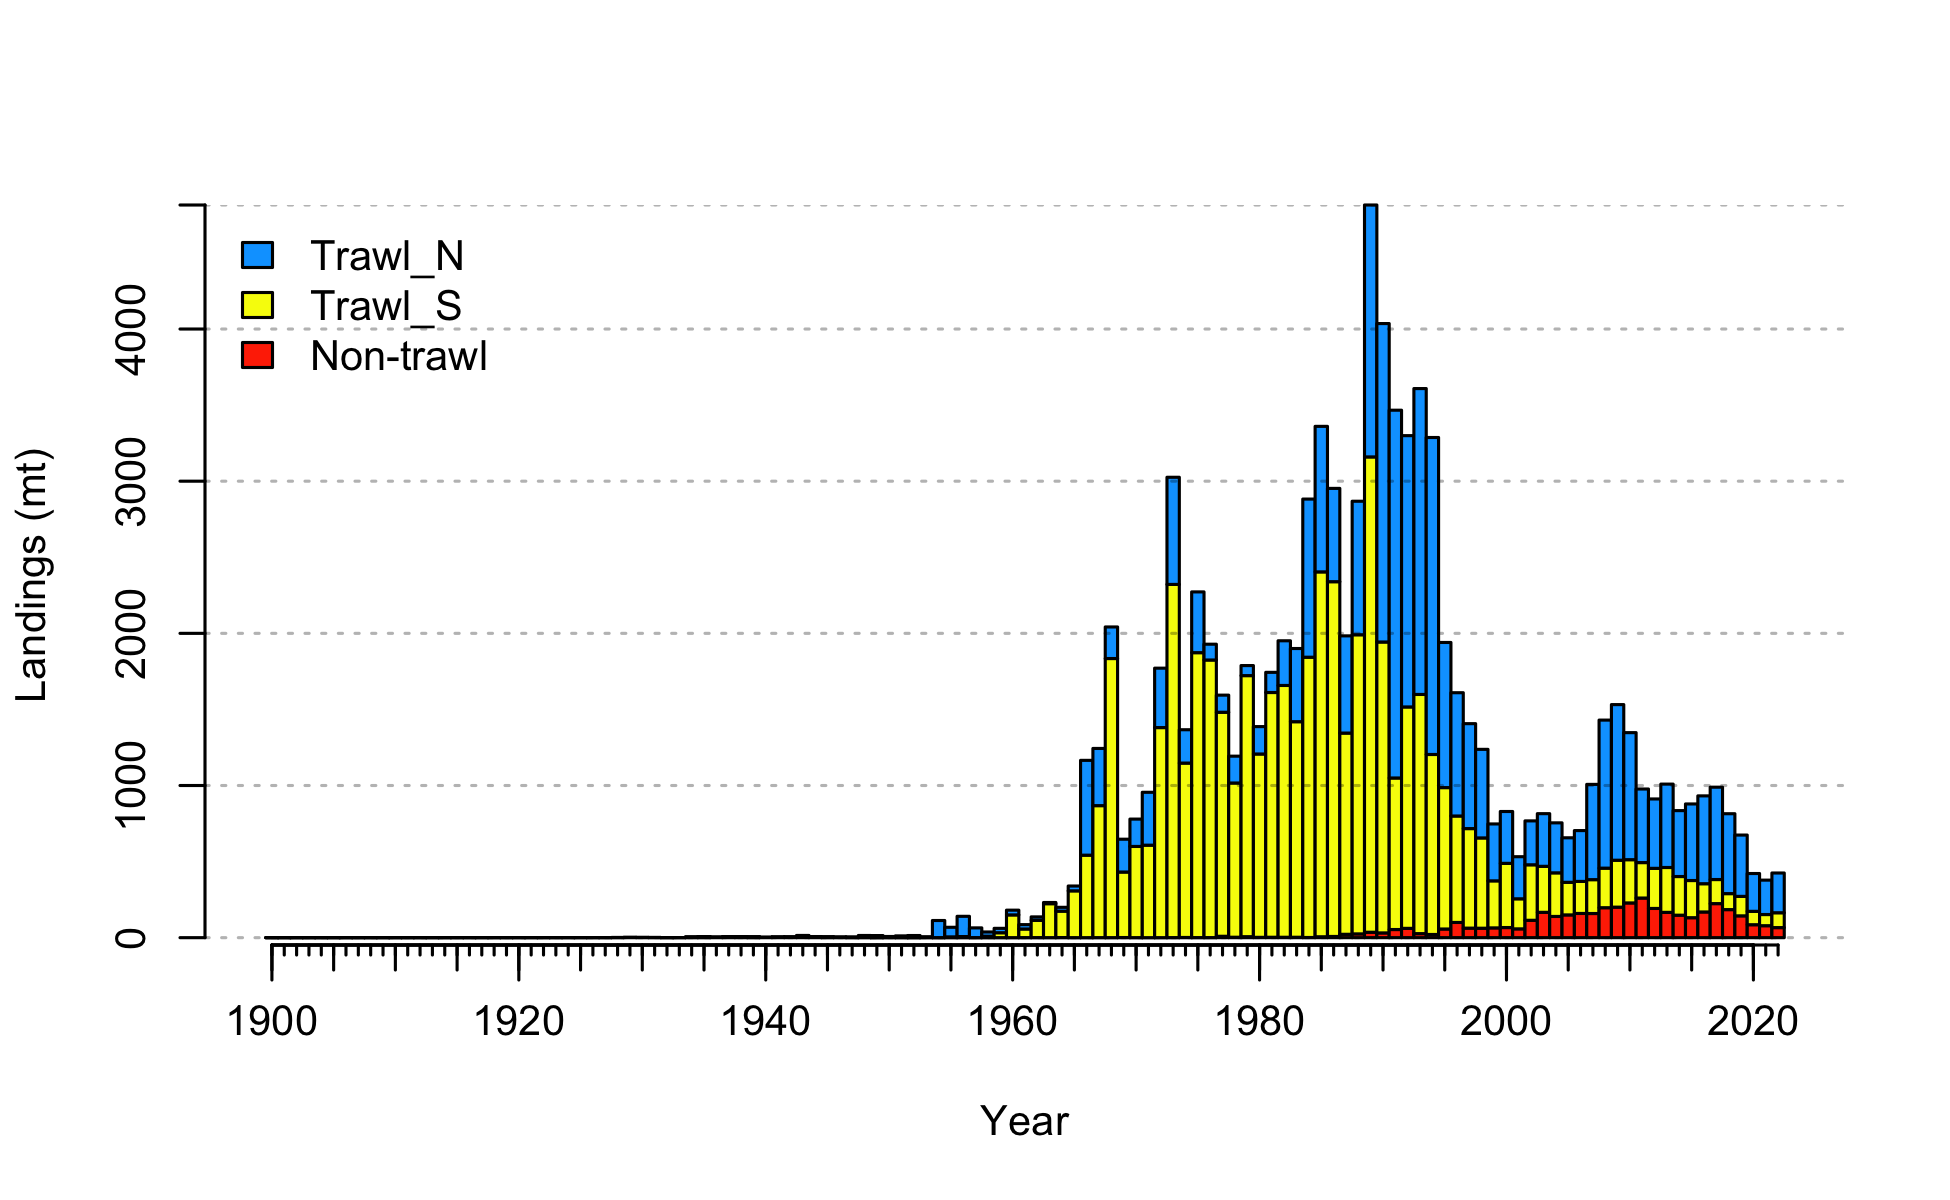
\includegraphics[width=1\textwidth,height=1\textheight]{/Users/jzahner/Desktop/Projects/shortspine_thornyhead_2023/doc/FinalFigs/Base/catch2 landings stacked.png}
\caption{Estimated landing history for shortspine thornyhead.\label{fig:catch_hist}}
\end{figure}

\hypertarget{data-and-assessment}{%
\subsection*{Data and assessment}\label{data-and-assessment}}
\addcontentsline{toc}{subsection}{Data and assessment}

The most recent assessment for shortspine thornyhead was conducted in 2012 (Taylor and Stephens 2013). Stock status was determined to be above the target biomass and catches did not attain the full management limits so reassessment of thornyheads has not been a higher priority. This assessment used Stock Synthesis (Methot and Wetzel 2013) Version 3.30.21, used in many other recent west coast assessments.

Data were divided into three fishery fleets: North trawl (the waters off Washington and Oregon), South trawl (the waters off California), and coastwide non-trawl, and three survey fleets: the Alaska Fishery Science Center (AFSC) Triennial Shelf Survey from 1980-2003, which was divided into early (pre-1995) and late period (post-1995) to account for a change in depth-sampling, and the West Coast Groundfish Bottom Trawl Survey (WCGBTS), 2004-2022.

Most data used in the 2012 assessment were newly pulled and processed for this assessment, including length compositions from all fishing and survey fleets, indices of abundance derived from new geostatistical analyses, discard rates from both a 1980s observer study (Pikitch et al., 1988) and the current WCGOP, historical catch data from Washington, Oregon, and California, and all reported catches from 1981-2022. The only data taken from the previous assessment without reanalysis were discard rates from the Enhanced Data Collection Project (EDCP) study in the 1990s.

New maturity analyses of samples collected in the WCGBTS in 2011, 2013, 2014, 2016 and 2018 were available for this assessment (M. Head, pers. comm.). The larger number and better spatial coverage of these samples allowed the use of statistical modeling to better understand the spatial variation in the proportion of female spawning. This assessment also assumes a new fecundity relationship, in which fecundity increases with body size. New growth curves were estimated, using data from Butler (1995), which were similar to the curves assumed in the 2005 and 2013 assessments. In the previous assessment, a Beverton-Holt stock recruitment relationship was assumed and steepness was fixed at 0.60. This assessment fixed steepness at 0.72, as recommended by Thorson et al. (2019). Natural mortality was also slightly updated from the 2013 assessment to be fixed at 0.04.

This assessment estimated 180 parameters. The log of the unfished equilibrium recruitment, log(R0), controls the scale of the population and annual deviations around the stock-recruit curve (135 parameters) allow for more uncertainty in the population trajectory. In addition, 43 selectivity and retention parameters for the three fishery fleets and three surveys allowed for estimation of annual length compositions and discards rates. Two catchability parameters were analytically computed from the data, and one additional parameter, representing additional variability in the early Triennial survey, was directly estimated by the model.

\hypertarget{stock-biomass-and-dynamics}{%
\subsection*{Stock biomass and dynamics}\label{stock-biomass-and-dynamics}}
\addcontentsline{toc}{subsection}{Stock biomass and dynamics}

Unfished equilibrium spawning output (B0) is estimated to be 20.332 trillion eggs, with a 95\% confidence interval of 16.338-24.327 trillion eggs. The B0 estimate here is not comparable to previous assessment as the integration of new fecundity and maturity assumptions have changed the output units from traditional biomass to spawned eggs. Spawning biomass is estimated to have remained stable until the early-1970s before beginning to decline near linearly through the present day. The estimated spawning output in 2023 is 8.372 trillion eggs, which represents a stock status or ``depletion'' (represented as spawning biomass in 2023, B2023, divided by B0) of 41.4\% (Figure XX). The depletion in 2013 was estimated to be 43.6\%, a large decrease from what was estimated in 2013 (\textasciitilde75\%).

\begingroup\fontsize{10}{12}\selectfont
\begingroup\fontsize{10}{12}\selectfont

\begin{longtable}[t]{c>{\centering\arraybackslash}p{2.2cm}>{\centering\arraybackslash}p{2.2cm}>{\centering\arraybackslash}p{2.2cm}>{\centering\arraybackslash}p{2.2cm}}
\caption{\label{tab:ssb}Spawning output (millions of eggs) and fraction unfished with associated 95\% confidence intervals (CI) from the base model.}\\
\toprule
Year & Spawning Output & Spawning Output 95\% CI & Fraction Unfished & Fraction Unfished 95\% CI\\
\midrule
\endfirsthead
\caption[]{\label{tab:ssb}Spawning output (millions of eggs) and fraction unfished with associated 95\% confidence intervals (CI) from the base model. \textit{(continued)}}\\
\toprule
Year & Spawning Output & Spawning Output 95\% CI & Fraction Unfished & Fraction Unfished 95\% CI\\
\midrule
\endhead

\endfoot
\bottomrule
\endlastfoot
2013 & 8,875 & 5,904–11,845 & 0.4 & 0.4–0.5\\
2014 & 8,767 & 5,807–11,727 & 0.4 & 0.4–0.5\\
2015 & 8,679 & 5,728–11,630 & 0.4 & 0.3–0.5\\
2016 & 8,593 & 5,650–11,536 & 0.4 & 0.3–0.5\\
2017 & 8,508 & 5,572–11,445 & 0.4 & 0.3–0.5\\
2018 & 8,423 & 5,492–11,355 & 0.4 & 0.3–0.5\\
2019 & 8,358 & 5,431–11,286 & 0.4 & 0.3–0.5\\
2020 & 8,311 & 5,386–11,236 & 0.4 & 0.3–0.5\\
2021 & 8,291 & 5,366–11,215 & 0.4 & 0.3–0.5\\
2022 & 8,280 & 5,355–11,205 & 0.4 & 0.3–0.5\\
2023 & 8,273 & 5,346–11,201 & 0.4 & 0.3–0.5\\*
\end{longtable}
\endgroup{}
\endgroup{}

\begin{figure}
\centering
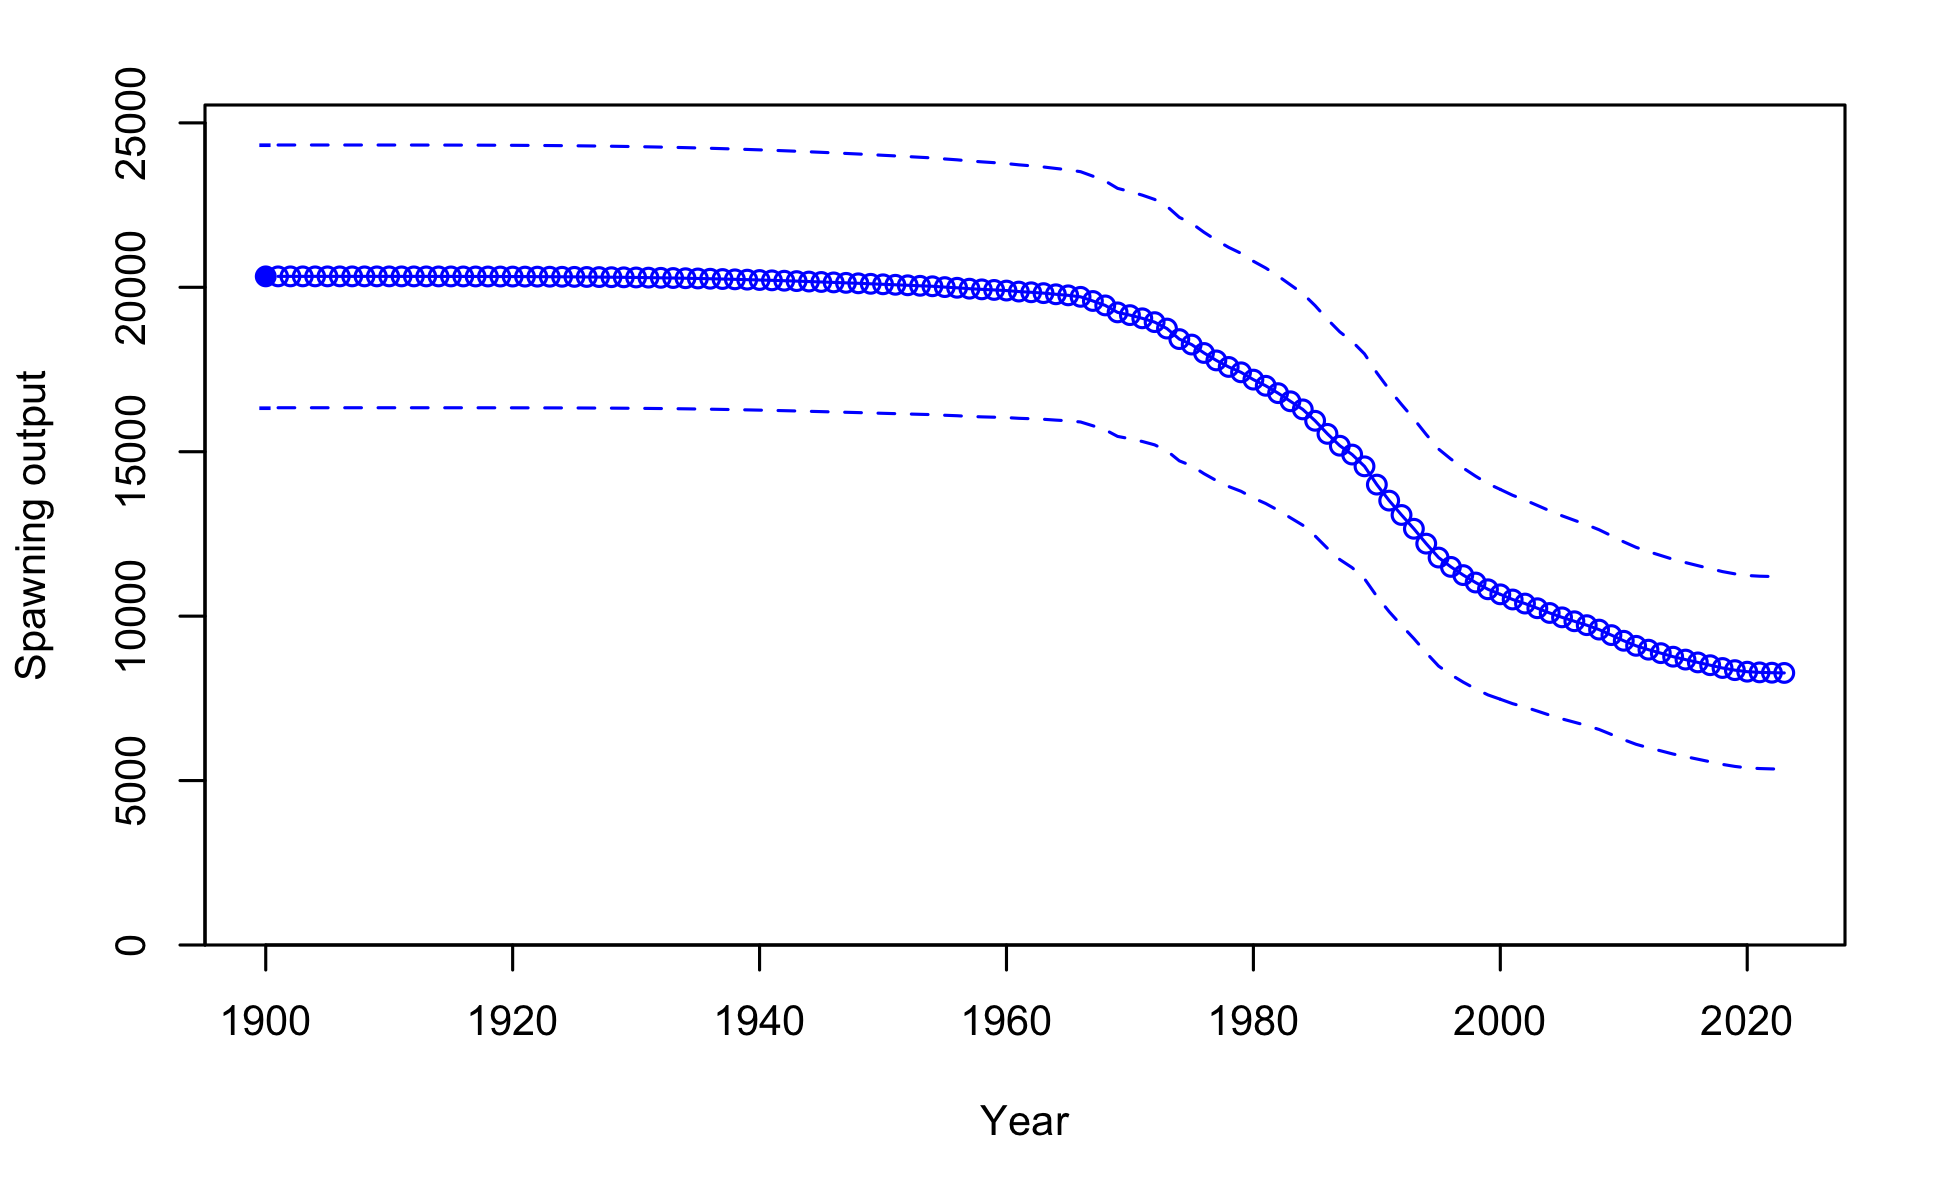
\includegraphics[width=1\textwidth,height=1\textheight]{/Users/jzahner/Desktop/Projects/shortspine_thornyhead_2023/doc/FinalFigs/Base/ts7_Spawning_output_with_95_asymptotic_intervals_intervals.png}
\caption{Estimated spawning output trajectory for shortspine thornyhead.\label{fig:ssb_trajectory}}
\end{figure}

\hypertarget{recruitment}{%
\subsection*{Recruitment}\label{recruitment}}
\addcontentsline{toc}{subsection}{Recruitment}

This assessment assumed a Beverton-Holt stock recruitment relationship. Steepness (the fraction of expected equilibrium recruitment associated with 20\% of equilibrium spawning biomass) was fixed at 0.7, slightly higher than what was assumed in previous assessments (h=0.60). The scale of the population is largely determined by the log of unfished recruitment (R0), which was estimated to be 9.354. This results in an unfished recruitment of 11,550,000 recruits (9,281,000--13,820,000). Recruitment deviations were estimated for the years 1901 through 2022, and ranged from -0.5 to 1.5 on the log scale. Estimated recruitments do not show high variability, and the uncertainty in each estimate is greater than the variability between estimates.

\begingroup\fontsize{10}{12}\selectfont
\begingroup\fontsize{10}{12}\selectfont

\begin{longtable}[t]{c>{\centering\arraybackslash}p{2.2cm}>{\centering\arraybackslash}p{2.2cm}>{\centering\arraybackslash}p{2.2cm}>{\centering\arraybackslash}p{2.2cm}}
\caption{\label{tab:rec}Estimated recent trend in recruitment and recruitment deviations and the 95\% confidence intervals (CI) from the base model.}\\
\toprule
Year & Recruitment & 95\% CI & RecDevs & RecDev 95\% CI\\
\midrule
\endfirsthead
\caption[]{\label{tab:rec}Estimated recent trend in recruitment and recruitment deviations and the 95\% confidence intervals (CI) from the base model. \textit{(continued)}}\\
\toprule
Year & Recruitment & 95\% CI & RecDevs & RecDev 95\% CI\\
\midrule
\endhead

\endfoot
\bottomrule
\endlastfoot
2013 & 6,024 & 2,469–14,698 & -0.439 & -1.352–0.474\\
2014 & 5,962 & 2,446–14,532 & -0.447 & -1.358–0.465\\
2015 & 5,954 & 2,438–14,542 & -0.446 & -1.360–0.468\\
2016 & 6,057 & 2,465–14,886 & -0.427 & -1.349–0.495\\
2017 & 5,836 & 2,385–14,279 & -0.462 & -1.379–0.454\\
2018 & 5,745 & 2,346–14,069 & -0.476 & -1.393–0.442\\
2019 & 8,863 & 3,557–22,086 & -0.064 & -1.003–0.874\\
2020 & 9,536 & 3,760–24,183 & -0.013 & -0.973–0.946\\
2021 & 10,335 & 3,984–26,811 & 0.044 & -0.943–1.032\\
2022 & 10,118 & 3,924–26,090 & 0.000 & -0.980–0.980\\
2023 & 10,117 & 3,924–26,086 & 0.000 & -0.980–0.980\\*
\end{longtable}
\endgroup{}
\endgroup{}

\begin{figure}
\centering
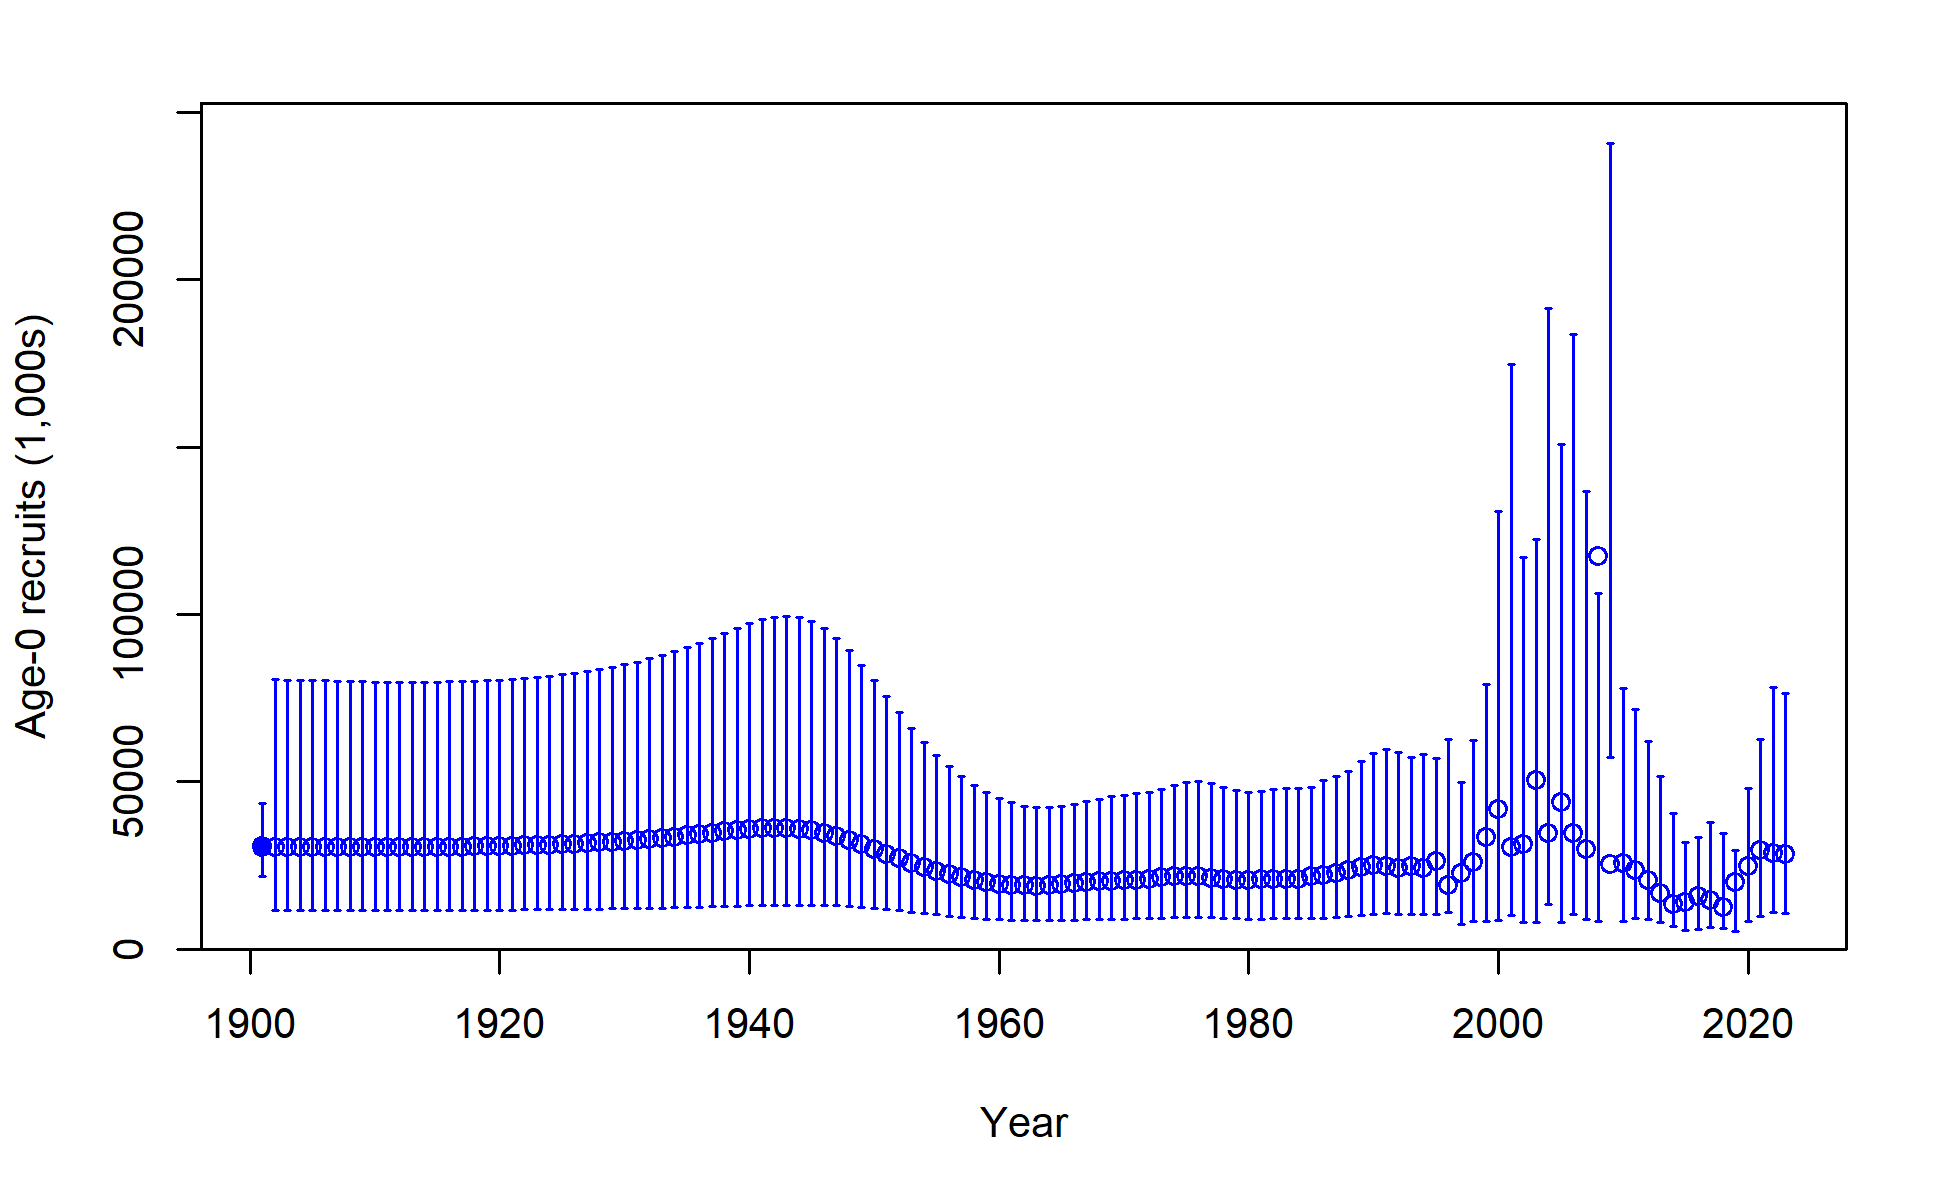
\includegraphics[width=1\textwidth,height=1\textheight]{/Users/jzahner/Desktop/Projects/shortspine_thornyhead_2023/doc/FinalFigs/Base/ts11_Age-0_recruits_(1000s)_with_95_asymptotic_intervals.png}
\caption{Estimated recruitment timeseries.\label{fig:rec_trajectory}}
\end{figure}

\hypertarget{exploitation-status}{%
\subsection*{Exploitation status}\label{exploitation-status}}
\addcontentsline{toc}{subsection}{Exploitation status}

The summary harvest rate (total catch divided by age-1 and older biomass) closely follows the landings trajectory. The harvest rates are estimated to have never exceeded 5\% and have remained below 2\% in the past decade. Expressing exploitation rates in terms of spawning potential ratio (SPR) indicates that the exploitation consistently exceeded the SPR50\% reference point from 1980-2018. However, the stock status is estimated to have never fallen below the B40\% management target, though the uncertainty interval around the 2023 estimate does encapsulate the B40\% target.

\begingroup\fontsize{10}{12}\selectfont
\begingroup\fontsize{10}{12}\selectfont

\begin{longtable}[t]{c>{\centering\arraybackslash}p{2.2cm}>{\centering\arraybackslash}p{2.2cm}>{\centering\arraybackslash}p{2.2cm}>{\centering\arraybackslash}p{2.2cm}}
\caption{\label{tab:spr}Estimated recent trend in the (1-SPR)/(1-SPR 50\%) where SPR is the spawning potential ratio the exploitation rate, and the  95\% intervals.}\\
\toprule
Year & (1-SPR)/(1-SPR 50\%) & 95\% CI & Exploitation Rate & 95\% CI\\
\midrule
\endfirsthead
\caption[]{\label{tab:spr}Estimated recent trend in the (1-SPR)/(1-SPR 50\%) where SPR is the spawning potential ratio the exploitation rate, and the  95\% intervals. \textit{(continued)}}\\
\toprule
Year & (1-SPR)/(1-SPR 50\%) & 95\% CI & Exploitation Rate & 95\% CI\\
\midrule
\endhead

\endfoot
\bottomrule
\endlastfoot
2013 & 1.25 & 1.03–1.47 & 0.0124 & 0.0084–0.0165\\
2014 & 1.12 & 0.90–1.34 & 0.0103 & 0.0069–0.0137\\
2015 & 1.15 & 0.92–1.37 & 0.0109 & 0.0073–0.0145\\
2016 & 1.19 & 0.96–1.42 & 0.0117 & 0.0078–0.0155\\
2017 & 1.23 & 1.00–1.46 & 0.0125 & 0.0083–0.0167\\
2018 & 1.09 & 0.86–1.32 & 0.0103 & 0.0069–0.0138\\
2019 & 0.95 & 0.73–1.17 & 0.0085 & 0.0056–0.0114\\
2020 & 0.66 & 0.48–0.84 & 0.0053 & 0.0035–0.0071\\
2021 & 0.59 & 0.43–0.76 & 0.0047 & 0.0031–0.0063\\
2022 & 0.64 & 0.47–0.81 & 0.0052 & 0.0034–0.0070\\*
\end{longtable}
\endgroup{}
\endgroup{}

\begin{figure}
\centering
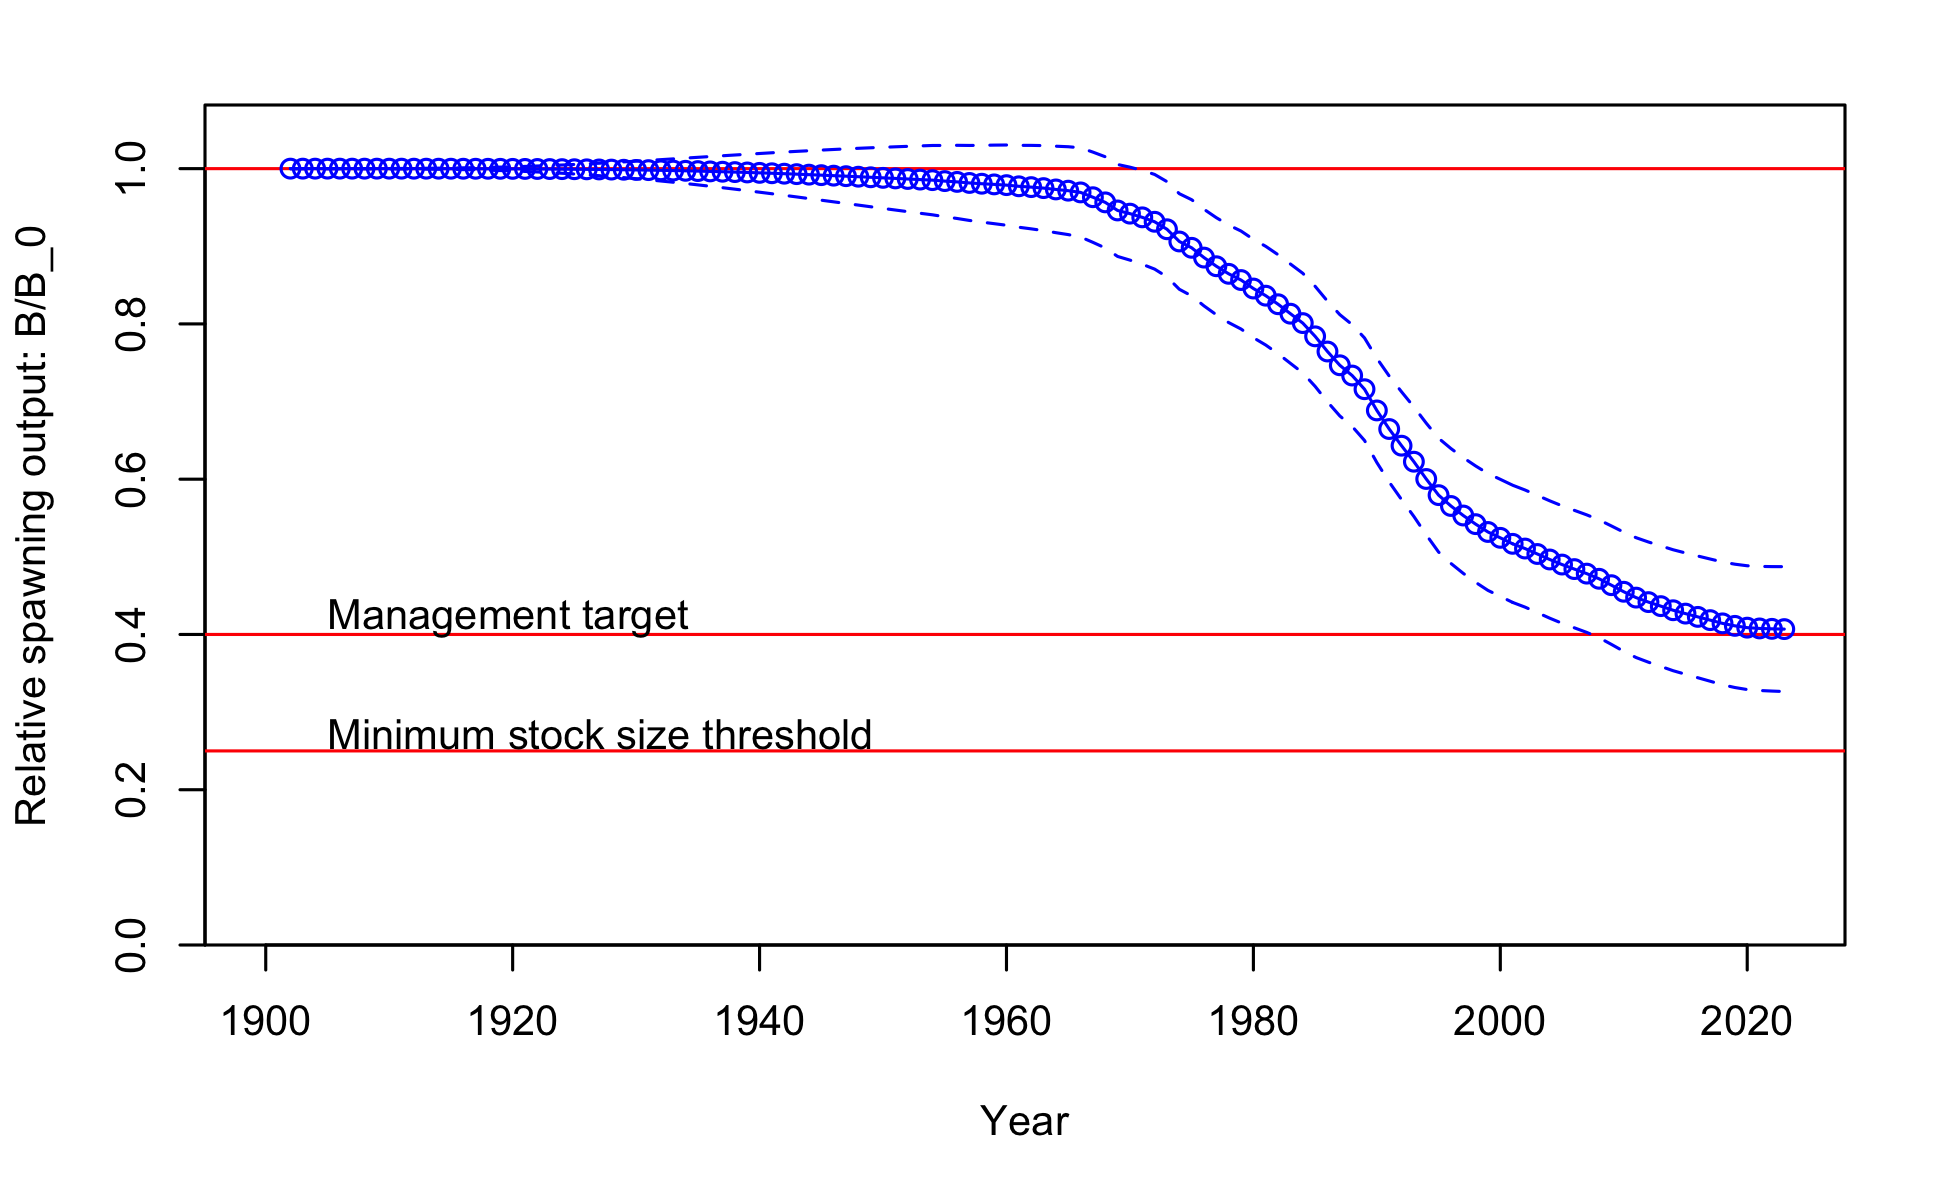
\includegraphics[width=1\textwidth,height=1\textheight]{/Users/jzahner/Desktop/Projects/shortspine_thornyhead_2023/doc/FinalFigs/Base/ts9_Relative_spawning_output_intervals.png}
\caption{Estimated relative spawning output trajectory for shortspine thornyhead.\label{fig:rel_ssb_trajectory}}
\end{figure}

\begin{figure}
\centering
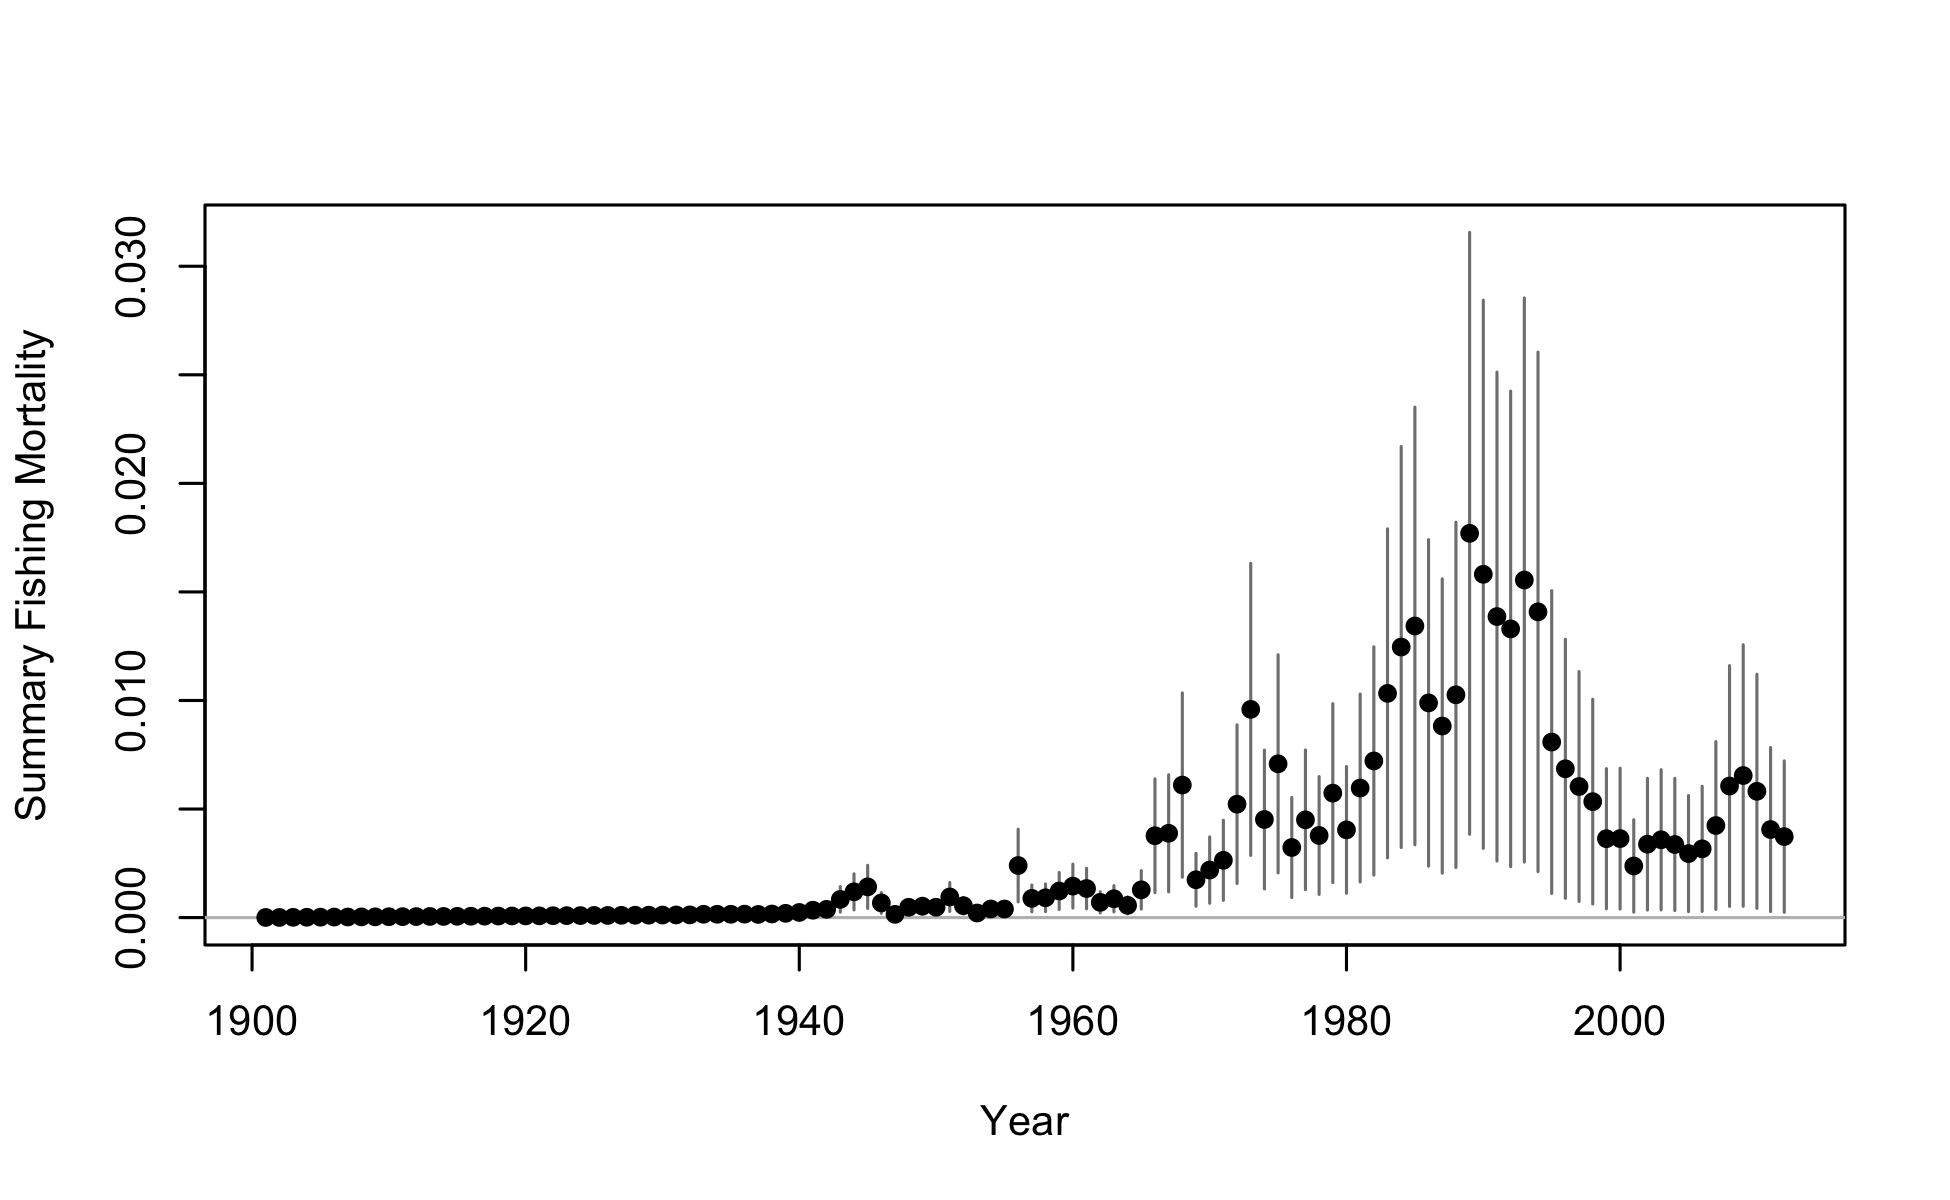
\includegraphics[width=1\textwidth,height=1\textheight]{/Users/jzahner/Desktop/Projects/shortspine_thornyhead_2023/doc/FinalFigs/Base/ts_summaryF.png}
\caption{Summary F rate.\label{fig:summary_f}}
\end{figure}

\begin{figure}
\centering
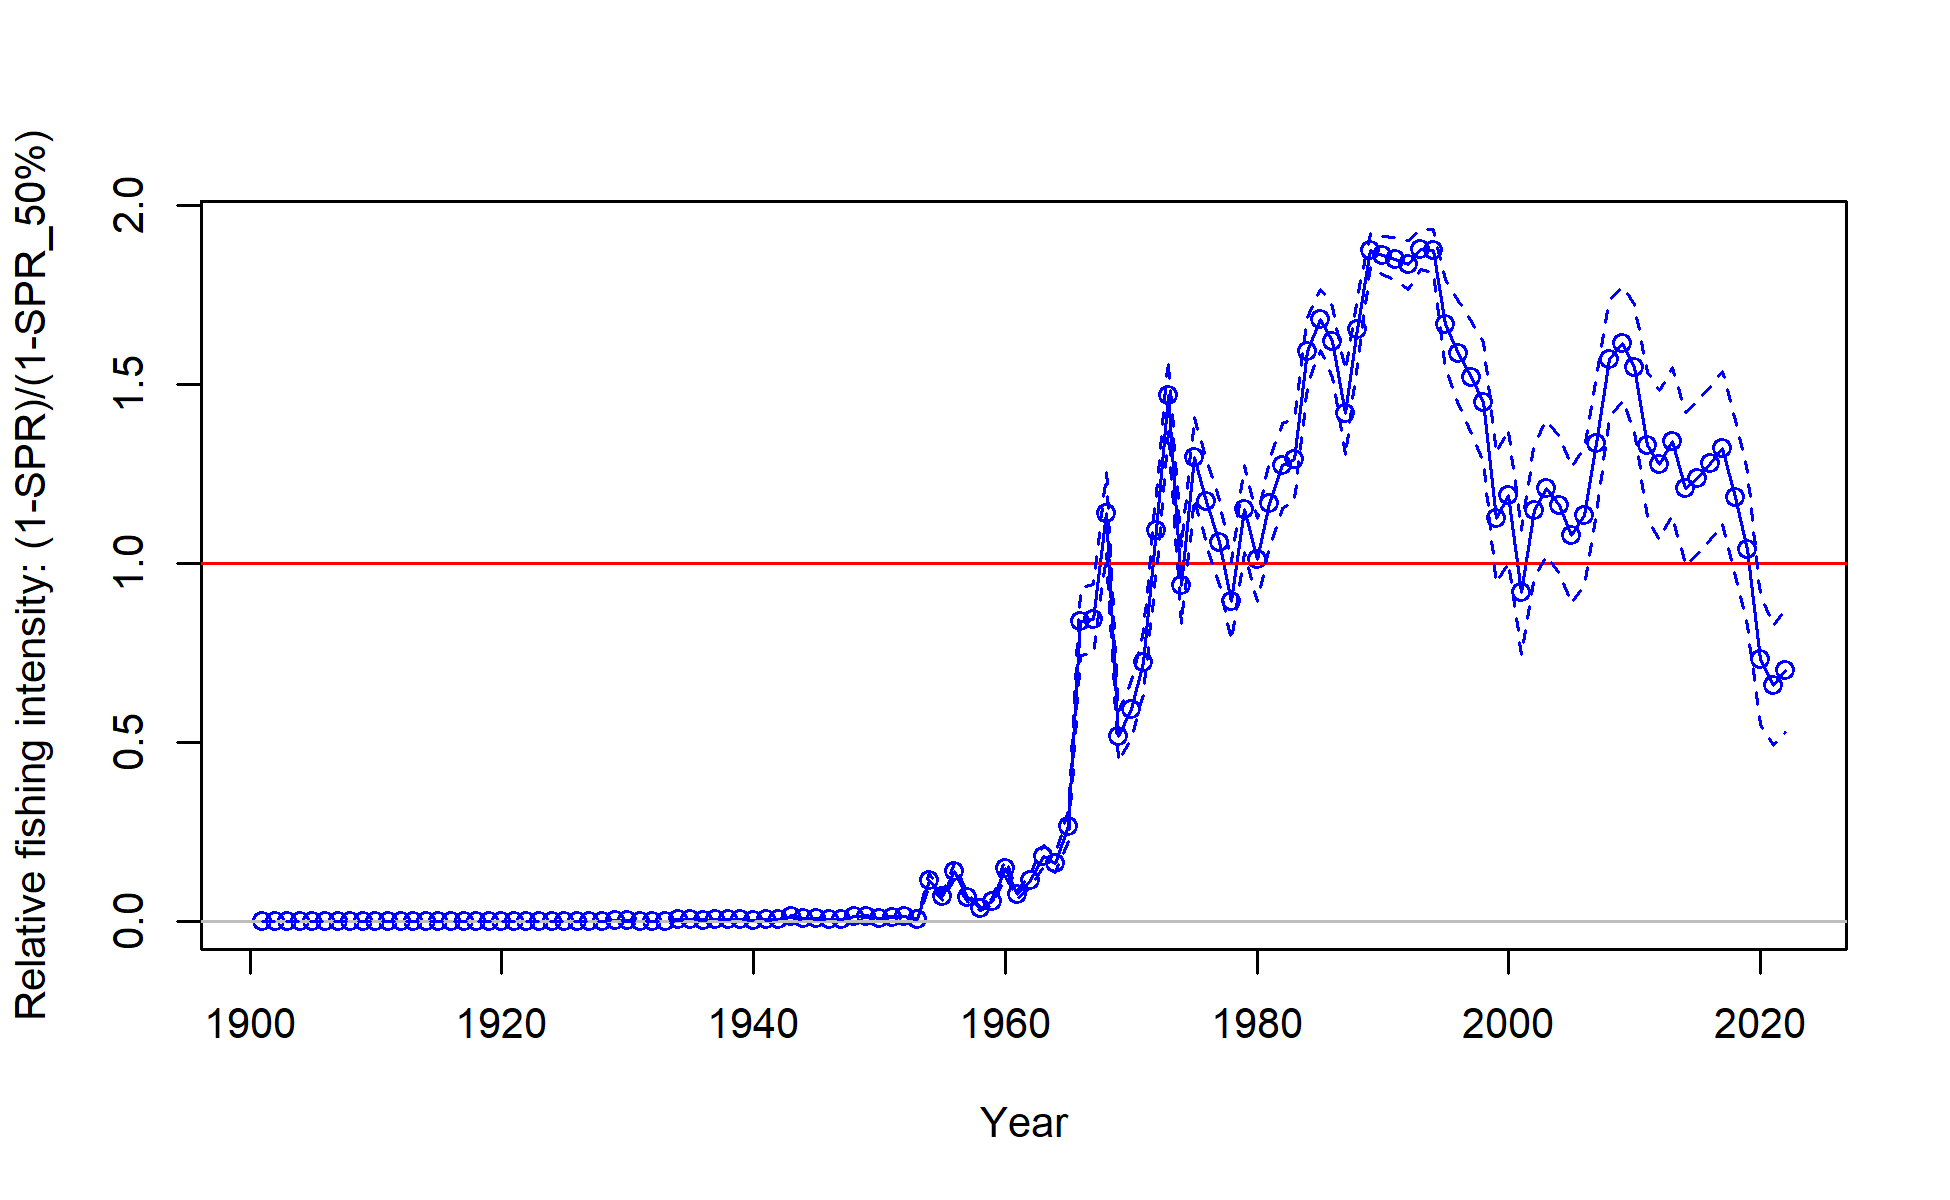
\includegraphics[width=1\textwidth,height=1\textheight]{/Users/jzahner/Desktop/Projects/shortspine_thornyhead_2023/doc/FinalFigs/Base/SPR3_ratiointerval.png}
\caption{Estimated spawning potential ratio.\label{fig:spr_trajectory}}
\end{figure}

\begin{figure}
\centering
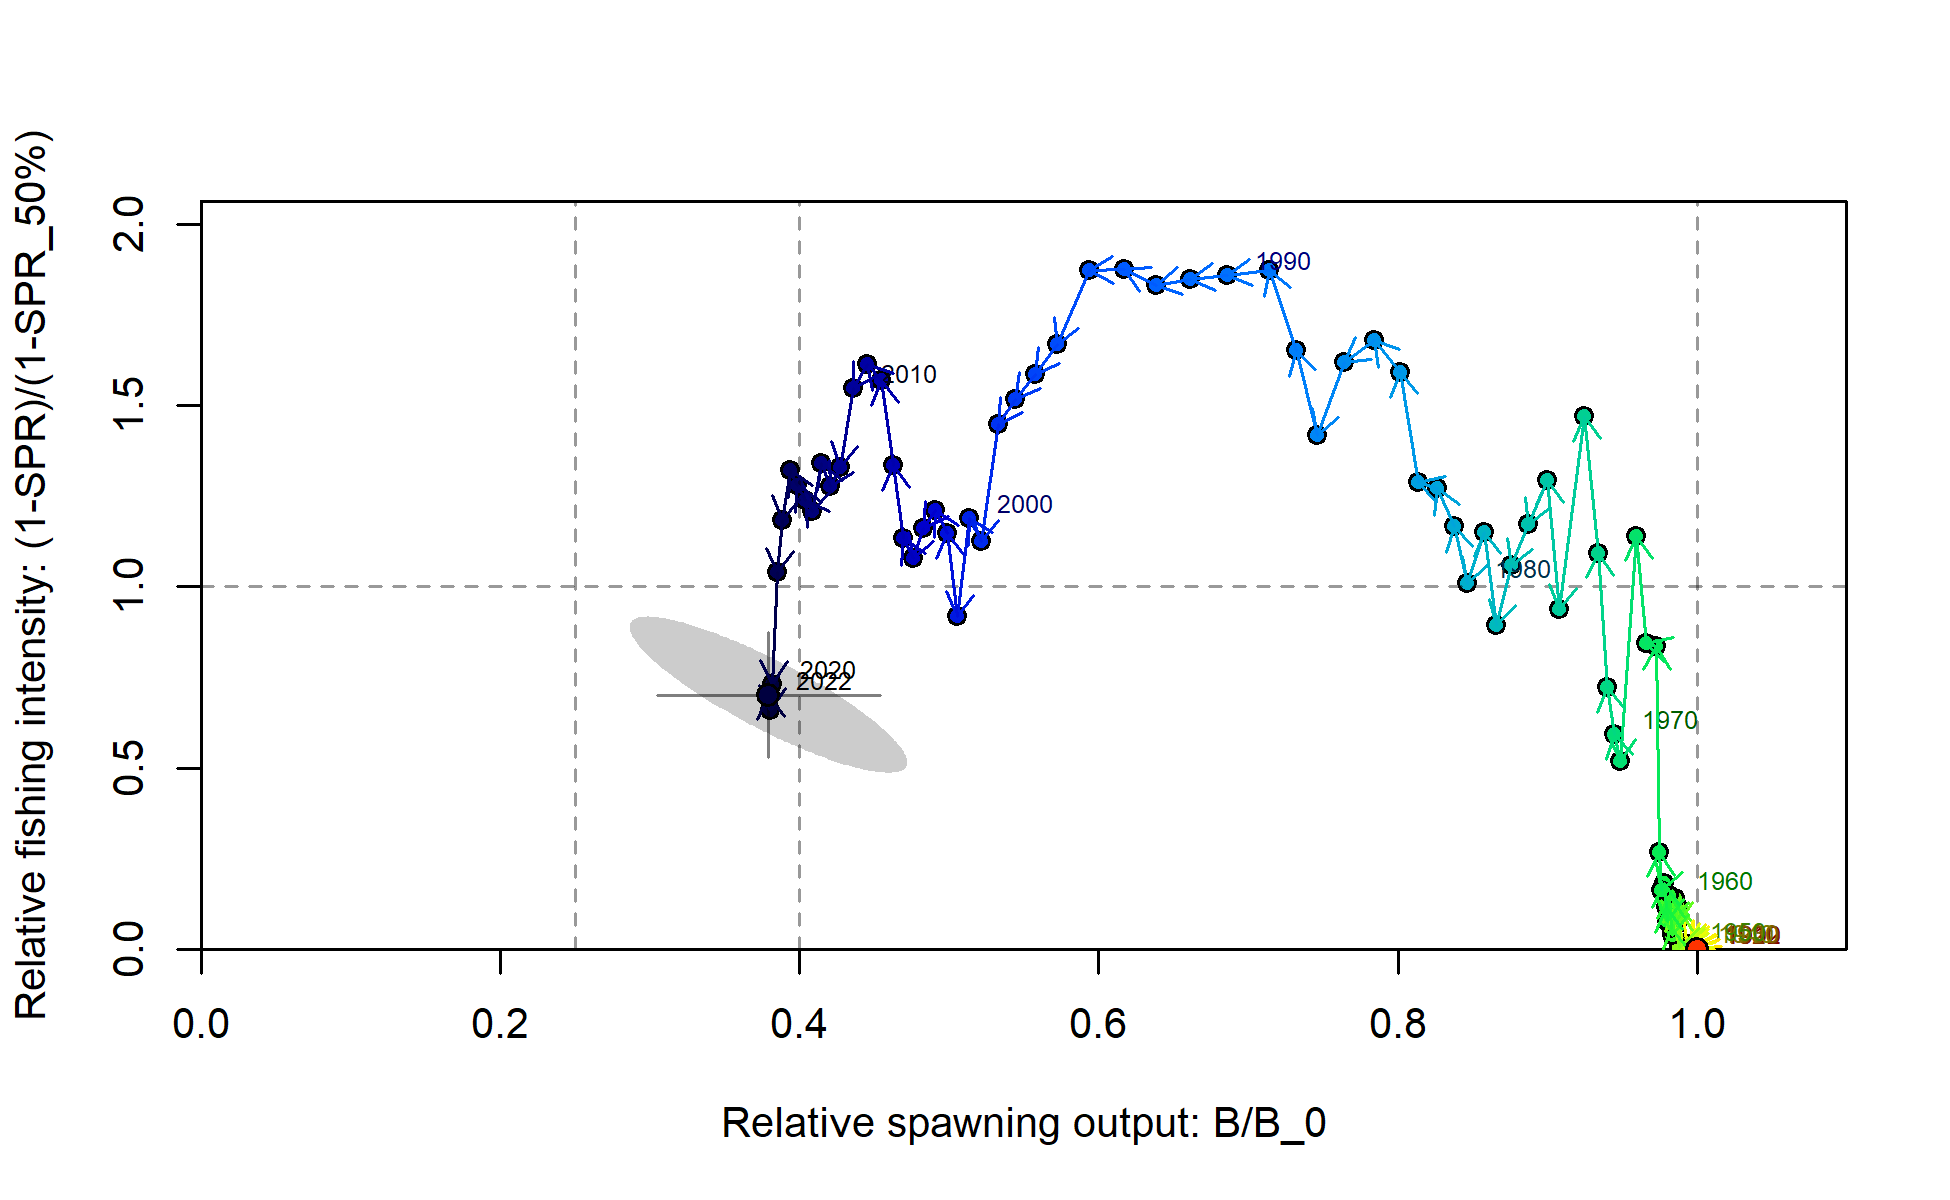
\includegraphics[width=1\textwidth,height=1\textheight]{/Users/jzahner/Desktop/Projects/shortspine_thornyhead_2023/doc/FinalFigs/Base/SPR4_phase.png}
\caption{Phase diagram.\label{fig:phase_diagram}}
\end{figure}

\hypertarget{ecosystem-considerations}{%
\subsection*{Ecosystem considerations}\label{ecosystem-considerations}}
\addcontentsline{toc}{subsection}{Ecosystem considerations}

Replace text with a summary of reviewed environmental and ecosystem factors that appear to be correlated with stock dynamics. These may include variability in they physical environment, habitat, competitors, prey, or predators that directly or indirectly affects the stock's status, vital rates (growth, survival, productivity/recruitment) or range and distribution. Note which, if any, ecosystem factors are used in the assessment and how (e.g., as background information, in data preparations, as data inputs, in decisions about model structure).

\hypertarget{reference-points}\), i.e., the \(B_{MSY}\) proxy and the equilibrium stock size that results from fishing at the default harvest rate, i.e., the \(F_{MSY}\) proxy. Include Table of estimated reference points for ssb, SPR, exploitation rate, and yield based on SSB proxy for MSY, SPR proxy for MSY, and estimated MSY values.

\hypertarget{management-performance}{%
\subsection*{Management performance}\label{management-performance}}
\addcontentsline{toc}{subsection}{Management performance}

Include Table of most recent 10 years of catches in comparison with OFL, ABC, HG, and OY/ACL values, overfishing levels, actual catch and discard. Include OFL (encountered), OFL (retained), and OFL (dead) if different due to discard and discard mortality.

\hypertarget{unresolved-problems-and-major-uncertainties}{%
\subsection*{Unresolved problems and major uncertainties}\label{unresolved-problems-and-major-uncertainties}}
\addcontentsline{toc}{subsection}{Unresolved problems and major uncertainties}

Major uncertainties in the model are centered around uncertainty in biological processes including growth, maturity, and mortality. The absence of reliable ageing methods for Shortspine thornyhead, particularly, makes it difficult to estimate growth and natural mortality. Sensitivities demonstrated that changes to the growth curve have large effects on the estimated stock status. Likelihood profiles over natural mortality demonstrate the model to be quite sensitive to its assumed value. There is insufficient information in the data to estimate mortality directly, constraining us to use meta-analyses or other mortality estimators, which frequently make use of aging information that is unavailable, and again, highly uncertain for shortspine thornyhead. Due to imperfect seasonal and spatial coverage of histological data for shortspine thornyhead, there is significant uncertainty about the shape of the species' maturity curve, though the model appears to be largely insensitive to variations in maturity.

This model fails to fully capture the observed increase in abundance seen in the WCGBTS index time series in 2021 and 2022. The model also fails to fully capture the peak of the length compositions for the Northern Trawl fleet, underestimating the number of mid-sized fish that the fleet takes \emph{(Figure XX)}. This underestimation appears to be consistent, particularly in the last 10 years \emph{(Figure XX)}, implying a possible recent change in selectivity.

\hypertarget{decision-table-and-projections}{%
\subsection*{Decision table and projections}\label{decision-table-and-projections}}
\addcontentsline{toc}{subsection}{Decision table and projections}

Replace text with projected yields (OFL, ABC, and ACL), spawning biomass, and stock depletion levels for each year. OFL calculations should be based on the assumption that future catches equal ABCs and not OFLs.

\hypertarget{scientific-uncertainty}{%
\subsection*{Scientific uncertainty}\label{scientific-uncertainty}}
\addcontentsline{toc}{subsection}{Scientific uncertainty}

Replace text with the sigma value and the basis for its calculation.

\hypertarget{research-and-data-needs}{%
\subsection*{Research and data needs}\label{research-and-data-needs}}
\addcontentsline{toc}{subsection}{Research and data needs}

Research and data needs for future assessments include the following:

\begin{enumerate}
\def\labelenumi{\arabic{enumi}.}
\tightlist
\item
  Research into ageing methods and availability of reliable age data would be valuable for future stock assessments. Otoliths have been collected in good quantities from the NWFSC survey, but there is currently no validated ageing method for Shortspine thornyhead.
\item
  More investigation into maturity of Shortspine thornyhead is necessary to understand the patterns in maturity observed in WCGBTS samples.
\item
  Information on possible migration of Shortspine thornyheads would be valuable for understanding stock dynamics. Analysis of trace elements and stable isotopes in shortspine otoliths may provide valuable information on the extent of potential migrations. Possible connections between migration and maturity could likewise be explored.
\item
  A greater understanding of the connection between thornyheads and bottom type could be used to refine the indices of abundance. Thornyheads are very well sampled in trawlable habitat, but the extrapolation of density to a survey stratum could be improved by accounting for the proportion of different bottom types within a stratum and the relative density of thornyheads within each bottom type.
\item
  Additional investigation into spatial stock structure could be valuable for determining whether future assessments should develop a spatial assessment model, or if shortspine thornyhead should be assessed at distinct spatial scales in the future.
\end{enumerate}

\pagebreak
\setlength{\parskip}{5mm plus1mm minus1mm}
\pagenumbering{arabic}
\setcounter{page}{1}
\renewcommand{\thefigure}{\arabic{figure}}
\renewcommand{\thetable}{\arabic{table}}
\setcounter{table}{0}
\setcounter{figure}{0}

\hypertarget{introduction}{%
\section{Introduction}\label{introduction}}

\hypertarget{basic-information}{%
\subsection{Basic Information}\label{basic-information}}

This assessment reports the status of shortspine thornyhead (\emph{Sebastolobus alascanus}) off the US West coast using data through xxxx.

Shortspine Thornyhead (\emph{Sebastolobus alascanus}) are found in the waters off the West Coast of the United States from northern Baja California to the Bering Sea at depths of 20 meters to over 1,500 meters. The majority of the spawning biomass occurs in the oxygen minimum zone between 600 and 1,400 meters. The distribution of the smallest shortspine thornyhead suggests that they tend to settle at around 100--400 meters and are believed to have ontogenetic migration down the slope, although large individuals are found across the depth range. Higher densities (kg/ha) of shortspine thornyhead occur in shallower areas (under 500 meters) off Oregon and Washington, whereas in California, they occur in deeper areas (\textbf{above x meters;} Figure \ref{fig:stock-map}).

Despite variation in density across the coast, shortspine thornyheads are present in almost all trawlable areas below 500 meters. They are caught in 91\% of trawl survey hauls deeper than 500 m and \textbf{XX\%} of commercial bottom trawl hauls deeper than 500m. Camera-tows show that thornyheads are spaced randomly across the sea floor, indicating a lack of schooling and territoriality (Wakefield 1990; Du Preez and Tunnicliffe 2011).

\hypertarget{stock-structure}{%
\subsection{Stock Structure}\label{stock-structure}}

\textbf{NOTE: This section was added.}

Genetic studies of stock structure show few genetic differences among shortspine thornyhead along the Pacific coast, and thus do not suggest separate stocks Stepien (1995). Stepien (1995) suggested that there may be a separate population of shortspine thornyhead in the isolated area around Cortes Bank off San Diego, California. Stepien (1995) also pointed out that juvenile dispersion might be limited in the area where the Alaska and California currents split, which occurs towards the northern boundary of the assessment area, near 48° N.

Stepien et al. (2000), using a more discerning genetic material (mtDNA), found evidence of a pattern of genetic divergence in shortspine thornyhead corresponding to geographic distance. However, this study, which included samples collected from southern California to Alaska, did not identify a clear difference between stocks even at the extremes of the range. No such pattern was seen in longspine thornyhead, which suggests that the shorter pelagic stage (\textasciitilde1 yr vs.~\textasciitilde2 yrs) of shortspine thornyhead may contribute to an increased genetic separation with distance.

Dorval et al. (2022) applied otolith microchemistry to immature fish to redefine population structure of shortspine thornyhead on the west coast. Their results indicate that the population of immature shortspines belongs to two distinct groups distributed north and south of Cape Mendocino.

\hypertarget{life-history}{%
\subsection{Life History}\label{life-history}}

Shortspine Thornyheads along the West Coast spawn pelagic, gelatinous floating egg masses between December and May (Wakefield 1990; Erickson and Pikitch 1993; Pearson and Gunderson 2003). Cooper et al. (2005) and Pearson and Gunderson (2003) found no evidence for batch spawning in this species on the West Coast, but more recent histological examination of ovaries suggest that some shortspine thornyhead can be batch spawners with two to three batches developing simultaneously (Melissa Head, \gls{nwfsc}, pers. comm.). Juveniles settle at around 1 year of age (22- 27 mm in length), likely in the range of 100-200 m (Vetter and Lynn 1997), and migrate down the slope with age and size, although large individuals are found across the depth range.

Shortspine Thornyhead are notoriously challenging to age, and a recent age validation study using 14C bomb radiocarbon was inconclusive (Kastelle et al. 2020). However, best available data suggests that the shortspine thornyhead life span may exceed 100 y (Butler 1995; Kline 1996). Estimates of natural mortality for shortspine thornyhead range from 0.013 (Pearson and Gunderson 2003) to 0.07 (Kline 1996). However, Pearson and Gunderson's estimate is based upon a regression model, using the gonadosomatic index as a proxy. Butler (1995) estimated M to be 0.05 based upon a maximum lifespan of 100 years for shortspine thornyhead. Butler (1995) also suggested that M may be lower for older, larger shortspine thornyhead residing in the oxygen minimum zone due to lack of predators. All estimates of M for thornyheads are highly uncertain.

Shortspine Thornyhead grow very slowly and may continue growing throughout their lives, reaching maximum lengths of over 70 cm. Females grow to larger sizes than males. Maturity in females has been estimated as occurring near 18 cm, with fish transitioning from immature to mature within a relatively narrow range of sizes between 15 and 20 cm Pearson and Gunderson (2003). However, more recent histological data collected in the \gls{s-wcgbt} and analyzed using current best practices suggests that functional maturation, which accounts for abortive maturation and skip spawning, occurs over a broader spectrum of sizes between 10 and 55 cm (length-at-50\% maturity, L50 =31.4; personal communication, Melissa Head, \gls{nwfsc}, pers. comm.).

\hypertarget{ecosystem-considerations-1}{%
\subsection{Ecosystem Considerations}\label{ecosystem-considerations-1}}

Shortspine Thornyheads have historically been caught alongside longspine thornyheads in a \gls{dts}. Other groundfishes that frequently co-occur in deep waters include a complex of slope rockfishes, Rex sole, longnose skate, roughtail skate, Pacific grenadier, giant grenadier, and Pacific flatnose. Non-groundfish species such as Pacific hagfish and a diverse complex of eelpouts also co-occur with shortspine thornyhead.

Shortspine Thornyheads typically occur in shallower water than the shallowest longspine thornyheads, and migrate to deeper water as they age. The majority of spawning shortspine thornyheads occur between 600 and 1,400 meters, where longspine thornyheads are most abundant (Jacobson and Vetter 1996; Bradburn et al. 2011). When shortspine thornyheads have reached a depth where they overlap with longspine thornyheads, they are typically larger than the largest longspine thornyheads.

Species distribution models developed by Liu et al. (in press) suggest that expected environmental changes over the next decades will lead to a decline in shortspine and increase in longspine abundance. Shortspine Thornyheads are also projected to shift offshore, into deeper waters, potentially decreasing their availability in fisheries. To date, shortspine thornyheads have been observed by cameras below the 1280 meter limit of the current fishery and survey, but their distribution, abundance, and ecosystem interactions in these deep waters are relatively unknown. Thornyheads spawn gelatinous masses of eggs which float to the surface, which may represent a significant portion of the upward movement of organic carbon from the deep ocean (Wakefield 1990).

Shortspine Thornyhead diet composition, as derived from stomach content collection in the 1980s and 1990s, varied by year (Bizzarro et al. 2023). In some years their diet consisted primarily of invertebrate species including pandalid shrimp, pink shrimp, and Tanner crab, while in others their stomach content was dominated by finfish species such as Pacific cod and Pacific Hake. As prey themselves, shortspine thornyheads were only found in the stomachs of other species in two years, 1991 and 1992 as recorded in the \gls{cctd}, where shortspine thornyhead occurred in sablefish, Pacific hake, and other shortspine thornyhead stomachs (Bizzarro et al. 2023).

\hypertarget{historical-and-current-fishery-information}{%
\subsection{Historical and Current Fishery Information}\label{historical-and-current-fishery-information}}

Thornyhead harvest has experienced fluctuations over time due to increased depth range of the fisheries, variable markets, and changes in fisheries management. In the early 1900's, landings were minimal because there were few markets for thornyheads and relatively little trawling at depths where the majority of thornyheads occur. Beginning in the 1930s, thornyhead landings increased as they were landed as incidental catch in the California sablefish fishery. The first significant market for thornyheads began in northern California in the early 1960s, when larger (30-35 cm) thornyhead were sold as ``ocean catfish.'' By the early 1980s, the minimum marketable size decreased to 25 cm, and in the late 1980s a market for small thornyheads (\textasciitilde20 cm) developed due to the depletion of a related species (\emph{Sebastolobus machrochir}) off the coast of Japan. The fishery moved into deeper waters with the demand for smaller thornyheads and began catching more longspine thornyheads. This is reflected in the changes in proportion of shortspine to total thornyheads through time, which decreased from around 90\% in 1981 to 40\% in 1994 Figure \ref{fig:thornyhead-ratio}.

Landings of shortspine thornyheads off the coast of California peaked around 3,500 mt in 1989, and have exceeded those from further north in most years (Figure \ref{fig:catch_hist}). In the northern area off of Oregon and Washington, the fishery grew in the early 1980s, with landings peaking in 1991 at around 2200 mt.

Non-trawl landings of shortspine thornyheads were relatively low prior to the mid-1990s, at which point non-trawl landings, dominantly longline, in California began to increase steadily from less than 5 mt in 1994 to 237 mt in 2011. The increase in non-trawl landings was driven by the development of live-fish markets for thornyheads and the fact that ex-vessel prices associated with the non-trawl landings are much higher than those for the trawl fishery.

\textbf{Nominal prices for line-caught shortspine thornyhead increased steadily from \textdollar 0.69/lb in 1993 to \textdollar 3.81/lb in 2008, and have remained near or above that level since.} Citation?

Trawl prices, on the other hand, changed from \textdollar 0.46/lb to \textdollar 0.72/lb in the same period, although, when Japanese demand was strong they were between \textdollar 0.80 and \textdollar 1.06/lb. In contrast, non-trawl landings of shortspine in Washington and Oregon have remained below the estimated peak of 54 mt in 1991.

The foreign fishery off of the West Coast is estimated to have caught approximately 7,400 mt of shortspine thornyhead during the 11 year period from 1966-1976 (Rogers 2003), which is on the order of the estimate of domestic catch (\textasciitilde8,600 mt) during that same period.

\textbf{Management measures} have contributed to a decline in coastwide landings from an estimated peak of 4,815 mt in 1989 to between 1,000 and 2,000 mt per year from 1995 through 1998. Landings fell below 1,000 mt per year from 1999 through 2006, then rose to 1,531 in 2009 and have declined since \textbf{(Table X)}.

In 2011, the west coast trawl fishery was rationalized, with the introduction of the Individual Fishing Quota (IFQ) Program. In order to provide more flexibility for fishers on the west coast, NOAA Fisheries implemented the West Coast Groundfish Trawl Fishery Catch Share Program, which allows for the division of catch allocated to the trawl fishery into shares controlled by individuals or cooperatives (West Coast Regional Office n.d.). All vessels that participate in the IFQ program are required to have 100\% observer coverage at all times the vessels are at sea.(West Coast Regional Office n.d.)

\hypertarget{summary-of-management-history-and-performance}{%
\subsection{Summary of Management History and Performance}\label{summary-of-management-history-and-performance}}

Beginning in 1989, both thornyhead species were managed as part of a \gls{dts}. In 1991, the \gls{pfmc} adopted separate \gls{abc} levels for thornyheads and catch limits were imposed on the thornyhead complex. \gls{hg} were instituted in 1992 along with an increase in the minimum mesh size for bottom trawl fisheries. In 1995 separate landing limits were placed on shortspine and longspine thornyheads and trip limits became more restrictive. Trip limits (predominantly 2-month limits on cumulative vessel landings) have often been adjusted during the year since 1995 in order to not exceed the \gls{hg} or \gls{oy}. At first, the HG for shortspine thornyhead was set higher than the \gls{abc} (1,500 vs.~1,000 mt in 1995-1997) in order to allow a greater catch of longspine thornyhead, which was considered relatively undepleted. In 1999 the \gls{oy} was set at less than 1,000 mt and remained close to that level through 2006. As a result of the 2005 shortspine assessment, catch limits increased to about 2,000 mt per year and have remained near that level \textbf{to the present.}

Since early 2011, trawl harvest of each thornyhead species has been managed under the PFMC's catch share, or \gls{ifq}, program. Whereas the trip limits previously used to limit harvest restricted only the amount of fish each vessel could land, individual vessels fishing under the catch-share program are now held accountable for all of the quota-share species they catch.

\textbf{Landings of shortspine thornyhead have been below the catch limits since 1999. The estimated total catch, including discards, has likewise remained below the limit during this period.}

\hypertarget{foreign-fisheries}{%
\subsection{Foreign Fisheries}\label{foreign-fisheries}}

The \gls{afsc} conducts assessments of thornyheads as a mixed stock complex, including shortspine and longspine thornyheads. Results of the 2022 Alaska Thornyhead complex assessment suggest that thornyheads are not being subjected to overfishing (Echave et al. 2022).

\hypertarget{data}{%
\section{Data}\label{data}}

Data comprise the foundational components of stock assessment models. The decision to include or exclude particular data sources in an assessment model depends on many factors. These factors often include, but are not limited to, the way in which data were collected (e.g., measurement method and consistency); the spatial and temporal coverage of the data; the quantity of data available per desired sampling unit; the representativeness of the data to inform the modeled processes of importance; timing of when the data were provided; limitations imposed by the Terms of Reference; and the presence of an avenue for the inclusion of the data in the assessment model. Attributes associated with a data source can change through time, as can the applicability of the data source when different modeling approaches are explored (e.g., stock structure or time-varying processes). Therefore, the specific data sources included or excluded from this assessment should not necessarily constrain the selection of data sources applicable to future stock assessments for shortspine thornyhead. Even if a data source is not directly used in the stock assessment they can provide valuable insights into biology, fishery behavior, or localized dynamics.

Data from a wide range of programs were available for possible inclusion in the current assessment model. Descriptions of each data source included in the model (Figure \ref{fig:assessment_data_timeseries}) and sources that were explored but not included in the base model are provided below. Data that were excluded from the base model were explicitly explored during the development of this stock assessment or have not changed since their past exploration in a previous shortspine thornyhead stock assessment. In some cases, the inclusion of excluded data sources were explored through sensitivity analyses.

\hypertarget{fishery-dependent-data}{%
\subsection{Fishery-Dependent Data}\label{fishery-dependent-data}}

\hypertarget{catch-history}{%
\subsubsection{Catch History}\label{catch-history}}

\Gls{pacfin} data from 1981-present was used to estimate landings in the North (Oregon and Washington) and South (California) by gear type (Trawl and Non-Trawl) (Figure \ref{fig:catch_hist}) All landings reported for the shortspine thornyhead and nominal shortspine thornyhead categories were considered shortspine thornyhead, whereas landings categorized as unidentified thornyheads were split between longspine thornyhead and shortspine thornyhead by the ratio of identified longspine and shortspine landings for each year-state-gear combination. The values of this ratio for each state and gear-type from 1981-2023 are shown in Figure \ref{fig:thornyhead-ratio}.

Catches prior to 1981 are based on historical reconstructions provided by the respective states and a reconstruction of foreign fleet catch. Oregon landings for 1892-1986 are provided by ODFW and outlined in Karnowski et al. (2014) shortspine thornyhead landings are not present in the \gls{pacfin} data for Oregon for the years 1981-1986 and the state reconstruction is used for this period instead. Washington landings for 1954-1980 are provided by WDFW. Landings prior to the beginning of this data are assumed to be zero. California landings are provided by CDFW and SWFSC, and consist of California commercial data for 1969-1980, and a catch reconstruction documented by Ralston et al. (2010) for 1934-1968. As in the two previous assessments, catch data from Rogers (2003) is used to account for catches by foreign fleets during the years 1966-1976. Foreign catch in the Monterey and Eureka \gls{inpfc} areas is attributed to the Southern Trawl fleet, while foreign catch in Columbia and Vancouver areas is attributed to the Northern Trawl fleet, as was the case in the 2013 assessment.

For historical catches prior to 1981, all shortspine thornyhead, nominal shortspine, and unidentified thornyhead landings in the state catch reconstructions are considered shortspine thornyhead. Neither California reconstructions prior to 1978, nor the Karnowski et al. (2014) reconstruction for Oregon, distinguish between shortspine and longspine thornyhead species. It is possible that assigning all thornyhead landings to shortspine overestimates shortspine landings, however, the overwhelming majority of thornyhead landings were shortspine until the late 1980s when vessels began to move into deeper waters and a distinct fishery targeting longspine thornyhead developed (Hamel 2005; Karnowski et al. 2014).

This treatment of unassigned thornyhead landings differs from the 2005 and 2013 assessments. The 2005 assessment did not have access to the historical reconstructions used here, and instead imputed shortspine landings as 30\% of annual sablefish landings for the years 1901-1961. The 2013 assessment used the same imputed values as the 2005 assessment, but also conducted a sensitivity analysis in which all unassigned thornyheads in historical catch were considered shortspine thornyhead. Stock abundance estimates were found to be largely insensitive to which reconstructions were used (Taylor and Stephens 2013). The imputed historical values used for the 2005 and 2013 assessments will continue to be included as a sensitivity analysis here. Landings after 1961 remain very similar to the landings used in the 2013 assessment (Figure \ref{fig:catch_hist}).

\hypertarget{discards-and-retention}{%
\subsubsection{Discards and retention}\label{discards-and-retention}}

Predicted discards were based on estimated retention and selectivity for each fleet and are shown in Figure \ref{fig:disc_hist}. Discards were informed by four data sources covering three different periods. Data sets included, 1) Pikitch et al. (1988) Discard and Mesh Studies, used to estimate both discard rates and length composition of the northern trawl fleet between 1985 and 1987 (J. R. Wallace, pers. comm.), 2) the TEST \gls{edcp} covering 1995-1999, which only informed discard rates of the northern trawl fleet, 3) the \gls{wcgop}, which provided discard rates, length composition, and individual average weight for years between 2002 and 2021 for all fleets, and 4) the \gls{gemm} data set, covering the same period and completing the \gls{wcgop} with catch-share participation information and estimates of discard survival rates.

While the estimates from the first two data sets were directly integrated into the model, fleet discard rates after 2011 were available separately for catch-share and non-catch-share programs. Final fleet-specific discard rates were thus computed as the average \gls{wcgop} discard rate weighted by the relative proportion of total landings belonging to the catch-share and non-catch-share, respectively. (Figure \ref{fig:disc_rates_WCGOP}). Regardless of the type of data, all estimates derived from these data sets had associated uncertainty accounting for the variability observed within the sample of hauls and fishing trips of each fleet. WCGOP-derived discard rates are an exception as, after the catch share program was initiated in 2011, 100\% of hauls from catch share fleets were observed., while non-catch share vessels were only partially covered \emph{\emph{(cite)}}.

The discard data sources were the same as those used in the 2013 assessment. The main improvements are the increased representativity of all 4 fleets (11 more years) and more accurate estimates of discard rates from \gls{edcp}that were not ready at the time of the previous assessment. Last, some errors in the previous assessment were corrected regarding the weight units considered for the average individual weight (\gls{wcgop} provides weight as pounds and not as kg).

\hypertarget{fishery-length-compositions}{%
\subsubsection{Fishery Length Compositions}\label{fishery-length-compositions}}

Commercial fishery length-composition data were obtained from \gls{pacfin} for 1978-2023. Due to variations in sampling effort and because the number of fish sampled by port samplers is not proportional to the amount of landed catch in each trip, the observed length data were expanded using the following algorithm using the PacFIN.Utilities package in R:

\begin{enumerate}
\def\labelenumi{\arabic{enumi}.}
\tightlist
\item
  Length data were acquired at the trip level by sex, year and state.
\item
  The raw numbers in each trip were scaled by a per-trip expansion factor calculated by dividing the total weight of trip landings by the total weight of the species sampled.
\item
  A per-year, per-state expansion factor was computed by dividing the total weight of state landings by the total weight of the species sampled for length in the state.
\item
  The per-trip expanded numbers were multiplied by the per-state expansion factor and summed to provide the coast-wide length-frequency distributions by year.
\end{enumerate}

Only randomly collected samples were used. The sample sizes associated with the length compositions from the fishing fleets are shown in \emph{\emph{Table X (landings)}} and \emph{\emph{Table X (discards)}}. Length samples from the Trawl North fleet in 1980, 1994, and 1995 showed a very different pattern than the surrounding years. The effective sample sizes for these years were substantially lower than other years (Neff \textless{} 15), so the observed differences are likely due to non-representative sampling.

Input sample sizes \{N\_\{input\}\} for fishery length frequency distributions by year were calculated as a function of the number of trips and number of fish via the Stewart Method (Stewart, pers.com): \begin{align*}{N_{input} = N_{trips} + 0.138N_{fish}}\qquad\text{ when }\frac{N_{fish}}{N_{trips}}<44 \\
{N_{input} = 7.06N_{trips}}\qquad\qquad\qquad\text{ when }\frac{N_{fish}}{N_{trips}}\ge 44 \end{align*} The method is based on analysis of the input and model-derived effective sample sizes from west coast groundfish stock assessments. A piece-wise linear regression was used to estimate the increase in effective sample size per sample based on fish-per-sample and the maximum effective sample size for large numbers of individual fish.

All length data from commercial fisheries included in the model with sexes combined. This avoids the possibility of bias due to difficulty in sex determination of thornyheads.

\hypertarget{age-compositions}{%
\subsubsection{Age Compositions}\label{age-compositions}}

No age composition data was used for this assessment because thornyheads have proven very difficult to age (P. MacDonald, pers. comm.). Even in directed studies such as those done by Kline (1996) and Butler (1995), there are large inter-reader differences, and a second reading by the same ager can produce a markedly different result. Kline (1996) reported only about 60\% of the multiple reads were within 5 years of each other, and inter-reader differences were as large as 24 years for a sample of 50 otoliths. No production ageing of thornyheads is undertaken at this time for the west coast, although shortspine thornyhead otoliths are routinely collected in the NWFSC trawl survey.

\hypertarget{fishery-independent-data}{%
\subsection{Fishery-Independent Data}\label{fishery-independent-data}}

Four trawl surveys have been conducted on the U.S. west coast over the past four decades.

\hypertarget{section}{%
\subsubsection{\texorpdfstring{\acrlong{s-tri}}{}}\label{section}}

The \gls{afsc} conducted a triennial groundfish trawl survey (the ``triennial'' survey) on the continental shelf from 1977 to 2001, although the 1977 survey had incomplete coverage and is not believed to be comparable to the later years. A final survey was conducted in 2004 by the \gls{nwfsc} using the same survey design. In 1995, the timing of the survey shifted so that instead of occurring between mid-July and late September, it was conducted from early June through mid-August. The years 1980--1992 had a maximum depth of 366 m, while from 1995 onward, the maximum depth was extended to 500 m. The shallow limit of the survey was 55 m in all years, but for purposes of computing indices, only tows deeper than 100 m were used as shortspine thornyhead are rarely seen at shallower depths. The triennial survey consists of 9 data points, from surveys operating every third year from 1980--2004.

For some species, the shift in timing between the 1992 and 1995 surveys would be expected to influence their catchability, availability, or distribution. However, thornyheads are believed to be sedentary enough that the change in timing would not be as influential. On the other hand, the increase in depth is expected to significantly increase the range of shortspine thornyhead habitat covered by the survey. In the 2013 assessment, the triennial survey was split into two-time series, separated by the 366 m depth contour, in order to preserve a time series of maximum length while eliminating the influence of the increased depth range. The first time series, ``AFSC Triennial Shelf Survey 1,'' consists of 9 data points spanning the range 1980--2004 and covering the depths 100--366 m. The second, ``AFSC Triennial Shelf Survey 2,'' consists of 4 data points spanning 1995--2004 and covering depths 366--500 m. This second time series is recognized as providing little information about stock status due to the limited number of points and depth range, but there was no compelling reason to exclude it from the assessment. However, in contrast to the 2013 assessment, this assessment will treat the triennial survey as a single time series for constructing the geostatistical model-based indices, and will use a different set of latitudinal and depth-based strata for survey length compositions.

\hypertarget{and-slope-surveys}{%
\subsubsection{\texorpdfstring{\acrshort{afsc} and \acrshort{nwfsc} Slope Surveys}{ and  Slope Surveys}}\label{and-slope-surveys}}

Starting in the late 1990s, two slope surveys were conducted on the west coast. The \gls{s-aslope} was conducted during the years 1997 and 1999--2001 using the research vessel Miller Freeman. The \gls{s-nwslope} was conducted from 1998--2002, and was conducted cooperatively using commercial fishing vessels. The \gls{s-aslope} was a source of valuable information on the depth distribution and overlap of shortspine and longspine thornyheads in the 1980s, but these early years had a very limited latitudinal range and will not be included. This survey also had a different net and larger roller gear than the \gls{s-nwslope}.

\hypertarget{section-1}{%
\subsubsection{\texorpdfstring{\acrlong{s-wcgbt}}{}}\label{section-1}}

In 2003, the design of the \gls{s-nwslope} was modified, and the survey was expanded to cover the shelf and slope between 50 m and 1280 m. This combination shelf-slope survey, ``NWFSC Combo Survey,'' more recently known as the \gls{s-wcgbt}, has been conducted every year from 2003 to present with consistent design (note that the survey was not conducted in 2020 due to ongoing concerns about COVID-19). Data for the years 2003--2021 were available for this assessment. The \gls{s-wcgbt} represents the largest number of survey observations, the largest depth range, and the most consistent groundfish sampling program in the history of west coast fisheries. Continuing this time series in a consistent manner is vital for improving estimates of current stock status and detecting any future changes in size distribution or abundance of west coast groundfish.

\hypertarget{survey-stratification}{%
\subsubsection{Survey Stratification}\label{survey-stratification}}

Data from these four (nominally five for design-based indices) fishery-independent surveys were considered for use in this assessment (Figure \ref{fig:survey_data_timeseries}) to estimate abundance. Two distinct survey abundance estimation methods were considered: design-based and geostatistical model-based indices. The 2013 assessment utilized delta-GLMMs following the methods of Thorson and Ward (2013), but these methods are no longer considered best practice within the field and were not considered in this assessment.

The five surveys were stratified based on depth and latitude, similar to how they were in 2013 \emph{\emph{(Table X; Figure X--Map, should we include?)}}. The \gls{s-tri} was divided into two distinct survey time series, split on the year 1995. The early-Triennial time series (1981-1992) was further stratified into four strata: north and south of 42˚N, and shallower and deeper than 200m. The late-Triennial time series (1995-2004) was also further stratified into four strata: north and south of 40˚N, and shallower and deeper than 200m. The \gls{s-aslope} was split into two coast-wide strata: shallow and deeper than 550m. The \gls{s-nwslope} was divided into 6 strata, with breaks dividing southern, central, and northern strata at 40.5º N and 43º N, each of which was further divided with a break at 550 m. The \gls{s-wcgbt} was divided into 7 strata, with two southern strata below 34.5º N, one covering 183--550 m and the other covering 550--1280 m. Two central strata, between 34.5º N and 40.5º N, had the same depth ranges. The latitudinal divide around 34.5º N is associated with changes in sampling intensity. North of 40.5º N, three strata were used, covering the ranges 100--183 m, 183--550 m, and the other covering 550--1280 m. The depth breaks at 183 m and 550 m are also associated with changes in the sampling intensity of the survey and are recommended to be used. South of 40.5º N, there are very few shortspine thornyhead shallower than 183 m, so no shallow stratum was used in these latitudes. The 2013 stratification was reused for the design-based indices as there was not sufficient evidence to support modifying the existing strata.

\hypertarget{design-based-indices-of-abundance}{%
\subsubsection{Design-based Indices of Abundance}\label{design-based-indices-of-abundance}}

Design-based indices of abundance were derived for all surveys. Note that for these indices of abundance, the \gls{s-tri} was split into two independent time series, separated by the year 1995. The construction of design-based indices mirrors a weighted average approach. For each survey year, an average CPUE is calculated across all tows within a stratum and expanded by area to determine the total estimated biomass. These values are then summed across all strata within the survey to create a time series of design-based indices of abundance. Design-based indices were computed using the official nwfscSurvey R package.

\hypertarget{geostatistical-model-based-indices-of-abundance}{%
\subsubsection{Geostatistical Model-based Indices of Abundance}\label{geostatistical-model-based-indices-of-abundance}}

Model-based indices of abundance for all surveys were derived using geostatistical models Thorson et al. (2015) developed using the R package sdmTMB Anderson et al. (2022). This approach utilizes geostatistical GLMMs with spatially and spatiotemporally correlated random effects, which can account for variables that cause correlations in the data across space and time. For this reason, the \gls{s-tri} survey can be, and was, treated as a single time series rather than split into two timeseries based on the introduction of additional sampling at greater depths. For the \gls{s-tri} and \gls{s-wcgbt} surveys, geostatistical models included spatial and spatiotemporal random effects and depth and depth squared as a scaled covariate. Geostatistical models for the \gls{s-nwslope} and \gls{s-aslope} were not run with depth.

Abundance indices were obtained for models using both gamma and log-normal error structures. There is limited agreement on how best to go about model selection for these types of geostatistical models, and both error structures were tested as sensitivity analyses alongside the simple design-based indices described above. The abundance indices derived from the gamma model were most similar to the design-based indices for the Triennial and WCGBT surveys and were thus used for the base model (indices derived from the log-normal model displayed a similar trend to the gamma model-based indices, and the design-based indices, but were consistently larger in scale).

\hypertarget{length-composition-data}{%
\subsubsection{Length Composition Data}\label{length-composition-data}}

Length-composition data were available for each year of each survey. In each haul, there is a set number of random samples regardless of the amount of catch, decoupling the sample and catch size. Therefore, the length compositions were calculated using an expansion factor to account for differences in the amount of catch that samples represent. An expansion factor (calculated as weight of caught fish divided by weight of fish sampled) is calculated for each haul, multiplied by the number of fish in each size bin, and then summed across hauls. This algorithm is repeated for each spatial stratum. Length composition data were compiled into \emph{XX length bins, ranging from XX to XX cm}. Year-specific length frequency distributions generated for each survey are shown in Figure \ref{fig:survey_comps}).

\hypertarget{frequency-of-occurrence-and-survey-information}{%
\subsubsection{Frequency of Occurrence and Survey Information}\label{frequency-of-occurrence-and-survey-information}}

The frequency of occurrence of shortspine and longspine thornyheads in trawl surveys remains extremely high. 91\% of the tows in the \gls{s-wcgbt} below 500 m have at least one shortspine thornyhead in the catch (and 96\% for longspine thornyhead), similar to the 2013 assessment. The number of survey hauls and shortspine thornyheads sampled available for this assessment is described in \emph{Table X}.

\hypertarget{biological-data}{%
\subsection{Biological Data}\label{biological-data}}

\hypertarget{natural-mortality}{%
\subsubsection{Natural Mortality}\label{natural-mortality}}

\textbf{THIS WILL BE UPDATED}

Butler (1995) estimated the lifespan of shortspine thornyhead to exceed 100 years and suggested that M was likely less than 0.05. M may decrease with age as shortspine migrate ontogenetically down the slope to the oxygen minimum zone, which is largely devoid of predators for fish of their body size. The 2005 assessment fixed the natural mortality parameter at 0.05, while the 2013 assessment used a prior on natural mortality developed based on a maximum age of 100 years. The prior had a mean of 0.0505 and a standard deviation on a log scale of 0.5361 (Hamel, pers. comm.). For the base case, natural mortality was fixed at the mean of this prior distribution. This assessment uses an updated prior on M by Owen S. Hamel (2022), where the median of M is: \begin{equation} \frac{5.40}{Age_{max}} \end{equation}

This assessment assumed the same maximum age of 100 as in the previous assessments, with an updated prior of 0.054 (median value) and log-space standard deviation = 0.31 (Owen S. Hamel 2022). The 2023 assessment will explore estimating M and fixing M at the prior mean.

\hypertarget{maturation-and-fecundity}{%
\subsubsection{Maturation and Fecundity}\label{maturation-and-fecundity}}

\hypertarget{maturity}{%
\paragraph{Maturity}\label{maturity}}

Pearson and Gunderson (2003) estimated length at 50\% maturity to be 18.2 cm on the West coast, with most females maturing between 17 and 19 cm. This was represented in the 2005 and 2013 assessments by the logistic function, \begin{equation} M(L) = (1 + e^{-2.3(L-18.2)})-1\end{equation}

where L is the length in cm.

The 2013 assessment considered new (at the time) maturity information from ovaries collected for maturity analysis on the 2011 and 2012 WCGBTS. Histological analysis of those samples (M. Head, pers. comm.) indicated puzzling patterns of spawning by female size and by latitude, with a higher fraction of fish spawning in the north than in the south and a higher fraction of spawning fish in the 20-30cm than in the 30-40cm range. However, due to the complexity of these observed patterns and the known ontogenetic migrations of shortspine, samples collected in 2011 and 2013 were not considered adequate for estimation of a new representative maturity curve for the entire shortspine thornyhead population in 2013. Nonetheless, such a maturity curve was considered in a sensitivity analysis. On the basis of the sensitivity analysis, the 2013 assessment suggested that the slow but steady rate of growth for TEST shortspine thornyheads, with growth still occurring at age 100, reduces the importance of assumptions about maturity because older individuals have significantly higher spawning output due to their much larger size, regardless of the fraction spawning.

New maturity analyses of samples collected on the \gls{s-wcgbt} in 2011, 2013, 2014, 2016 and 2018 were available for the 2023 assessment (M. Head, pers. comm.). The larger number (N=397) and better spatial coverage of these samples allowed the use of statistical modeling to better understand the spatial variation in the proportion of female spawning.

In the 2013 assessment, the exploration of maturity analyses from the \gls{s-wcgbt} samples highlighted maturity gradients along latitude and depth. To assess a potential relationship between fish location and the shape of the maturity curve, a general linear model (GLM) was designed for estimating maturity curve parameters while integrating latitude and depth as covariates. This GLM consists of a logistic regression in which the functional maturity of samples, modeled with a Bernoulli distribution, is expressed as a linear combination of fish length, latitude, squared latitude, depth and squared depth of collection. Once fitted, the GLM was used to predict the response of the probability of being mature along the range of individual shortspine length considered in the model. For the 2023 assessment, this model prediction was made while setting the latitude and depth at the values of the center of gravity (using number of fish as weighing factor) of the population of shortspine thornyhead sampled during the \gls{s-wcgbt} to develop a single curve for the coastwide population assessment. Thus, this response of functional maturity to length was considered the mean maturity curve of the west coast shortspine thornyhead population. The parameters of the maturity curve L50 and k were arithmetically derived from this response to fish length. The new maturity curve is expressed as follows:

\begin{equation} M(L) = (1+e^{-2.3(L-31.42)})^{-1}\end{equation}

Figure \ref{fig:mat1} shows the fit of the maturity curve of the model per class of depth and latitude.

A sensitivity analysis will assess the impact of this change in the maturity curve on the model estimates by considering the newly estimated parameters, the Pearson and Gunderson's relationship from the 2013, and one intermediate option (Figure \ref{fig:mat2}).

\hypertarget{fecundity}{%
\paragraph{Fecundity}\label{fecundity}}

The previous assessments assumed spawning biomass was equivalent to spawning output. The 2023 assessment will explore using fecundity-at-length parameters reported in Cooper et al. (2005), where fecundity was modeled as a power function of length. Cooper et al. (2005) estimated the fecundity of 54 females collected from the West Coast and Alaska. The study found no difference in the length-fecundity relationship by region and pooled the samples. The fecundity-at-length parameters in that study were: \begin{equation} F = 0.0544L_{3.978} \end{equation} where F is fecundity in the number of eggs per female and L is length in cm. Fecundity information from Cooper et al. (2005) suggests that fecundity increases at a faster rate with length than body weight with length. This means larger females are likely to have greater relative fecundity compared to small females (i.e., large females produce more eggs per kg of body weight). This assessment will explore modeling a fecundity-at-length relationship using the fecundity parameters from Cooper et al. (2005) and scaling the fecundity intercept by one million in SS3 to report fecundity in billions of eggs.

Uncertainty remains in the spawning strategy of shortspine thornyhead. Cooper et al. (2005) and Pearson and Gunderson (2003) found no evidence for batch spawning in this species (i.e., a determinate, total spawning strategy). However, updated histology information suggests a possibility of batch spawning in this species (Melissa Head, NWFSC, pers. comm.). Batch spawning could influence the fecundity-at-length relationship if not properly accounted for and should be a focus of future research. The histology analysis also found evidence of parasites in the ovaries and atresia (degrading eggs), which could influence fecundity (Melissa Head, NWFSC, pers. comm.).

\hypertarget{length-weight-relationship}{%
\subsubsection{Length-Weight Relationship}\label{length-weight-relationship}}

Fisheries-independent length and weight specimen data are available from the \gls{s-aslope} (1997, 1999-2001; N=7,623) and the \gls{s-wcgbt} (2003-2021, excluding 2020; N=20,142). The \gls{s-wcgbt} data were used to estimate the length-weight relationship because it has the largest sample size and covers the greatest spatiotemporal resolution. The allometric function models weight (W) as an exponential function of length (L), where:

\begin{equation} W = \alpha L^{\beta} \end{equation}

This function can be linearized by taking the natural logarithm of both sides. The predicted weight-at-length values were bias-corrected using a multiplier of 𝜎2 / 2. Length-weight was estimated for both sexes in R using the lm() function (R Core Team 2021).

The resulting allometric parameters for 2023 (females: \(\alpha\) = 6.49e-6, \(\beta\) = 3.18; males: \(\alpha\) =6.71e-6, \(\beta\)=3.17) were similar to the 2013 assessment values, which estimated a single length-weight relationship for males and females combined using \gls{s-wcgbt} data through 2012 (sexes combined: \(\alpha\) = 4.77e-6, \(\beta\)=3.26). The \(\beta\) value was higher in the 2013 assessment, indicating a slightly higher weight-at-length for longer fish. We found no temporal trend in the available data and were unable to account for these small differences in results. The available data suggest that length-weight is highly conserved in shortspine thornyhead; therefore, no sensitivity analysis was conducted for this set of parameters in the 2023 assessment.

\hypertarget{growth-length-at-age}{%
\subsubsection{Growth (Length-at-Age)}\label{growth-length-at-age}}

No validated ageing methodology currently exists for shortspine thornyhead; therefore, this species is not aged by the \gls{nwfsc} or \gls{swfsc} and length-at-age data are limited for this stock assessment. Two research age datasets exist for shortspine thornyhead in the West Coast region: (1) Kline (1996) includes 319 unsexed fish collected from Monterey Bay in central California in 1991, and (2) Butler (1995) includes 1,023 sexed fish collected in the waters off northern California and Oregon in 1978-1988 and 1990. The Kline specimens were aged by one age reader, and lengths were reported as total lengths, whereas the Butler specimens were aged independently by two separate age readers, and lengths are reported in fork length. The Butler data age data presented in this assessment are the mean ages between the two age readers.

The length-at-age curve developed in the 2005 stock assessment and used again in 2013 was based on a Schnute parameterization of the Von-Bertalanffy growth function fit to the Kline data. The resulting parameter estimates for this growth function were as follows: growth rate k was 0.018 for both males and females length at age-2 was 7 cm for both males and females, and length at age-100 was 67.5 cm for males and 75 cm for females based on the assumption that the asymptotic length for males should be 90\% of the asymptotic length for females (Hamel 2005). The data and associated analysis from 2005 were lost; however, the original Kline and Butler datasets were obtained for use in this assessment (Donna Kline, pers. comm., March 2023). Using these newly obtained data, we could not reproduce the parameters used in the 2005 assessment.

Because the Butler data were sex-specific, had a higher sample size, were aged by two readers instead of one, and were collected from a larger geographic area and over more years compared to the Kline data, we determined that Butler was the preferred dataset to estimate the length-at-age relationship for the 2023 stock assessment. We fit sex-specific Schnute growth functions to the Butler data:

\begin{equation} \hat{L}_{a} = L_{a_{1}}+\frac{(L_{a_{2}}-L_{a_{1}})(1-exp(-k(a_{2}-a_{1})))}{(1-exp(-k(a_{2}-a_{1})))}\end{equation}

where: \(L_{a_{1}}\) and \(L_{a_{2}}\) are the lengths at reference ages \(a_{1}\) and \(a_{2}\) where \(a_{1}=1\);\(a_{2}=100\) and k is the growth rate. Growth curve estimation was conducted in R using the optim() function (R Core Team 2021). Errors were assumed to be lognormally distributed and predicted length-at-age was bias-corrected using a multiplier of \(\frac{\sigma_2}{2}\).

Shortspine Thornyhead are slow-growing fish that appear to continue to grow throughout their lifespan (i.e., the growth curve does not asymptote). The new growth curves estimated using the Bulter dataset exhibited similar trends to those assumed in the 2005 and 2013 assessments (Figure \ref{fig:growth_LAA1}; \emph{\emph{Table X-LAA-1)}}). The male curves were almost identical, with the 2005/2013 curve exhibiting slightly lower length-at-age at young ages and slightly higher length-at-age at older ages. The 2005/2013 female curve was defined by a higher growth rate, leading to the higher length-at-age in the intermediate age range.

Two alternative sensitivity analyses were developed for the 2023 assessment. During the exploratory data analysis phase, we found that specimens collected in the Kline study exhibited higher size-at-age when compared to the Butler specimens (Figure \ref{fig:growth_LAA2}). It is unknown if these differences should be attributed to spatial differences in growth between central California and northern California/Oregon, bias among age readers, or discrepancies between the total and fork length measurements (Donna Kline, pers. comm., March 2023). In order to account for this alternative growth pattern, we increased the lengths at ages 2 and 100 by 25\% in the upper sensitivity analysis (Figure \ref{fig:growth_LAA2}). The lower sensitivity analysis was defined by decreasing the lengths at ages 2 and 100 by 10\% from the base model.

\hypertarget{ageing-precision-and-bias}{%
\subsubsection{Ageing Precision and Bias}\label{ageing-precision-and-bias}}

\emph{REPEAT WITH CLARITY}

\hypertarget{environmental-and-ecosystem-data}{%
\subsection{Environmental and Ecosystem Data}\label{environmental-and-ecosystem-data}}

No ecological or environmental information was used in this assessment.

\hypertarget{changes-in-data-from-the-2013-assessment}{%
\subsection{Changes in data from the 2013 assessment}\label{changes-in-data-from-the-2013-assessment}}

Most of the data used in the previous assessment has been newly extracted and processed, including length compositions from each fishing fleet and survey, indices of abundance derived from new geostatistical models of survey data, discard rates from both the 1980s Pikitch study and the current \gls{wcgop}, and the time series of catch from 1900-2023.

New data or uses of data for this assessment include the geostatistical model-based indices of abundance for the four fisheries independent surveys, the histological maturity samples from the \gls {s-wcgbt} survey, and the historical state catch reconstructions. Previous assessments have treated the \gls{afsc} Triennial Shelf Survey as two separate indices of abundance separated by the 366m depth contour, but the transition to using geostatistical model-based indices have rendered this separation unnecessary by implicitly accounting for changes in depth sampling within the model. State-level historical reconstructions also replace previous analyses that imputed historical shortspine thornyhead catch as a fixed proportion of sablefish catch.

\hypertarget{assessment-model}{%
\section{Assessment Model}\label{assessment-model}}

\hypertarget{summary-of-previous-assessments-and-reviews}{%
\subsection{Summary of Previous Assessments and Reviews}\label{summary-of-previous-assessments-and-reviews}}

\hypertarget{history-of-modeling-approaches-not-required-for-an-update-assessment}{%
\subsubsection{History of Modeling Approaches (not required for an update assessment)}\label{history-of-modeling-approaches-not-required-for-an-update-assessment}}

Shortspine Thornyhead was first assessed in 1990 by Jacobson (1990) and Jacobson (1991), and subsequently by Ianelli et al. (1994), Rogers et al. (1998), and Piner and Methot (2001). What would now be called a data-moderate assessment was conducted in 2005 Hamel (2005) using Stock Synthesis (SS2). More recently, shortspine thornyhead were assessed by Taylor and Stephens (2013) using SS3. The 2013 model retained many of the assumptions made by Hamel (2005) including a four fisheries fleet structure, sex-specific growth, and no fecundity relationship. A catch-only projection was conducted in 2019 (Taylor 2019).

\hypertarget{most-recent-star-panel-and-ssc-recommendations-not-required-for-an-update-assessment}{%
\subsubsection{Most Recent STAR Panel and SSC Recommendations (not required for an update assessment)}\label{most-recent-star-panel-and-ssc-recommendations-not-required-for-an-update-assessment}}

\hypertarget{response-to-groundfish-subcommittee-requests-not-required-in-draft}{%
\subsubsection{Response to Groundfish Subcommittee Requests (not required in draft)}\label{response-to-groundfish-subcommittee-requests-not-required-in-draft}}

\hypertarget{model-structure-and-assumptions}{%
\subsection{Model Structure and Assumptions}\label{model-structure-and-assumptions}}

\hypertarget{model-changes-from-the-last-assessment-not-required-for-an-update-assessment}{%
\subsubsection{Model Changes from the Last Assessment (not required for an update assessment)}\label{model-changes-from-the-last-assessment-not-required-for-an-update-assessment}}

The most notable changes from the previous assessment, conducted in 2013, include significant modifications to the fleet and survey structure, and major changes to the maturity and fecundity relationships that underlie the model's biological assumptions.

The 2013 assessment consisted of four fisheries fleets, and used information from four (nominally five) scientific surveys, while the new assessment uses a condensed structure consisting of just three fisheries fleets and only two (nominally three) surveys (\textbf{see 3.2.2 for more details}).

This assessment assumes a new fecundity relationship, in which fecundity increases with body size, as well as a new maturity relationship, in which fish mature at much larger sizes and thus older ages, than were assumed in the 2013 assessment. Further details on the fecundity and maturity relationships can be found in \textbf{Section 2.3.2}. A sensitivity analysis was performed to determine the effect of different maturity assumptions on the final model output \textbf{(Figure XX)}.

\hypertarget{modeling-platform-and-structure}{%
\subsubsection{Modeling Platform and Structure}\label{modeling-platform-and-structure}}

This new assessment, including all exploratory models, profiles, and related analyses, was performed using Stock Synthesis Version 3.30.21 {[}Methot and Wetzel (2013); Methot et al. (2020)). The majority of analyses were performed using multiple recent versions of R (R Core Team 2021), and relied heavily on the `r4ss' R package (Taylor et al. 2021) among others. The assessment model was developed and tested across multiple operating systems, including recent versions of Windows and macOS.

Commercial fisheries landings were divided into three distinct fisheries fleets: a northern trawl fleet (hereinafter referred to as North Trawl) operating off the coasts of Oregon and Washington, a southern trawl fleet (hereinafter referred to as South Trawl) operating off the coast of California, and a coastwide non-trawl fleet (hereinafter referred to as Non-trawl).

Data from two fisheries-independent scientific surveys were used in this model: the \gls{s-aslope} from 1980-2003, and the more recent WCGBTS from 2004-2022. The triennial survey was further divided into an early (pre-1995) and late period (post-1995) survey to account for the change in depth-sampling that occurred during the 1995 season. These two periods for the triennial survey were treated as separate surveys in the model.

\hypertarget{model-parameters}{%
\subsubsection{Model Parameters}\label{model-parameters}}

There are 180 estimated parameters in this assessment. The log of unfished recruitment, log(R0), controls the overall scale of the population, while annual deviations in recruitment about the assumed stock-recruit relationship (135 parameters) allow for additional uncertainty in the population trajectory. Selectivity and retention parameters (43 parameters) for three fisheries fleets and three scientific surveys allow for estimation of annual length compositions and discards rates. Two catchability parameters are analytically computed from the data, and one additional parameter, representing additional variability in the early Triennial survey, is directly estimated by the model.

\hypertarget{growth-maturity-fecundity-mortality-and-recruitment}{%
\paragraph{Growth, Maturity, Fecundity, Mortality, and Recruitment}\label{growth-maturity-fecundity-mortality-and-recruitment}}

Growth, maturity, and fecundity parameters were fixed at values determined by external analyses (\textbf{see 2.3 for more information}). Due to a lack of aging data, growth could not be modeled internally by the assessment, though, like in the 2005 and 2013 models, there is no systematic misfit to the data suggesting that the externally derived growth curves were misspecified. Sensitivity analyses were performed to determine the overall effect of different assumptions regarding growth or maturity (\textbf{Figure XX, Figure XX}).

For this assessment, natural mortality was fixed at a value of 0.04. A likelihood profile exploring alternative natural mortality parameters was also conducted (\textbf{Figure XX}). When naturaly mortality was estimated in the model, the value was \textbf{XX}, which was close to the fixed value of 0.04. This marks a change from the 2013 assessment, where natural mortality was fixed at 0.0505 and a standard deviation on a log scale of 0.5361 (Taylor and Stephens 2013)

As in the previous shortspine thornyhead assessment, a Beverton-Holt stock recruitment relationship was assumed. Unlike the 2013 assessment, where steepness was fixed at a value of 0.60, this assessment fixed steepness at 0.72, as recommended by Thorson et al. (2019). A likelihood profile exploring alternative steepness parameters was conducted and the model results were found to be largely insensitive to the assumed value (\textbf{Figure XX}).

The overall scale of the population is estimated through the log of the initial recruitment parameter (R0). Recruitment deviations were additionally estimated for the years 1901-2022. Recruitment bias adjustments were phased in beginning in 1950, and were adjusted by a factor of \textbf{0.75 in the years 1982-2022} (Taylor and Methot 2013). The σR parameter which controls the variability in recruitment deviations was fixed at 0.5 as in the previous assessment. Past assessments performed likelihood profiles over σR, finding the model results to be relatively insensitive to its value, and thus further profiles over the parameter were not conducted here.

\hypertarget{selectivity-and-retention}{%
\paragraph{Selectivity and Retention}\label{selectivity-and-retention}}

Gear selectivity parameters used in this assessment were specified as a function of size with the additional assumption that age 0 fish were not selected, regardless of their size. Separate size-based selectivity curves were fit to each fishery fleet and survey.

The selectivity curves for all fisheries and surveys were allowed to be dome-shaped and modeled with double-normal selectivity. The double-normal selectivity curve was used in a configuration that has six parameters, including: (1) peak, the length at which selectivity is first fully selected, (2) width of the selectivity plateau, (3) width of the ascending part of the curve, (4) width of the descending part of the curve, (5) starting selectivity, and (6) final selectivity. Parameters 5 and 6 were not estimated and fixed at 0.0. The 2013 model allowed for all selectivity parameters to be estimated, regardless of whether one or more were estimated to be on the parameter bound. This model fixed parameter 2 (the plateau width) to the value of -15 for the North Trawl and Non-trawl fleets to alleviate it hitting the lower parameter bound. Though exploratory models run with the plateau width on its lower bound still converged, fixing the parameter had negligible impact on the fits to the length composition data for those fleets. Sex-specific selectivity curves were fit to the \gls{s-wcgbt} length composition data.

Retention curves are defined as a logistic function of size. These are controlled by four parameters: (1) inflection, (2) slope, (3) asymptotic retention, and (4) male offset to inflection. Male offset to retention was fixed at 0 (i.e.~no male offset was applied). The parameters for inflection and asymptotic retention were modeled as time-varying quantities via use of time blocks, as was done in the 2013 assessment. Therefore, both North Trawl and South Trawl fleets were broken into three periods: (1) 1901--2006, (2) 2007--2010, (3) 2011--2022. The first break was based on observation of a strong reduction in discard rates for both North and South Trawl in this year, while the later break was associated with the beginning of the IFQ program.

Alternative retention blocking schemes were investigated as part of a sensitivity analysis. Notably, a sequence of four-year blocks beginning in 2007 was investigated in order to better fit noticeably lower discards rates in the mid 2010s. Additionally, a short, 2-year, timeblock for the years \textbf{2021 and 2022} was also attempted, as discard rates were noticeably higher in those years than in previous. \textbf{{[}\ldots{]}}

\hypertarget{catchability}{%
\paragraph{Catchability}\label{catchability}}

Catchability coefficients (q) were calculated for each of the two survey abundance time series. Unlike in the 2013 model, which estimated catchability for each survey, this model computes catchability analytically for each survey using the Stock Synthesis ``floatQ'' option (Methot et al. 2020).

This model depends on the assumptions that thornyheads are long-lived, slow-growing, and relatively sedentary groundfish. They are assumed to represent a single stock within the area considered for this assessment. If the assumptions about growth, natural mortality, or stock structure turn out to be far from the true life history and ecology of shortspine thornyheads, this assessment will be highly inaccurate.

\hypertarget{key-assumptions-and-structural-choices}{%
\subsubsection{Key Assumptions and Structural Choices}\label{key-assumptions-and-structural-choices}}

\hypertarget{base-model-results}{%
\subsection{Base Model Results}\label{base-model-results}}

\hypertarget{parameter-estimates}{%
\subsubsection{Parameter Estimates}\label{parameter-estimates}}

A complete set of parameter estimates are available in \textbf{Table XX}.

\hypertarget{recruitment-1}{%
\paragraph{Recruitment}\label{recruitment-1}}

The model estimated 135 annual recruitment deviations (1901-2034) as well as the log of unfished recruitment LN(R0). Unfished recruitment was estimated to be \textasciitilde11,000,000 annual age-0 recruits (LN(R0) = 9.34) while annual log deviations were generally estimated between -0.5 and 0.5 (\textbf{Figure XX; Table XX}). Deviations in 2003 and 2007 were estimated to be substantially larger than other years. As in the 2013 assessment, uncertainty in the scale of annual deviations was substantially larger than the variation between the deviations. Recruitment bias adjustments were performed following the advice of Methot et al. (2011).

\hypertarget{selectivity-and-retention-1}{%
\paragraph{Selectivity and Retention}\label{selectivity-and-retention-1}}

Selectivity curves for all three fisheries fleets and the three scientific surveys were estimated as dome-shaped.

The early- and late-period Triennial survey possessed the highest degree of dome-shape, with peak selectivity occurring at relatively small length (\textasciitilde26 cm, and \textasciitilde22 cm respectively), before quickly declining. This shape is consistent with the design of the survey which focused its sampling on the relatively shallow shelf, where younger, smaller, shortspine thornyhead live before migrating to deeper waters as they age and mature . There was little difference in the estimated selectivity curves between male and female fish. Meanwhile, the WCGBTS was estimated to have a wide plateau (beginning at \textasciitilde30cm) over which the species is fully selected for, including the lengths over which the species spends the bulk of its lifespan. This indicates that the WCGBTS is sampling a large proportion of the stock, and that annual length composition data from the survey is likely a good representation of the true distribution of lengths in the population.

The North Trawl fleet was estimated to have a dome-shaped curve with a small plateau around 28 cm in length, and a long tail that spanned nearly the entire range of observed lengths. The South Trawl fleet was estimated to have a very large selectivity plateau (beginning at \textasciitilde30cm, ranging from 30-55cm, with very steep ascending and descending limbs. Finally the Non-Trawl fleet was estimated to have a relatively small plateau beginning at a much higher length than any other fleet or survey (\textasciitilde45 cm). This fits with the assumption that the hook and line gear that is primarily used by the Non-Trawl fleet would not select small shortspine thornyhead.

\hypertarget{fits-to-the-data}{%
\subsubsection{Fits to the Data}\label{fits-to-the-data}}

\hypertarget{abundance-indices}{%
\paragraph{Abundance Indices}\label{abundance-indices}}

The base model reasonably fit the available index data with the exception of the most recent two years of the WCGBTS. The fit to the Triennial survey was relatively flat across the entire timeseries (1980-2004; \textbf{Figure XX}). An extra parameter was used to estimate additional variance beyond that estimated by the geostatistical model for this survey. The model fit to the \gls{s-wcgbt} indices appropriately captured the lack of trend in the early and middle portions of the timeseries, but struggled to accurately capture the recent increase in abundance displayed by the indices (\textbf{Figure XX}). The model fit for this survey fails to fall within the estimated confidence interval for the 2021 and 2022 indices. This could be, in part, due to the lack of index data from 2020 (surveys were not conducted due to the ongoing COVID-19 pandemic), which may have helped the model more accurately capture the increase.

\hypertarget{fishery-discard-rates}{%
\paragraph{Fishery Discard Rates}\label{fishery-discard-rates}}

The model reasonably fit the discard rates for all three fisheries fleets. The three timeblocks, carried over and extended where necessary from the 2013 model, allowed for the declining trend in discards for the North Trawl fleet to be adequately captured, however, there is a period from 2015-2018 where discards rates for the North Trawl fleet are exceptionally low, that the model fails to fully capture (\textbf{Figure XX}). Discards rates in the Southern Trawl fleet are well fit 2006-2014, before and after which the model systematically underestimates the observed discards rates (\textbf{Figure XX}). The discard rates for the coastwide Non-Trawl fleet are exceptionally well fit by the model, and there is no evidence that time blocking is necessary for this fleet (\textbf{Figure XX}).

\hypertarget{fishery-length-compositions-1}{%
\paragraph{Fishery Length Compositions}\label{fishery-length-compositions-1}}

The base model fit the fishery and discard length compositions reasonably well in aggregate (\textbf{Figure XX}), though there was significant annual variability in the quality fit, often due to difference in effective sample sizes. The Southern Trawl and Non-Trawl fleets were exceptionally well fit by the model, while the model fit to the length compositions from the Northern Trawl fleet underestimated the scale of the peak of the distribution. This type of misfit was similarly observed in the model fits on an annual basis, with all years 2018-2022 displaying a similar underestimation of either the location or scale of the peak of the distribution (\textbf{Figure XX}). The exact causes of this under-estimation remain unknown at this time, but could be due to subtle changes in selectivity or availability. The effect of including time-varying selectivity was assessed in a sensitivity analysis (\textbf{see 3.4.4.2 for details}).

Trawl discards length compositions were well fit by the model in both the north and south regions, while the model struggled to adequately fit discard compositions from the Non-Trawl fleet (\textbf{Figure XX}). The Non-Trawl discards were of a larger size and were generally more dispersed than the discard compositions in the two trawl fleets, a feature the model did pick up on, but the model fitted a wide plateau rather than narrow peak to these composition data. This is likely due to the wide variability in annual length compositions seen in this fleet, as well as the wide spatial coverage.

\hypertarget{survey-length-compositions}{%
\paragraph{Survey Length Compositions}\label{survey-length-compositions}}

Like the fishery derived length compositions, survey-derived length compositions were reasonably well fit in aggregate by the base model, though there was considerable annual variability in the quality of the model fit (\textbf{Figure XX}). The early-period Triennial survey length composition data for both sexes were exceptionally well fit by the model. Length compositions from the late-period Triennial survey were slightly less well fit, with the model under-estimating the location of the peak for both sexes. For the \gls{s-wcgbt} length compositions, the male, female, and unsexed location of the compositional peaks were well estimated, though the overall scales were slightly underestimated. Pearson residuals did not demonstrate any obvious trends that would indicate systematic misfits to the data (\textbf{Figure XX}); as such, time varying selectivity was not included in the base model.

\hypertarget{mean-body-weight}{%
\paragraph{Mean Body Weight}\label{mean-body-weight}}

Mean body weight of discarded fish was well fit in the two trawl fleets, and no major trends were observed in either the data of the model estimates. Mean discard weight in the Non-Trawl fleet was observed to have increased in the last ten years, but this trend was not captured by the model. The model, instead, fit a declining trend in discard weight to the Non-Trawl fleet data. The reason for this disparity between the observed data and the model fit is unclear.

\hypertarget{population-trajectory}{%
\subsubsection{Population Trajectory}\label{population-trajectory}}

Unfished equilibrium spawning output (B0) is estimated to be 20,262 eggs, with a 95\% confidence interval of 16,291--24,232 eggs. The B0 estimate is not directly comparable to estimates made in previous assessments, which assumed no fecundity relationship, and thus calculated B0 in terms of biomass rather than egg production. Spawning biomass is estimated to have remained stable until the mid-1960s and then declined in the 1970s to about 80\% in the mid-1980s, followed by a slower decline under the lower catch levels in the 2000s (\textbf{Table XX}, \textbf{Figure XX}). While the spawning output of the stock has declined near linearly since 1975, total biomass has stabilized in recent decades around \textasciitilde85,000 mt. The estimated spawning output in 2023 is \textbf{8,204 eggs}, which represents a stock status or ``depletion'' of 40\% (\textbf{Figure XX}). The depletion estimated for 2013 is 43.5\%, which is significantly lower than the 74.2\% estimated for 2013 in the previous assessment.

Twelve-year projections predict that the population is unlikely to experience a large increase in spawning output or spawning biomass in the near future, if the full \gls{acl} is taken each year (\textbf{Figure XX}).

\hypertarget{reference-points-1}{%
\subsubsection{Reference Points}\label{reference-points-1}}

Reference points were calculated using the estimated catch distribution in the final year of the model (2023). In general, the population is on the boundary between ``precautionary'' (B/B0 = 0.40) and ``healthy'' status relative to the reference points (Figure XX). Sustainable total yield (landings plus discards) was estimated at 1,060 mt when using an SPR50\% reference harvest rate and ranged from 870--1,250 mt based on estimates of uncertainty (Table XX). The spawning output equivalent to 40\% of the unfished spawning output (B40\%) was \textbf{8,105 eggs}.\\
\textbf{The most recent catches (landings plus discards) have been lower than the estimated long-term yields calculated using an SPR50\% reference point, but not as low as the lower bound of the 95\% uncertainty interval. However, this is due to the fishery not fully attaining the full ACL. The \gls{ofl} and \gls{acl} values over the past 6 years have been approximately 2,400 mt and 2,000 mt, respectively.}

Both of those values are higher than the \gls{ofl} and \gls{acl} values predicted in short-term forecasts, which are around \textbf{853 mt and 420 mt} respectively for 2023--2024 (\textbf{Table XX}). This is reflected in the timeseries of low harvest rates (\textbf{Figure XX}), low 1-SPR values (\textbf{Figure XX}), and the phase plot showing the history of being above the target biomass and below the target fishing intensity reference points (\textbf{Figure XX}).

\hypertarget{model-diagnostics}{%
\subsection{Model Diagnostics}\label{model-diagnostics}}

Describe all diagnostics

\hypertarget{convergence}{%
\subsubsection{Convergence}\label{convergence}}

\hypertarget{sensitivity-analyses}{%
\subsubsection{Sensitivity Analyses}\label{sensitivity-analyses}}

\hypertarget{retrospective-analysis}{%
\subsubsection{Retrospective Analysis}\label{retrospective-analysis}}

\hypertarget{likelihood-profiles}{%
\subsubsection{Likelihood Profiles}\label{likelihood-profiles}}

\hypertarget{unresolved-problems-and-major-uncertainties-1}{%
\subsubsection{Unresolved Problems and Major Uncertainties}\label{unresolved-problems-and-major-uncertainties-1}}

\hypertarget{management}{%
\section{Management}\label{management}}

\hypertarget{reference-points-2}{%
\subsection{Reference Points}\label{reference-points-2}}

\hypertarget{unresolved-problems-and-major-uncertainties-2}{%
\subsection{Unresolved Problems and Major Uncertainties}\label{unresolved-problems-and-major-uncertainties-2}}

\hypertarget{harvest-projections-and-decision-tables}{%
\subsection{Harvest Projections and Decision Tables}\label{harvest-projections-and-decision-tables}}

\hypertarget{evaluation-of-scientific-uncertainty}{%
\subsection{Evaluation of Scientific Uncertainty}\label{evaluation-of-scientific-uncertainty}}

\hypertarget{research-and-data-needs-1}{%
\subsection{Research and Data Needs}\label{research-and-data-needs-1}}

\hypertarget{acknowledgments}{%
\section{Acknowledgments}\label{acknowledgments}}

Here are all the mad props!

\clearpage

\hypertarget{references}{%
\section{References}\label{references}}

\hypertarget{refs}{}
\begin{CSLReferences}{1}{0}
\leavevmode\vadjust pre{\hypertarget{ref-Anderson_etal_2022}{}}%
Anderson, S.C., Ward, E.J., English, P.A., and Barnett, L.A.K. 2022. sdmTMB: An r package for fast, flexible, and user-friendly generalized linear mixed effects models with spatial and spatiotemporal random fields. bioRxiv. Cold Spring Harbor Laboratory. doi:\href{https://doi.org/10.1101/2022.03.24.485545}{10.1101/2022.03.24.485545}.

\leavevmode\vadjust pre{\hypertarget{ref-bizzarro_etal_2023}{}}%
Bizzarro, J., Dewitt, L., Wells, B., Curtis, A., Santora, J., and Field, J. 2023. California current trophic database (CCTD). Marine Data Archive; NOAA Southwest Fisheries Science Center: United States.

\leavevmode\vadjust pre{\hypertarget{ref-bradburn_2003_2011}{}}%
Bradburn, M.J., Keller, A.A., and Horness, B.H. 2011. The 2003 to 2008 {US} {West} {Coast} bottom trawl surveys of groundfish resources off {Washington}, {Oregon}, and {California}: Estimates of distribution, abundance, length, and age composition. US Department of Commerce, National Oceanic; Atmospheric Administration, National Marine Fisheries Service.

\leavevmode\vadjust pre{\hypertarget{ref-butler_1995}{}}%
Butler, C.K., J. L. 1995. Age determination of shortspine thornyhead, sebastolobus alascanus, using otolith sections and 210Pb: 226Ra ratio. Admin. Rep. No. LJ-95-12. National Marine Fisheries Service, Southwest Fisheries Science Center, La Jolla, Calif.

\leavevmode\vadjust pre{\hypertarget{ref-cooper_etal_2005}{}}%
Cooper, D.W., Pearson, K.E., and Gunderson, D.R. 2005. Fecundity of shortspine thornyhead (sebastolobus alascanus) and longspine thornyhead (s. Altivelis) (scorpaenidae) from the northeastern pacific ocean, determined by stereological and gravimetric techniques*. Available from \url{http://hdl.handle.net/1834/26245}.

\leavevmode\vadjust pre{\hypertarget{ref-dorval_2022}{}}%
Dorval, E., Methot, R., Taylor, I., and Piner, K. 2022. Otolith chemistry indicates age and region of settlement of immature shortspine thornyhead sebastolobus alascanus in the eastern pacific ocean. Mar. Ecol. Prog. Ser. \textbf{693}: 157--175. doi:\href{https://doi.org/10.3354/meps14092}{10.3354/meps14092}.

\leavevmode\vadjust pre{\hypertarget{ref-du_preez_shortspine_2011}{}}%
Du Preez, C., and Tunnicliffe, V. 2011. Shortspine thornyhead and rockfish (scorpaenidae) distribution in response to substratum, biogenic structures and trawling. Mar. Ecol. Prog. Ser. \textbf{425}: 217--231. doi:\href{https://doi.org/10.3354/meps09005}{10.3354/meps09005}.

\leavevmode\vadjust pre{\hypertarget{ref-echave_etal_2022}{}}%
Echave, K., Siwicke, K.A., Sullivan, J., Ferris, B., and Hulson, P.F. 2022. Assessment of the thornyhead stock complex in the gulf of alaska.

\leavevmode\vadjust pre{\hypertarget{ref-erickson_pikitch_1993}{}}%
Erickson, D.L., and Pikitch, E.K. 1993. A histological description of shortspine thornyhead,sebastolobus alascanus, ovaries: Structures associated with the production of gelatinous egg masses. Environmental Biology of Fishes \textbf{36}(3): 273--282. doi:\href{https://doi.org/10.1007/BF00001723}{10.1007/BF00001723}.

\leavevmode\vadjust pre{\hypertarget{ref-hamel_2005}{}}%
Hamel, O.S. 2005. Status and future prospects for the shortspine thornyhead resource in waters off washington, oregon, and california as assessed in 2005. Northwest Fisheries Science Center, US Department of Commerce, National Oceanic; Atmospheric Administration, National Marine Fisheries Service.

\leavevmode\vadjust pre{\hypertarget{ref-ianelli_etal_1991}{}}%
Ianelli, J.N., Lauth, R., and Jacobson, L.D. 1994. Status of the thornyhead (sebastelobus sp.) Resource in 1994. National Marine Fisheries Service, Alaska Fisheries Science Center, Seattle, {WA},; Southwest Fisheries Science Center, La Jolla, {CA}.

\leavevmode\vadjust pre{\hypertarget{ref-jacobson_1990}{}}%
Jacobson, L.D. 1990. Thornyheads--stock assessment for 1990. National Marine Fisheries Service, Southwest Fisheries Science Center, La Jolla, {CA}.

\leavevmode\vadjust pre{\hypertarget{ref-jacobson_1991}{}}%
Jacobson, L.D. 1991. Thornyheads--stock assessment for 1991. National Marine Fisheries Service, Southwest Fisheries Science Center, La Jolla, {CA}.

\leavevmode\vadjust pre{\hypertarget{ref-jacobson_vetter_1996}{}}%
Jacobson, L.D., and Vetter, R.D. 1996. Bathymetric demography and niche separation of thornyhead rockfish: Sebastolobus alascanus and sebastolobus altivelis. \textbf{53}.

\leavevmode\vadjust pre{\hypertarget{ref-karnowski_historical_2014}{}}%
Karnowski, M., Gertseva, V.V., and Stephens, A. 2014. Historical {Reconstruction} of {Oregon}'s {Commercial} {Fisheries} {Landings}. Oregon Department of Fish; Wildlife, Salem, OR.

\leavevmode\vadjust pre{\hypertarget{ref-kastelle_etal_2020}{}}%
Kastelle, C., Helser, T., TenBrink, T., Hutchinson, C., Goetz, B., Gburski, C., and Benson, I. 2020. Age validation of four rockfishes (genera sebastes and sebastolobus) with bomb-produced radiocarbon. Mar. Freshwater Res. \textbf{71}(10): 1355--1366. Available from \url{https://doi.org/10.1071/MF19280}.

\leavevmode\vadjust pre{\hypertarget{ref-kline_1996}{}}%
Kline, D.E. 1996. Radiochemical age verification for two deep-sea rockfishes, sebastolobus altivelis and s. alascanus. San Jose State University.

\leavevmode\vadjust pre{\hypertarget{ref-Liu_etal_inpress}{}}%
Liu, O., Ward, S., and Anderson, S. in pressin press. Species redistribution creates unequal outcomes for multispecies fisheries under projected climate change, PREPRINT (version 1).

\leavevmode\vadjust pre{\hypertarget{ref-ss_manual_2020}{}}%
Methot, R.D., 1953-, Wetzel, C.R., Taylor, I.G., 1974-, and Doering, K. 2020. Stock synthesis user manual : Version 3.30.15. doi:\href{https://doi.org/10.25923/5wpn-qt71}{10.25923/5wpn-qt71}.

\leavevmode\vadjust pre{\hypertarget{ref-methot_adjusting_2011}{}}%
Methot, R.D., Taylor, I.G., and Chen, Y. 2011. Adjusting for bias due to variability of estimated recruitments in fishery assessment models. Canadian Journal of Fisheries and Aquatic Sciences \textbf{68}(10): 1744--1760. doi:\href{https://doi.org/10.1139/f2011-092}{10.1139/f2011-092}.

\leavevmode\vadjust pre{\hypertarget{ref-methot_stock_2013}{}}%
Methot, R.D., and Wetzel, C.R. 2013. Stock synthesis: A biological and statistical framework for fish stock assessment and fishery management. Fisheries Research \textbf{142}: 86--99. doi:\href{https://doi.org/10.1016/j.fishres.2012.10.012}{10.1016/j.fishres.2012.10.012}.

\leavevmode\vadjust pre{\hypertarget{ref-hamel_cope_2022}{}}%
Owen S. Hamel, J.M.C. 2022. Development and considerations for application of a longevity-based prior for the natural mortality rate. Fisheries Research \textbf{256}: 106477. doi:\href{https://doi.org/10.1016/j.fishres.2022.106477}{10.1016/j.fishres.2022.106477}.

\leavevmode\vadjust pre{\hypertarget{ref-pearson_gunderson_2003}{}}%
Pearson, K.E., and Gunderson, D.R. 2003. Reproductive biology and ecology of shortspine thornyhead rockfish, sebastolobus alascanus, and longspine thornyhead rockfish, s. Altivelis, from the northeastern pacific ocean. Environmental Biology of Fishes \textbf{67}(2): 117--136. doi:\href{https://doi.org/10.1023/A:1025623426858}{10.1023/A:1025623426858}.

\leavevmode\vadjust pre{\hypertarget{ref-pikitch_evaluation_1988}{}}%
Pikitch, E.K., Erickson, D.L., and Wallace, J.R. 1988. An evaluation of the effectiveness of trip limits as a management tool. Northwest; Alaska Fisheries Center, National Marine Fisheries Service NWAFC Processed Report. Available from \url{https://www.afsc.noaa.gov/Publications/ProcRpt/PR1988-27.pdf} {[}accessed 28 February 2017{]}.

\leavevmode\vadjust pre{\hypertarget{ref-piner_methot_2001}{}}%
Piner, K., and Methot, R. 2001. Stock status of shortspine thornyhead off the pacific west coast of the united states 2001. National Marine Fisheries Service, Northwest Fisheries Science Center, Seattle, {WA}.

\leavevmode\vadjust pre{\hypertarget{ref-r_core_2021}{}}%
R Core Team. 2021. R: A language and environment for statistical computing. R Foundation for Statistical Computing, Vienna, Austria. Available from \url{https://www.R-project.org/}.

\leavevmode\vadjust pre{\hypertarget{ref-ralston_documentation_2010}{}}%
Ralston, S., Pearson, D.E., Field, J.C., and Key, M. 2010. Documentation of the {California} catch reconstruction project. US Department of Commerce, National Oceanic; Atmospheric Adminstration, National Marine.

\leavevmode\vadjust pre{\hypertarget{ref-rogers_etal_1998}{}}%
Rogers, B.R., Builder, T.L., Crone, P.R., Brodziak, J., Methot, R.D., and Conser, R.J. 1998. Status of the shortspine thornyhead (sebastolobus alascanus) resource in 1998. National Marine Fisheries Service, Northwest Fisheries Science Center, Newport, {OR},; Alaska Fisheries Science Center, Seattle, {WA}.

\leavevmode\vadjust pre{\hypertarget{ref-rogers_species_2003}{}}%
Rogers, J.B. 2003. Species allocation of \emph{{Sebastes}} and \emph{sebastolobus} species caught by foreign countries off {Washington}, {Oregon}, and {California}, {U}.{S}.{A}. In 1965-1976. Unpublished document.

\leavevmode\vadjust pre{\hypertarget{ref-siebenaller_1978}{}}%
Siebenaller, J.F. 1978. Genetic variability in deep-sea fishes of the genus sebastolobus (scorpaenidae). \emph{In} Marine Organisms: Genetics, Ecology, and Evolution. \emph{Edited by} B. Battaglia and J. Beardmore. Plenum Press, New York. pp. 95--122.

\leavevmode\vadjust pre{\hypertarget{ref-stepien_1995}{}}%
Stepien, C.A. 1995. Population genetic divergence and geographic patterns from DNA sequences: Examples from marine and freshwater fishes. American Fisheries Society Symposium. pp. 263--287.

\leavevmode\vadjust pre{\hypertarget{ref-stepien_2000}{}}%
Stepien, C.A., Dillon, A.K., and Patterson, A.K. 2000. Population genetics, phylogeography, and systematics of the thornyhead rockfishes (sebastolobus) along the deep continental slopes of the north pacific ocean. Canadian Journal of Fisheries and Aquatic Sciences \textbf{57}(8): 1701--1717. doi:\href{https://doi.org/10.1139/f00-095}{10.1139/f00-095}.

\leavevmode\vadjust pre{\hypertarget{ref-taylor_2019}{}}%
Taylor, I.G. 2019. A 2019 catch-only projection from the 2013 stock assessment of shortspine thornyhead. National Marine Fisheries Service, Northwest Fisheries Science Center, Seattle, {WA}.

\leavevmode\vadjust pre{\hypertarget{ref-r4ss}{}}%
Taylor, I.G., Doering, K.L., Johnson, K.F., Wetzel, C.R., and Stewart, I.J. 2021. Beyond visualizing catch-at-age models: Lessons learned from the r4ss package about software to support stock assessments. Fisheries Research \textbf{239}: 105924. Available from \url{https://doi.org/10.1016/j.fishres.2021.105924}.

\leavevmode\vadjust pre{\hypertarget{ref-taylor_hiding_2013}{}}%
Taylor, I.G., and Methot, R.D. 2013. Hiding or dead? A computationally efficient model of selective fisheries mortality. Fisheries Research \textbf{142}: 75--85. doi:\url{https://doi.org/10.1016/j.fishres.2012.08.021}.

\leavevmode\vadjust pre{\hypertarget{ref-taylor_stephens_2013}{}}%
Taylor, I.G., and Stephens, A. 2013. Stock assessment of shortspine thornyhead in 2013. Portland: Pacific Fishery Management Council.

\leavevmode\vadjust pre{\hypertarget{ref-thorson_steepness_2019}{}}%
Thorson, J.T., Dorn, M.W., and Hamel, O.S. 2019. Steepness for {West} {Coast} rockfishes: {Results} from a twelve-year experiment in iterative regional meta-analysis. Fisheries Research. doi:\href{https://doi.org/10.1016/j.fishres.2018.03.014}{10.1016/j.fishres.2018.03.014}.

\leavevmode\vadjust pre{\hypertarget{ref-thorson_etal_2015}{}}%
Thorson, J.T., Shelton, A.O., Ward, E.J., and Skaug, H.J. 2015. {Geostatistical delta-generalized linear mixed models improve precision for estimated abundance indices for West Coast groundfishes}. ICES Journal of Marine Science \textbf{72}(5): 1297--1310. doi:\href{https://doi.org/10.1093/icesjms/fsu243}{10.1093/icesjms/fsu243}.

\leavevmode\vadjust pre{\hypertarget{ref-thorson_ward_2013}{}}%
Thorson, J.T., and Ward, E.J. 2013. Accounting for space--time interactions in index standardization models. Fisheries Research \textbf{147}: 426--433. doi:\url{https://doi.org/10.1016/j.fishres.2013.03.012}.

\leavevmode\vadjust pre{\hypertarget{ref-vetter_lyn_1997}{}}%
Vetter, R.D., and Lynn, E.A. 1997. Bathymetric demography, enzyme activity patterns, and bioenergetics of deep-living scorpaenid fishes (genera sebastes and sebastolobus): Paradigms revisited. Mar Ecol Prog Ser \textbf{155}: 173--188. Available from \url{https://www.int-res.com/abstracts/meps/v155/p173-188/}.

\leavevmode\vadjust pre{\hypertarget{ref-wakefield_1990}{}}%
Wakefield, W.W., II. 1990. Patterns in the distribution of demersal fishes on the upper continental slope off central california with studies on the role of ontogenetic vertical migration in particle flux. PhD thesis, University of California, San Diego, United States -- California. Available from \url{https://www.proquest.com/dissertations-theses/patterns-distribution-demersal-fishes-on-upper/docview/303821089/se-2?accountid=14784}.

\leavevmode\vadjust pre{\hypertarget{ref-catchshare}{}}%
West Coast Regional Office. (n.d.). West coast groundfish trawl catch share program. {NOAA}. Available from \url{https://www.fisheries.noaa.gov/west-coast/sustainable-fisheries/west-coast-groundfish-trawl-catch-share-program}.

\end{CSLReferences}

\clearpage

\hypertarget{tables}{%
\section{Tables}\label{tables}}

Executive Summary \begingroup\fontsize{10}{12}\selectfont \begingroup\fontsize{10}{12}\selectfont

\begin{longtable}[t]{c>{\centering\arraybackslash}p{1.83cm}>{\centering\arraybackslash}p{1.83cm}>{\centering\arraybackslash}p{1.83cm}>{\centering\arraybackslash}p{1.83cm}>{\centering\arraybackslash}p{1.83cm}}
\caption{\label{tab:catches}Recent landings by fleet, total landings summed across fleets, and the total mortality including discards.}\\
\toprule
Year & North Trawl & South Trawl & Non-Trawl & Total Landings & Total Dead\\
\midrule
\endfirsthead
\caption[]{\label{tab:catches}Recent landings by fleet, total landings summed across fleets, and the total mortality including discards. \textit{(continued)}}\\
\toprule
Year & North Trawl & South Trawl & Non-Trawl & Total Landings & Total Dead\\
\midrule
\endhead

\endfoot
\bottomrule
\endlastfoot
2013 & 547.98 & 294.83 & 166.40 & 1,009.21 & 1,085.62\\
2014 & 433.12 & 254.05 & 147.81 & 834.98 & 900.66\\
2015 & 503.14 & 244.29 & 131.30 & 878.73 & 945.40\\
2016 & 577.19 & 185.73 & 168.94 & 931.86 & 1,012.75\\
2017 & 606.86 & 158.30 & 223.82 & 988.97 & 1,085.60\\
2018 & 525.04 & 105.07 & 184.48 & 814.60 & 895.39\\
2019 & 402.95 & 127.94 & 143.48 & 674.37 & 736.82\\
2020 & 248.47 & 87.99 & 85.17 & 421.64 & 458.87\\
2021 & 226.00 & 73.39 & 78.74 & 378.13 & 411.62\\
2022 & 261.16 & 97.61 & 66.22 & 424.98 & 456.65\\*
\end{longtable}
\endgroup{}
\endgroup{}

\begingroup\fontsize{10}{12}\selectfont
\begingroup\fontsize{10}{12}\selectfont

\begin{longtable}[t]{c>{\centering\arraybackslash}p{2.2cm}>{\centering\arraybackslash}p{2.2cm}>{\centering\arraybackslash}p{2.2cm}>{\centering\arraybackslash}p{2.2cm}}
\caption{\label{tab:ssb}Spawning output (millions of eggs) and fraction unfished with associated 95\% confidence intervals (CI) from the base model.}\\
\toprule
Year & Spawning Output & Spawning Output 95\% CI & Fraction Unfished & Fraction Unfished 95\% CI\\
\midrule
\endfirsthead
\caption[]{\label{tab:ssb}Spawning output (millions of eggs) and fraction unfished with associated 95\% confidence intervals (CI) from the base model. \textit{(continued)}}\\
\toprule
Year & Spawning Output & Spawning Output 95\% CI & Fraction Unfished & Fraction Unfished 95\% CI\\
\midrule
\endhead

\endfoot
\bottomrule
\endlastfoot
2013 & 8,875 & 5,904–11,845 & 0.4 & 0.4–0.5\\
2014 & 8,767 & 5,807–11,727 & 0.4 & 0.4–0.5\\
2015 & 8,679 & 5,728–11,630 & 0.4 & 0.3–0.5\\
2016 & 8,593 & 5,650–11,536 & 0.4 & 0.3–0.5\\
2017 & 8,508 & 5,572–11,445 & 0.4 & 0.3–0.5\\
2018 & 8,423 & 5,492–11,355 & 0.4 & 0.3–0.5\\
2019 & 8,358 & 5,431–11,286 & 0.4 & 0.3–0.5\\
2020 & 8,311 & 5,386–11,236 & 0.4 & 0.3–0.5\\
2021 & 8,291 & 5,366–11,215 & 0.4 & 0.3–0.5\\
2022 & 8,280 & 5,355–11,205 & 0.4 & 0.3–0.5\\
2023 & 8,273 & 5,346–11,201 & 0.4 & 0.3–0.5\\*
\end{longtable}
\endgroup{}
\endgroup{}

\begingroup\fontsize{10}{12}\selectfont
\begingroup\fontsize{10}{12}\selectfont

\begin{longtable}[t]{c>{\centering\arraybackslash}p{2.2cm}>{\centering\arraybackslash}p{2.2cm}>{\centering\arraybackslash}p{2.2cm}>{\centering\arraybackslash}p{2.2cm}}
\caption{\label{tab:rec}Estimated recent trend in recruitment and recruitment deviations and the 95\% confidence intervals (CI) from the base model.}\\
\toprule
Year & Recruitment & 95\% CI & RecDevs & RecDev 95\% CI\\
\midrule
\endfirsthead
\caption[]{\label{tab:rec}Estimated recent trend in recruitment and recruitment deviations and the 95\% confidence intervals (CI) from the base model. \textit{(continued)}}\\
\toprule
Year & Recruitment & 95\% CI & RecDevs & RecDev 95\% CI\\
\midrule
\endhead

\endfoot
\bottomrule
\endlastfoot
2013 & 6,024 & 2,469–14,698 & -0.439 & -1.352–0.474\\
2014 & 5,962 & 2,446–14,532 & -0.447 & -1.358–0.465\\
2015 & 5,954 & 2,438–14,542 & -0.446 & -1.360–0.468\\
2016 & 6,057 & 2,465–14,886 & -0.427 & -1.349–0.495\\
2017 & 5,836 & 2,385–14,279 & -0.462 & -1.379–0.454\\
2018 & 5,745 & 2,346–14,069 & -0.476 & -1.393–0.442\\
2019 & 8,863 & 3,557–22,086 & -0.064 & -1.003–0.874\\
2020 & 9,536 & 3,760–24,183 & -0.013 & -0.973–0.946\\
2021 & 10,335 & 3,984–26,811 & 0.044 & -0.943–1.032\\
2022 & 10,118 & 3,924–26,090 & 0.000 & -0.980–0.980\\
2023 & 10,117 & 3,924–26,086 & 0.000 & -0.980–0.980\\*
\end{longtable}
\endgroup{}
\endgroup{}

\begingroup\fontsize{10}{12}\selectfont
\begingroup\fontsize{10}{12}\selectfont

\begin{longtable}[t]{c>{\centering\arraybackslash}p{2.2cm}>{\centering\arraybackslash}p{2.2cm}>{\centering\arraybackslash}p{2.2cm}>{\centering\arraybackslash}p{2.2cm}}
\caption{\label{tab:spr}Estimated recent trend in the (1-SPR)/(1-SPR 50\%) where SPR is the spawning potential ratio the exploitation rate, and the  95\% intervals.}\\
\toprule
Year & (1-SPR)/(1-SPR 50\%) & 95\% CI & Exploitation Rate & 95\% CI\\
\midrule
\endfirsthead
\caption[]{\label{tab:spr}Estimated recent trend in the (1-SPR)/(1-SPR 50\%) where SPR is the spawning potential ratio the exploitation rate, and the  95\% intervals. \textit{(continued)}}\\
\toprule
Year & (1-SPR)/(1-SPR 50\%) & 95\% CI & Exploitation Rate & 95\% CI\\
\midrule
\endhead

\endfoot
\bottomrule
\endlastfoot
2013 & 1.25 & 1.03–1.47 & 0.0124 & 0.0084–0.0165\\
2014 & 1.12 & 0.90–1.34 & 0.0103 & 0.0069–0.0137\\
2015 & 1.15 & 0.92–1.37 & 0.0109 & 0.0073–0.0145\\
2016 & 1.19 & 0.96–1.42 & 0.0117 & 0.0078–0.0155\\
2017 & 1.23 & 1.00–1.46 & 0.0125 & 0.0083–0.0167\\
2018 & 1.09 & 0.86–1.32 & 0.0103 & 0.0069–0.0138\\
2019 & 0.95 & 0.73–1.17 & 0.0085 & 0.0056–0.0114\\
2020 & 0.66 & 0.48–0.84 & 0.0053 & 0.0035–0.0071\\
2021 & 0.59 & 0.43–0.76 & 0.0047 & 0.0031–0.0063\\
2022 & 0.64 & 0.47–0.81 & 0.0052 & 0.0034–0.0070\\*
\end{longtable}
\endgroup{}
\endgroup{}
\newpage
\begingroup\fontsize{10}{12}\selectfont
\begingroup\fontsize{10}{12}\selectfont

\begin{longtable}[t]{l>{\raggedright\arraybackslash}p{2cm}>{\raggedright\arraybackslash}p{2cm}}
\caption{\label{tab:refPoints}Summary of reference points and management quantities, including estimates of the  95\% intervals.}\\
\toprule
Variable of Interest & Estimate & 95\% CI\\
\midrule
\endfirsthead
\caption[]{\label{tab:refPoints}Summary of reference points and management quantities, including estimates of the  95\% intervals. \textit{(continued)}}\\
\toprule
Variable of Interest & Estimate & 95\% CI\\
\midrule
\endhead

\endfoot
\bottomrule
\endlastfoot
Unfished Spawning Output & 20,332 & 16,338–24,327\\
Unfished Age 1+ Biomass (mt) & 196,023 & 157,510–234,536\\
Unfished Recruitment (R0) & 11,550 & 9,281–13,820\\
Spawning Output (2023) & 8,273 & 5,346–11,201\\
Fraction Unfished (2023) & 0.41 & 0.33–0.49\\
Reference Points Based SB40\% &  & \\
Proxy Spawning Output SB40\% & 8,133 & 6,535–9,731\\
SPR Resulting in SB40\% & 0.458 & 0.458–0.458\\
Exploitation Rate Resulting in SB40\% & 0.012 & 0.011–0.012\\
Yield with SPR Based On SB40\% (mt) & 1,060 & 869–1,251\\
Reference Points Based on SPR Proxy for MSY &  & \\
Proxy Spawning Output (SPR50) & 9,071 & 7,289–10,854\\
SPR50 & 0.500 & -\\
Exploitation Rate Corresponding to SPR50 & 0.010 & 0.010–0.011\\
Yield with SPR50 at SB SPR (mt) & 1,013 & 831–1,195\\
Reference Points Based on Estimated MSY Values &  & \\
Spawning Output at MSY (SB MSY) & 5,651 & 4,548–6,755\\
SPR MSY & 0.348 & 0.345–0.351\\
Exploitation Rate Corresponding to SPR MSY & 0.017 & 0.016–0.017\\
MSY (mt) & 1,121 & 919–1,323\\*
\end{longtable}
\endgroup{}
\endgroup{}
\newpage
\begingroup\fontsize{10}{12}\selectfont
\begingroup\fontsize{10}{12}\selectfont

\begin{longtable}[t]{c>{\centering\arraybackslash}p{1.83cm}>{\centering\arraybackslash}p{1.83cm}>{\centering\arraybackslash}p{1.83cm}>{\centering\arraybackslash}p{1.83cm}>{\centering\arraybackslash}p{1.83cm}}
\caption{\label{tab:management}Recent trend in the overfishing limits (OFLs), the acceptable biological catches (ABCs), the annual catch limits (ACLs), the total landings, and total mortality (mt).}\\
\toprule
Year & OFL & ABC & ACL & Landings & Total Mortality\\
\midrule
\endfirsthead
\caption[]{\label{tab:management}Recent trend in the overfishing limits (OFLs), the acceptable biological catches (ABCs), the annual catch limits (ACLs), the total landings, and total mortality (mt). \textit{(continued)}}\\
\toprule
Year & OFL & ABC & ACL & Landings & Total Mortality\\
\midrule
\endhead

\endfoot
\bottomrule
\endlastfoot
2013 & 2333 & 2230 & 1937 & 1,009.21 & 1,085.62\\
2014 & 2310 & 2208 & 1918 & 834.98 & 900.66\\
2015 & 3203 & 2668 & 2668 & 878.73 & 945.40\\
2016 & 3169 & 2640 & 2639 & 931.86 & 1,012.75\\
2017 & 3144 & 2619 & 2619 & 988.97 & 1,085.60\\
2018 & 3116 & 2596 & 2596 & 814.60 & 895.39\\
2019 & 3089 & 2573 & 2573 & 674.37 & 736.82\\
2020 & 3063 & 2551 & 2552 & 421.64 & 458.87\\
2021 & 3211 & 2183 & 2184 & 378.13 & 411.62\\
2022 & 3194 & 2130 & 2130 & 424.98 & 456.65\\*
\end{longtable}
\endgroup{}
\endgroup{}
\newpage
\begingroup\fontsize{10}{12}\selectfont
\begingroup\fontsize{10}{12}\selectfont

\begin{longtable}[t]{c>{\centering\arraybackslash}p{1.83cm}>{\centering\arraybackslash}p{1.83cm}>{\centering\arraybackslash}p{1.83cm}>{\centering\arraybackslash}p{1.83cm}>{\centering\arraybackslash}p{1.83cm}}
\caption{\label{tab:projetions}Projections of potential OFLs (mt), ABCs (mt), estimated spawning output, and fraction unfished.}\\
\toprule
Year & Predicted OFL (mt) & ABC (mt) & Age 1 Biomass (mt) & Spawning Output & Fraction Unfished\\
\midrule
\endfirsthead
\caption[]{\label{tab:projetions}Projections of potential OFLs (mt), ABCs (mt), estimated spawning output, and fraction unfished. \textit{(continued)}}\\
\toprule
Year & Predicted OFL (mt) & ABC (mt) & Age 1 Biomass (mt) & Spawning Output & Fraction Unfished\\
\midrule
\endhead

\endfoot
\bottomrule
\endlastfoot
2023 & 856.34 & 420.00 & 88,366.00 & 8,273.34 & 0.41\\
2024 & 872.85 & 420.00 & 88,980.60 & 8,275.64 & 0.41\\
2025 & 888.93 & 776.93 & 89,609.70 & 8,284.28 & 0.41\\
2026 & 899.90 & 778.42 & 89,881.20 & 8,273.27 & 0.41\\
2027 & 910.21 & 780.05 & 90,156.60 & 8,267.04 & 0.41\\
2028 & 919.89 & 780.99 & 90,434.90 & 8,265.16 & 0.41\\
2029 & 929.00 & 781.29 & 90,716.20 & 8,267.24 & 0.41\\
2030 & 937.62 & 781.04 & 91,000.70 & 8,272.85 & 0.41\\
2031 & 945.82 & 781.25 & 91,288.50 & 8,281.59 & 0.41\\
2032 & 953.66 & 780.10 & 91,578.90 & 8,292.98 & 0.41\\
2033 & 961.20 & 778.58 & 91,873.20 & 8,306.70 & 0.41\\
2034 & 968.48 & 777.69 & 92,171.70 & 8,322.42 & 0.41\\*
\end{longtable}
\endgroup{}
\endgroup{}

\begingroup\fontsize{9}{11}\selectfont

\begin{landscape}\begingroup\fontsize{9}{11}\selectfont

\begin{longtable}[t]{l>{\centering\arraybackslash}p{0.92cm}>{\centering\arraybackslash}p{0.92cm}>{\centering\arraybackslash}p{0.92cm}>{\centering\arraybackslash}p{0.92cm}>{\centering\arraybackslash}p{0.92cm}>{\centering\arraybackslash}p{0.92cm}>{\centering\arraybackslash}p{0.92cm}>{\centering\arraybackslash}p{0.92cm}>{\centering\arraybackslash}p{0.92cm}>{\centering\arraybackslash}p{0.92cm}>{\centering\arraybackslash}p{0.92cm}}
\caption{\label{tab:summarytab}Summary of recent estimates and managment quantities.}\\
\toprule
Quantity & 2013 & 2014 & 2015 & 2016 & 2017 & 2018 & 2019 & 2020 & 2021 & 2022 & 2023\\
\midrule
\endfirsthead
\caption[]{\label{tab:summarytab}Summary of recent estimates and managment quantities. \textit{(continued)}}\\
\toprule
Quantity & 2013 & 2014 & 2015 & 2016 & 2017 & 2018 & 2019 & 2020 & 2021 & 2022 & 2023\\
\midrule
\endhead

\endfoot
\bottomrule
\endlastfoot
OFL & 2333 & 2310 & 3203 & 3169 & 3144 & 3116 & 3089 & 3063 & 3211 & 3194 & 3177\\
ACL & 1937 & 1918 & 2668 & 2639 & 2619 & 2596 & 2573 & 2552 & 2184 & 2130 & 2078\\
Total Catch & 1009.206 & 834.979 & 878.73 & 931.86 & 988.973 & 814.596 & 674.365 & 421.6353 & 378.128 & 424.9815 & NA\\
Total Dead & 1085.616 & 900.664 & 945.402 & 1012.752 & 1085.599 & 895.395 & 736.818 & 458.8692 & 411.6166 & 456.6489 & NA\\
(1-SPR)/(1-SPR\_50\%) & 1.25 & 1.12 & 1.15 & 1.19 & 1.23 & 1.09 & 0.95 & 0.66 & 0.59 & 0.64 & NA\\
Exploitation Rate & 0.01 & 0.01 & 0.01 & 0.01 & 0.01 & 0.01 & 0.01 & 0.01 & 0.00 & 0.01 & NA\\
Age 1+ Biomass (mt) & 87,353 & 87,044 & 86,961 & 86,861 & 86,715 & 86,513 & 86,520 & 86,711 & 87,220 & 87,805 & 195,973\\
Spawning Output & 8,875 & 8,767 & 8,679 & 8,593 & 8,508 & 8,423 & 8,358 & 8,311 & 8,291 & 8,280 & 8,273\\
Lower Interval & 5,904 & 5,807 & 5,728 & 5,650 & 5,572 & 5,492 & 5,431 & 5,386 & 5,366 & 5,355 & 5,346\\
Upper Interval & 11,845 & 11,727 & 11,630 & 11,536 & 11,445 & 11,355 & 11,286 & 11,236 & 11,215 & 11,205 & 11,201\\
Recruits & 6,024 & 5,962 & 5,954 & 6,057 & 5,836 & 5,745 & 8,863 & 9,536 & 10,335 & 10,118 & 10,117\\
Lower Interval & 2,469 & 2,446 & 2,438 & 2,465 & 2,385 & 2,346 & 3,557 & 3,760 & 3,984 & 3,924 & 3,924\\
Upper Interval & 14,698 & 14,532 & 14,542 & 14,886 & 14,279 & 14,069 & 22,086 & 24,183 & 26,811 & 26,090 & 26,086\\
Fraction Unfished & 0.4 & 0.4 & 0.4 & 0.4 & 0.4 & 0.4 & 0.4 & 0.4 & 0.4 & 0.4 & 0.4\\
Interval & 0.4–0.5 & 0.4–0.5 & 0.3–0.5 & 0.3–0.5 & 0.3–0.5 & 0.3–0.5 & 0.3–0.5 & 0.3–0.5 & 0.3–0.5 & 0.3–0.5 & 0.3–0.5\\*
\end{longtable}
\endgroup{}
\end{landscape}
\endgroup{}

\begingroup\fontsize{10}{12}\selectfont
\begingroup\fontsize{10}{12}\selectfont

\begin{longtable}[t]{c>{\centering\arraybackslash}p{1.83cm}>{\centering\arraybackslash}p{1.83cm}>{\centering\arraybackslash}p{1.83cm}>{\centering\arraybackslash}p{1.83cm}>{\centering\arraybackslash}p{1.83cm}}
\caption{\label{tab:allcatch}Landings (mt) by fleet for all years, total landings (mt), and total mortality (mt) summed by year.}\\
\toprule
Year & North Trawl & South Trawl & Non-Trawl & Total Landings & Total Dead\\
\midrule
\endfirsthead
\caption[]{\label{tab:allcatch}Landings (mt) by fleet for all years, total landings (mt), and total mortality (mt) summed by year. \textit{(continued)}}\\
\toprule
Year & North Trawl & South Trawl & Non-Trawl & Total Landings & Total Dead\\
\midrule
\endhead

\endfoot
\bottomrule
\endlastfoot
1901 & 0.00 & 0.00 & 0.09 & 0.09 & 0.11\\
1902 & 0.00 & 0.00 & 0.11 & 0.11 & 0.14\\
1903 & 0.00 & 0.00 & 0.13 & 0.13 & 0.16\\
1904 & 0.00 & 0.00 & 0.15 & 0.15 & 0.19\\
1905 & 0.00 & 0.00 & 0.17 & 0.17 & 0.21\\
1906 & 0.00 & 0.00 & 0.19 & 0.19 & 0.24\\
1907 & 0.00 & 0.00 & 0.21 & 0.21 & 0.27\\
1908 & 0.00 & 0.00 & 0.23 & 0.23 & 0.29\\
1909 & 0.00 & 0.00 & 0.26 & 0.26 & 0.32\\
1910 & 0.00 & 0.00 & 0.28 & 0.28 & 0.34\\
1911 & 0.00 & 0.00 & 0.30 & 0.30 & 0.37\\
1912 & 0.00 & 0.00 & 0.32 & 0.32 & 0.39\\
1913 & 0.00 & 0.00 & 0.34 & 0.34 & 0.42\\
1914 & 0.00 & 0.00 & 0.36 & 0.36 & 0.44\\
1915 & 0.00 & 0.00 & 0.38 & 0.38 & 0.47\\
1916 & 0.00 & 0.00 & 0.40 & 0.40 & 0.49\\
1917 & 0.00 & 0.00 & 0.42 & 0.42 & 0.52\\
1918 & 0.00 & 0.00 & 0.44 & 0.44 & 0.54\\
1919 & 0.00 & 0.00 & 0.46 & 0.46 & 0.57\\
1920 & 0.00 & 0.00 & 0.48 & 0.48 & 0.60\\
1921 & 0.00 & 0.00 & 0.50 & 0.50 & 0.62\\
1922 & 0.00 & 0.00 & 0.52 & 0.52 & 0.65\\
1923 & 0.00 & 0.00 & 0.54 & 0.54 & 0.67\\
1924 & 0.00 & 0.00 & 0.56 & 0.56 & 0.70\\
1925 & 0.00 & 0.00 & 0.58 & 0.58 & 0.72\\
1926 & 0.00 & 0.00 & 0.60 & 0.60 & 0.75\\
1927 & 0.00 & 0.00 & 0.63 & 0.63 & 0.78\\
1928 & 0.00 & 0.00 & 1.05 & 1.05 & 1.29\\
1929 & 0.00 & 0.00 & 1.66 & 1.66 & 2.05\\
1930 & 0.00 & 0.00 & 1.39 & 1.39 & 1.72\\
1931 & 0.00 & 0.00 & 1.13 & 1.13 & 1.40\\
1932 & 0.00 & 0.00 & 0.42 & 0.42 & 0.52\\
1933 & 0.00 & 0.00 & 0.62 & 0.62 & 0.77\\
1934 & 0.00 & 4.57 & 0.71 & 5.28 & 5.62\\
1935 & 0.00 & 6.33 & 0.67 & 6.99 & 7.40\\
1936 & 0.00 & 2.70 & 1.45 & 4.15 & 4.60\\
1937 & 0.01 & 5.42 & 1.44 & 6.87 & 7.42\\
1938 & 0.00 & 5.62 & 1.34 & 6.96 & 7.49\\
1939 & 0.01 & 5.81 & 0.42 & 6.24 & 6.56\\
1940 & 0.19 & 0.95 & 1.60 & 2.74 & 3.17\\
1941 & 0.29 & 1.96 & 2.65 & 4.90 & 5.64\\
1942 & 0.69 & 1.03 & 3.77 & 5.49 & 6.51\\
1943 & 3.06 & 1.43 & 10.17 & 14.66 & 17.50\\
1944 & 5.34 & 0.21 & 1.82 & 7.38 & 8.48\\
1945 & 5.34 & 0.99 & 0.68 & 7.01 & 7.87\\
1946 & 4.07 & 0.61 & 0.99 & 5.68 & 6.44\\
1947 & 4.75 & 0.04 & 0.72 & 5.51 & 6.27\\
1948 & 13.38 & 0.02 & 1.02 & 14.42 & 16.34\\
1949 & 13.52 & 0.02 & 0.34 & 13.88 & 15.67\\
1950 & 6.93 & 0.01 & 0.82 & 7.75 & 8.83\\
1951 & 11.16 & 0.00 & 0.59 & 11.76 & 13.32\\
1952 & 13.85 & 0.00 & 0.28 & 14.13 & 15.97\\
1953 & 2.63 & 2.96 & 0.24 & 5.83 & 6.35\\
1954 & 112.45 & 0.00 & 0.38 & 112.83 & 127.54\\
1955 & 62.93 & 4.99 & 0.28 & 68.20 & 76.69\\
1956 & 133.04 & 6.82 & 0.48 & 140.34 & 158.20\\
1957 & 63.88 & 0.00 & 0.49 & 64.37 & 72.91\\
1958 & 27.80 & 9.51 & 0.14 & 37.45 & 41.55\\
1959 & 28.81 & 32.26 & 0.24 & 61.31 & 66.53\\
1960 & 31.09 & 149.61 & 0.10 & 180.80 & 191.23\\
1961 & 28.55 & 56.76 & 0.38 & 85.68 & 91.92\\
1962 & 22.47 & 113.69 & 0.45 & 136.60 & 144.43\\
1963 & 7.77 & 223.17 & 0.27 & 231.21 & 241.60\\
1964 & 25.19 & 173.49 & 0.78 & 199.45 & 210.08\\
1965 & 31.75 & 307.58 & 0.13 & 339.46 & 356.18\\
1966 & 623.08 & 542.10 & 0.13 & 1,165.31 & 1,265.97\\
1967 & 375.82 & 867.40 & 0.34 & 1,243.57 & 1,325.03\\
1968 & 207.45 & 1,834.26 & 0.26 & 2,041.97 & 2,139.58\\
1969 & 215.73 & 430.43 & 0.95 & 647.10 & 689.99\\
1970 & 179.79 & 599.25 & 0.26 & 779.30 & 823.42\\
1971 & 347.53 & 607.82 & 0.08 & 955.43 & 1,018.56\\
1972 & 390.43 & 1,380.65 & 0.11 & 1,771.19 & 1,866.34\\
1973 & 704.17 & 2,321.09 & 0.44 & 3,025.70 & 3,188.41\\
1974 & 219.17 & 1,146.08 & 1.32 & 1,366.58 & 1,431.72\\
1975 & 399.30 & 1,872.54 & 0.53 & 2,272.37 & 2,381.61\\
1976 & 103.83 & 1,824.32 & 0.51 & 1,928.66 & 2,002.99\\
1977 & 112.56 & 1,472.13 & 9.21 & 1,593.90 & 1,658.75\\
1978 & 176.33 & 1,013.53 & 2.96 & 1,192.82 & 1,247.39\\
1979 & 65.96 & 1,715.69 & 6.56 & 1,788.21 & 1,855.78\\
1980 & 179.97 & 1,204.88 & 2.25 & 1,387.10 & 1,449.25\\
1981 & 132.48 & 1,608.49 & 2.74 & 1,743.71 & 1,815.68\\
1982 & 293.65 & 1,654.79 & 2.71 & 1,951.15 & 2,044.80\\
1983 & 480.91 & 1,416.64 & 2.76 & 1,900.30 & 2,009.74\\
1984 & 1,039.29 & 1,841.97 & 1.18 & 2,882.44 & 3,078.65\\
1985 & 956.35 & 2,397.97 & 6.00 & 3,360.32 & 3,575.65\\
1986 & 613.11 & 2,331.52 & 7.98 & 2,952.62 & 3,129.25\\
1987 & 638.84 & 1,322.44 & 22.19 & 1,983.47 & 2,131.22\\
1988 & 877.45 & 1,965.85 & 24.92 & 2,868.22 & 3,084.11\\
1989 & 1,655.55 & 3,123.78 & 35.74 & 4,815.07 & 5,208.77\\
1990 & 2,092.81 & 1,911.73 & 31.36 & 4,035.90 & 4,451.92\\
1991 & 2,416.99 & 995.94 & 53.54 & 3,466.47 & 3,907.34\\
1992 & 1,782.91 & 1,455.11 & 61.25 & 3,299.27 & 3,677.11\\
1993 & 2,010.20 & 1,571.84 & 26.59 & 3,608.63 & 4,034.78\\
1994 & 2,083.16 & 1,182.92 & 21.00 & 3,287.08 & 3,716.96\\
1995 & 953.79 & 929.27 & 57.01 & 1,940.08 & 2,176.77\\
1996 & 810.14 & 699.59 & 100.09 & 1,609.82 & 1,824.69\\
1997 & 689.59 & 654.17 & 62.74 & 1,406.50 & 1,592.89\\
1998 & 582.09 & 593.35 & 62.18 & 1,237.62 & 1,404.29\\
1999 & 373.90 & 309.07 & 64.39 & 747.36 & 858.57\\
2000 & 340.72 & 421.91 & 66.59 & 829.22 & 944.10\\
2001 & 276.61 & 197.49 & 57.98 & 532.08 & 618.30\\
2002 & 288.51 & 364.76 & 114.25 & 767.53 & 883.27\\
2003 & 346.05 & 302.40 & 166.56 & 815.01 & 953.33\\
2004 & 328.55 & 286.59 & 139.49 & 754.62 & 882.55\\
2005 & 292.59 & 214.11 & 149.69 & 656.39 & 774.51\\
2006 & 334.06 & 210.53 & 159.17 & 703.77 & 833.84\\
2007 & 626.03 & 222.56 & 158.80 & 1,007.39 & 1,102.25\\
2008 & 972.95 & 259.94 & 196.97 & 1,429.86 & 1,563.90\\
2009 & 1,022.69 & 308.38 & 200.62 & 1,531.70 & 1,673.25\\
2010 & 834.86 & 284.22 & 228.36 & 1,347.44 & 1,481.92\\
2011 & 483.47 & 232.99 & 260.52 & 976.98 & 1,069.97\\
2012 & 455.93 & 263.59 & 192.07 & 911.59 & 987.50\\
2013 & 547.98 & 294.83 & 166.40 & 1,009.21 & 1,085.62\\
2014 & 433.12 & 254.05 & 147.81 & 834.98 & 900.66\\
2015 & 503.14 & 244.29 & 131.30 & 878.73 & 945.40\\
2016 & 577.19 & 185.73 & 168.94 & 931.86 & 1,012.75\\
2017 & 606.86 & 158.30 & 223.82 & 988.97 & 1,085.60\\
2018 & 525.04 & 105.07 & 184.48 & 814.60 & 895.39\\
2019 & 402.95 & 127.94 & 143.48 & 674.37 & 736.82\\
2020 & 248.47 & 87.99 & 85.17 & 421.64 & 458.87\\
2021 & 226.00 & 73.39 & 78.74 & 378.13 & 411.62\\
2022 & 261.16 & 97.61 & 66.22 & 424.98 & 456.65\\*
\end{longtable}
\endgroup{}
\endgroup{}

\begingroup\fontsize{10}{12}\selectfont
\begingroup\fontsize{10}{12}\selectfont

\begin{longtable}[t]{c>{\centering\arraybackslash}p{1.22cm}>{\centering\arraybackslash}p{1.22cm}>{\centering\arraybackslash}p{1.22cm}>{\centering\arraybackslash}p{1.22cm}>{\centering\arraybackslash}p{1.22cm}>{\centering\arraybackslash}p{1.22cm}>{\centering\arraybackslash}p{1.22cm}>{\centering\arraybackslash}p{1.22cm}}
\caption{\label{tab:ts}Time series of population estimates from the base model.}\\
\toprule
Year & Total Biomass (mt) & Spawning Output & Total Biomass (mt) & Fraction Unfished & Age 0 Recruits & Total Mortality & (1-SPR)/(1-SPR 50\%) & Exploitation Rate\\
\midrule
\endfirsthead
\caption[]{\label{tab:ts}Time series of population estimates from the base model. \textit{(continued)}}\\
\toprule
Year & Total Biomass (mt) & Spawning Output & Total Biomass (mt) & Fraction Unfished & Age 0 Recruits & Total Mortality & (1-SPR)/(1-SPR 50\%) & Exploitation Rate\\
\midrule
\endhead

\endfoot
\bottomrule
\endlastfoot
1901 & 196,035 & 20,332 & 196,023 & 100.0 & 11,286 & 0.1125890 & 0.000 & 0.0000006\\
1902 & 196,033 & 20,332 & 196,020 & 100.0 & 11,260 & 0.1385710 & 0.000 & 0.0000007\\
1903 & 196,029 & 20,332 & 196,016 & 100.0 & 11,227 & 0.1633160 & 0.000 & 0.0000008\\
1904 & 196,024 & 20,332 & 196,011 & 100.0 & 11,187 & 0.1892990 & 0.000 & 0.0000010\\
1905 & 196,017 & 20,332 & 196,005 & 100.0 & 11,147 & 0.2140430 & 0.000 & 0.0000011\\
1906 & 196,009 & 20,332 & 195,996 & 100.0 & 11,113 & 0.2400250 & 0.000 & 0.0000012\\
1907 & 195,998 & 20,332 & 195,986 & 100.0 & 11,081 & 0.2660070 & 0.000 & 0.0000014\\
1908 & 195,985 & 20,332 & 195,973 & 100.0 & 11,040 & 0.2907520 & 0.000 & 0.0000015\\
1909 & 195,970 & 20,332 & 195,958 & 100.0 & 11,001 & 0.3167330 & 0.000 & 0.0000016\\
1910 & 195,951 & 20,332 & 195,939 & 100.0 & 10,955 & 0.3414770 & 0.000 & 0.0000017\\
1911 & 195,930 & 20,332 & 195,917 & 100.0 & 10,919 & 0.3674570 & 0.000 & 0.0000019\\
1912 & 195,904 & 20,332 & 195,892 & 100.0 & 10,909 & 0.3921990 & 0.000 & 0.0000020\\
1913 & 195,876 & 20,332 & 195,864 & 100.0 & 10,909 & 0.4181770 & 0.000 & 0.0000021\\
1914 & 195,843 & 20,331 & 195,831 & 100.0 & 10,862 & 0.4429160 & 0.000 & 0.0000023\\
1915 & 195,806 & 20,331 & 195,794 & 100.0 & 10,810 & 0.4688910 & 0.000 & 0.0000024\\
1916 & 195,765 & 20,330 & 195,753 & 100.0 & 10,784 & 0.4936270 & 0.000 & 0.0000025\\
1917 & 195,719 & 20,330 & 195,707 & 100.0 & 10,764 & 0.5195990 & 0.000 & 0.0000027\\
1918 & 195,669 & 20,329 & 195,657 & 100.0 & 10,745 & 0.5443310 & 0.000 & 0.0000028\\
1919 & 195,613 & 20,328 & 195,601 & 100.0 & 10,718 & 0.5702980 & 0.000 & 0.0000029\\
1920 & 195,552 & 20,327 & 195,541 & 100.0 & 10,700 & 0.5950260 & 0.000 & 0.0000030\\
1921 & 195,486 & 20,325 & 195,475 & 100.0 & 10,679 & 0.6209890 & 0.000 & 0.0000032\\
1922 & 195,415 & 20,324 & 195,403 & 100.0 & 10,667 & 0.6469500 & 0.000 & 0.0000033\\
1923 & 195,338 & 20,322 & 195,326 & 99.9 & 10,665 & 0.6716730 & 0.000 & 0.0000034\\
1924 & 195,256 & 20,320 & 195,244 & 99.9 & 10,660 & 0.6976300 & 0.000 & 0.0000036\\
1925 & 195,168 & 20,317 & 195,156 & 99.9 & 10,661 & 0.7223500 & 0.000 & 0.0000037\\
1926 & 195,074 & 20,314 & 195,062 & 99.9 & 10,668 & 0.7483050 & 0.001 & 0.0000038\\
1927 & 194,975 & 20,311 & 194,963 & 99.9 & 10,681 & 0.7754960 & 0.001 & 0.0000040\\
1928 & 194,871 & 20,308 & 194,859 & 99.9 & 10,702 & 1.2937000 & 0.001 & 0.0000066\\
1929 & 194,761 & 20,304 & 194,749 & 99.9 & 10,732 & 2.0481000 & 0.001 & 0.0000105\\
1930 & 194,645 & 20,299 & 194,633 & 99.8 & 10,770 & 1.7166000 & 0.001 & 0.0000088\\
1931 & 194,525 & 20,294 & 194,513 & 99.8 & 10,819 & 1.4012000 & 0.001 & 0.0000072\\
1932 & 194,400 & 20,288 & 194,388 & 99.8 & 10,878 & 0.5179476 & 0.000 & 0.0000027\\
1933 & 194,273 & 20,282 & 194,261 & 99.8 & 10,949 & 0.7666211 & 0.001 & 0.0000039\\
1934 & 194,142 & 20,276 & 194,130 & 99.7 & 11,031 & 5.6205140 & 0.004 & 0.0000290\\
1935 & 194,003 & 20,268 & 193,990 & 99.7 & 11,124 & 7.3973178 & 0.006 & 0.0000381\\
1936 & 193,859 & 20,260 & 193,847 & 99.6 & 11,228 & 4.6025083 & 0.003 & 0.0000237\\
1937 & 193,717 & 20,252 & 193,705 & 99.6 & 11,340 & 7.4237263 & 0.006 & 0.0000383\\
1938 & 193,571 & 20,242 & 193,559 & 99.6 & 11,458 & 7.4900500 & 0.006 & 0.0000387\\
1939 & 193,425 & 20,232 & 193,413 & 99.5 & 11,578 & 6.5643409 & 0.005 & 0.0000339\\
1940 & 193,281 & 20,222 & 193,268 & 99.5 & 11,693 & 3.1739210 & 0.002 & 0.0000164\\
1941 & 193,142 & 20,212 & 193,129 & 99.4 & 11,796 & 5.6375630 & 0.004 & 0.0000292\\
1942 & 193,003 & 20,200 & 192,990 & 99.4 & 11,878 & 6.5111160 & 0.005 & 0.0000337\\
1943 & 192,866 & 20,188 & 192,853 & 99.3 & 11,928 & 17.4984200 & 0.013 & 0.0000907\\
1944 & 192,722 & 20,175 & 192,709 & 99.2 & 11,936 & 8.4803450 & 0.007 & 0.0000440\\
1945 & 192,591 & 20,162 & 192,578 & 99.2 & 11,892 & 7.8735120 & 0.007 & 0.0000409\\
1946 & 192,466 & 20,149 & 192,453 & 99.1 & 11,789 & 6.4431010 & 0.005 & 0.0000335\\
1947 & 192,348 & 20,135 & 192,335 & 99.0 & 11,624 & 6.2745774 & 0.005 & 0.0000326\\
1948 & 192,234 & 20,122 & 192,221 & 99.0 & 11,400 & 16.3424071 & 0.014 & 0.0000850\\
1949 & 192,113 & 20,106 & 192,101 & 98.9 & 11,124 & 15.6672740 & 0.014 & 0.0000816\\
1950 & 191,997 & 20,091 & 191,985 & 98.8 & 10,805 & 8.8264737 & 0.008 & 0.0000460\\
1951 & 191,889 & 20,077 & 191,878 & 98.7 & 10,427 & 13.3247110 & 0.012 & 0.0000694\\
1952 & 191,779 & 20,061 & 191,768 & 98.7 & 10,036 & 15.9725920 & 0.014 & 0.0000833\\
1953 & 191,664 & 20,046 & 191,654 & 98.6 & 9,643 & 6.3477190 & 0.005 & 0.0000331\\
1954 & 191,558 & 20,031 & 191,548 & 98.5 & 9,259 & 127.5433640 & 0.111 & 0.0006659\\
1955 & 191,319 & 20,006 & 191,309 & 98.4 & 8,891 & 76.6949000 & 0.067 & 0.0004009\\
1956 & 191,127 & 19,986 & 191,118 & 98.3 & 8,548 & 158.2049480 & 0.136 & 0.0008278\\
1957 & 190,840 & 19,958 & 190,831 & 98.2 & 8,235 & 72.9064790 & 0.064 & 0.0003820\\
1958 & 190,634 & 19,938 & 190,625 & 98.1 & 7,957 & 41.5543860 & 0.036 & 0.0002180\\
1959 & 190,449 & 19,920 & 190,441 & 98.0 & 7,719 & 66.5343320 & 0.055 & 0.0003494\\
1960 & 190,225 & 19,901 & 190,217 & 97.9 & 7,524 & 191.2329080 & 0.147 & 0.0010053\\
1961 & 189,853 & 19,870 & 189,845 & 97.7 & 7,380 & 91.9218760 & 0.074 & 0.0004842\\
1962 & 189,570 & 19,849 & 189,562 & 97.6 & 7,293 & 144.4288350 & 0.112 & 0.0007619\\
1963 & 189,213 & 19,823 & 189,205 & 97.5 & 7,270 & 241.6022720 & 0.180 & 0.0012769\\
1964 & 188,734 & 19,788 & 188,726 & 97.3 & 7,320 & 210.0832910 & 0.160 & 0.0011132\\
1965 & 188,269 & 19,756 & 188,260 & 97.2 & 7,448 & 356.1798720 & 0.263 & 0.0018920\\
1966 & 187,627 & 19,710 & 187,619 & 96.9 & 7,658 & 1265.9729090 & 0.822 & 0.0067476\\
1967 & 185,993 & 19,584 & 185,984 & 96.3 & 7,945 & 1325.0333770 & 0.833 & 0.0071244\\
1968 & 184,271 & 19,449 & 184,262 & 95.7 & 8,302 & 2139.5774640 & 1.132 & 0.0116116\\
1969 & 181,659 & 19,237 & 181,650 & 94.6 & 8,713 & 689.9908000 & 0.509 & 0.0037985\\
1970 & 180,573 & 19,154 & 180,563 & 94.2 & 9,172 & 823.4249880 & 0.585 & 0.0045603\\
1971 & 179,330 & 19,057 & 179,319 & 93.7 & 9,664 & 1018.5574923 & 0.710 & 0.0056801\\
1972 & 177,866 & 18,941 & 177,855 & 93.2 & 10,172 & 1866.3356980 & 1.082 & 0.0104936\\
1973 & 175,487 & 18,745 & 175,476 & 92.2 & 10,640 & 3188.4113480 & 1.460 & 0.0181701\\
1974 & 171,686 & 18,425 & 171,674 & 90.6 & 10,968 & 1431.7188000 & 0.927 & 0.0083398\\
1975 & 169,754 & 18,259 & 169,742 & 89.8 & 11,071 & 2381.6094680 & 1.284 & 0.0140308\\
1976 & 166,807 & 18,003 & 166,795 & 88.5 & 10,910 & 2002.9851950 & 1.164 & 0.0120087\\
1977 & 164,266 & 17,776 & 164,254 & 87.4 & 10,589 & 1658.7462000 & 1.050 & 0.0100987\\
1978 & 162,097 & 17,578 & 162,086 & 86.5 & 10,266 & 1247.3870900 & 0.884 & 0.0076958\\
1979 & 160,376 & 17,415 & 160,365 & 85.7 & 10,081 & 1855.7792600 & 1.144 & 0.0115722\\
1980 & 158,012 & 17,193 & 158,001 & 84.6 & 10,100 & 1449.2534700 & 1.001 & 0.0091724\\
1981 & 156,095 & 17,005 & 156,084 & 83.6 & 10,290 & 1815.6792500 & 1.158 & 0.0116327\\
1982 & 153,801 & 16,781 & 153,790 & 82.5 & 10,486 & 2044.7972500 & 1.263 & 0.0132960\\
1983 & 151,280 & 16,534 & 151,268 & 81.3 & 10,566 & 2009.7425200 & 1.278 & 0.0132860\\
1984 & 148,816 & 16,288 & 148,805 & 80.1 & 10,513 & 3078.6473400 & 1.582 & 0.0206891\\
1985 & 145,227 & 15,941 & 145,215 & 78.4 & 10,418 & 3575.6495500 & 1.673 & 0.0246231\\
1986 & 141,121 & 15,543 & 141,110 & 76.4 & 10,340 & 3129.2455100 & 1.611 & 0.0221759\\
1987 & 137,513 & 15,183 & 137,502 & 74.7 & 10,353 & 2131.2216000 & 1.406 & 0.0154996\\
1988 & 135,000 & 14,914 & 134,989 & 73.4 & 10,553 & 3084.1092000 & 1.643 & 0.0228471\\
1989 & 131,494 & 14,556 & 131,482 & 71.6 & 10,798 & 5208.7676000 & 1.870 & 0.0396158\\
1990 & 125,735 & 14,000 & 125,723 & 68.9 & 10,945 & 4451.9208000 & 1.853 & 0.0354106\\
1991 & 120,810 & 13,513 & 120,799 & 66.5 & 10,529 & 3907.3363000 & 1.838 & 0.0323458\\
1992 & 116,490 & 13,077 & 116,479 & 64.3 & 10,018 & 3677.1133000 & 1.821 & 0.0315689\\
1993 & 112,431 & 12,657 & 112,420 & 62.3 & 9,681 & 4034.7846000 & 1.866 & 0.0358903\\
1994 & 108,009 & 12,205 & 107,999 & 60.0 & 8,899 & 3716.9642000 & 1.860 & 0.0344167\\
1995 & 103,948 & 11,782 & 103,938 & 57.9 & 8,778 & 2176.7699000 & 1.640 & 0.0209430\\
1996 & 101,552 & 11,498 & 101,544 & 56.5 & 6,632 & 1824.6920000 & 1.552 & 0.0179695\\
1997 & 99,563 & 11,248 & 99,555 & 55.3 & 7,224 & 1592.8950000 & 1.479 & 0.0160001\\
1998 & 97,847 & 11,022 & 97,839 & 54.2 & 7,653 & 1404.2851000 & 1.404 & 0.0143531\\
1999 & 96,366 & 10,817 & 96,356 & 53.2 & 9,260 & 858.5709000 & 1.075 & 0.0089104\\
2000 & 95,510 & 10,664 & 95,497 & 52.4 & 11,621 & 944.1047000 & 1.136 & 0.0098863\\
2001 & 94,612 & 10,507 & 94,597 & 51.7 & 13,999 & 618.2956000 & 0.865 & 0.0065361\\
2002 & 94,120 & 10,383 & 94,108 & 51.1 & 11,515 & 883.2730000 & 1.091 & 0.0093858\\
2003 & 93,426 & 10,240 & 93,391 & 50.4 & 32,115 & 953.3340000 & 1.148 & 0.0102080\\
2004 & 92,710 & 10,097 & 92,697 & 49.7 & 11,038 & 882.5510000 & 1.097 & 0.0095208\\
2005 & 92,210 & 9,964 & 92,196 & 49.0 & 12,291 & 774.5100000 & 1.010 & 0.0084006\\
2006 & 91,827 & 9,845 & 91,813 & 48.4 & 12,616 & 833.8440000 & 1.060 & 0.0090820\\
2007 & 91,421 & 9,726 & 91,407 & 47.8 & 12,325 & 1102.2500000 & 1.258 & 0.0120587\\
2008 & 90,816 & 9,591 & 90,777 & 47.2 & 34,678 & 1563.8970000 & 1.498 & 0.0172278\\
2009 & 89,785 & 9,424 & 89,774 & 46.3 & 10,066 & 1673.2530000 & 1.544 & 0.0186385\\
2010 & 88,786 & 9,251 & 88,776 & 45.5 & 8,768 & 1481.9180000 & 1.470 & 0.0166927\\
2011 & 87,968 & 9,098 & 87,960 & 44.7 & 8,002 & 1069.9680000 & 1.246 & 0.0121643\\
2012 & 87,599 & 8,980 & 87,592 & 44.2 & 6,687 & 987.4980000 & 1.189 & 0.0112738\\
2013 & 87,359 & 8,875 & 87,353 & 43.6 & 6,024 & 1085.6160000 & 1.253 & 0.0124280\\
2014 & 87,051 & 8,767 & 87,044 & 43.1 & 5,962 & 900.6640000 & 1.119 & 0.0103472\\
2015 & 86,968 & 8,679 & 86,961 & 42.7 & 5,954 & 945.4020000 & 1.148 & 0.0108716\\
2016 & 86,867 & 8,593 & 86,861 & 42.3 & 6,057 & 1012.7520000 & 1.190 & 0.0116595\\
2017 & 86,722 & 8,508 & 86,715 & 41.8 & 5,836 & 1085.5990000 & 1.231 & 0.0125191\\
2018 & 86,519 & 8,423 & 86,513 & 41.4 & 5,745 & 895.3950000 & 1.091 & 0.0103498\\
2019 & 86,530 & 8,358 & 86,520 & 41.1 & 8,863 & 736.8180000 & 0.950 & 0.0085161\\
2020 & 86,721 & 8,311 & 86,711 & 40.9 & 9,536 & 458.8692000 & 0.659 & 0.0052920\\
2021 & 87,231 & 8,291 & 87,220 & 40.8 & 10,335 & 411.6166000 & 0.594 & 0.0047193\\
2022 & 87,816 & 8,280 & 87,805 & 40.7 & 10,118 & 456.6489000 & 0.636 & 0.0052007\\
2023 & 88,377 & 8,273 & 88,366 & 40.7 & 10,117 & 420.0000000 & 0.584 & 0.0047530\\
2024 & 88,992 & 8,276 & 88,981 & 40.7 & 10,117 & 420.0000000 & 0.575 & 0.0047201\\
2025 & 89,621 & 8,284 & 89,610 & 40.7 & 10,120 & 776.9270000 & 0.912 & 0.0086701\\
2026 & 89,892 & 8,273 & 89,881 & 40.7 & 10,117 & 778.4150000 & 0.905 & 0.0086605\\
2027 & 90,168 & 8,267 & 90,157 & 40.7 & 10,115 & 780.0520000 & 0.899 & 0.0086522\\
2028 & 90,446 & 8,265 & 90,435 & 40.6 & 10,115 & 780.9870000 & 0.893 & 0.0086359\\
2029 & 90,727 & 8,267 & 90,716 & 40.7 & 10,115 & 781.2890000 & 0.887 & 0.0086125\\
2030 & 91,012 & 8,273 & 91,001 & 40.7 & 10,117 & 781.0360000 & 0.881 & 0.0085827\\
2031 & 91,300 & 8,282 & 91,288 & 40.7 & 10,119 & 781.2480000 & 0.876 & 0.0085580\\
2032 & 91,590 & 8,293 & 91,579 & 40.8 & 10,122 & 780.0960000 & 0.869 & 0.0085183\\
2033 & 91,884 & 8,307 & 91,873 & 40.9 & 10,125 & 778.5740000 & 0.863 & 0.0084744\\
2034 & 92,183 & 8,322 & 92,172 & 40.9 & 10,129 & 777.6860000 & 0.858 & 0.0084374\\*
\end{longtable}
\endgroup{}
\endgroup{}

\begingroup\fontsize{10}{12}\selectfont
\begingroup\fontsize{10}{12}\selectfont

\begin{longtable}[t]{c>{\centering\arraybackslash}p{2cm}}
\caption{\label{tab:likelihoods}Likelihood components by source.}\\
\toprule
Source & Likelihood Component\\
\midrule
\endfirsthead
\caption[]{\label{tab:likelihoods}Likelihood components by source. \textit{(continued)}}\\
\toprule
Source & Likelihood Component\\
\midrule
\endhead

\endfoot
\bottomrule
\endlastfoot
TOTAL & 536.6430000\\
Catch & 0.0000000\\
Equil catch & 0.0000000\\
Survey & -48.5980000\\
Discard & 406.1260000\\
Mean body wt & -79.6714000\\
Length comp & 270.3960000\\
Recruitment & -13.1937000\\
InitEQ Regime & 0.0000000\\
Forecast Recruitment & 0.0125207\\
Parm priors & 1.5716500\\
Parm devs & 0.0000000\\
F Ballpark & 0.0000000\\
F Ballpark(info only) 1999 estF tgtF & 0.0148413\\
Crash Pen & 0.0000000\\*
\end{longtable}
\endgroup{}
\endgroup{}

\clearpage

\hypertarget{figures}{%
\section{Figures}\label{figures}}

\hypertarget{data-figures}{%
\section{Data figures}\label{data-figures}}

\begin{figure}
\centering
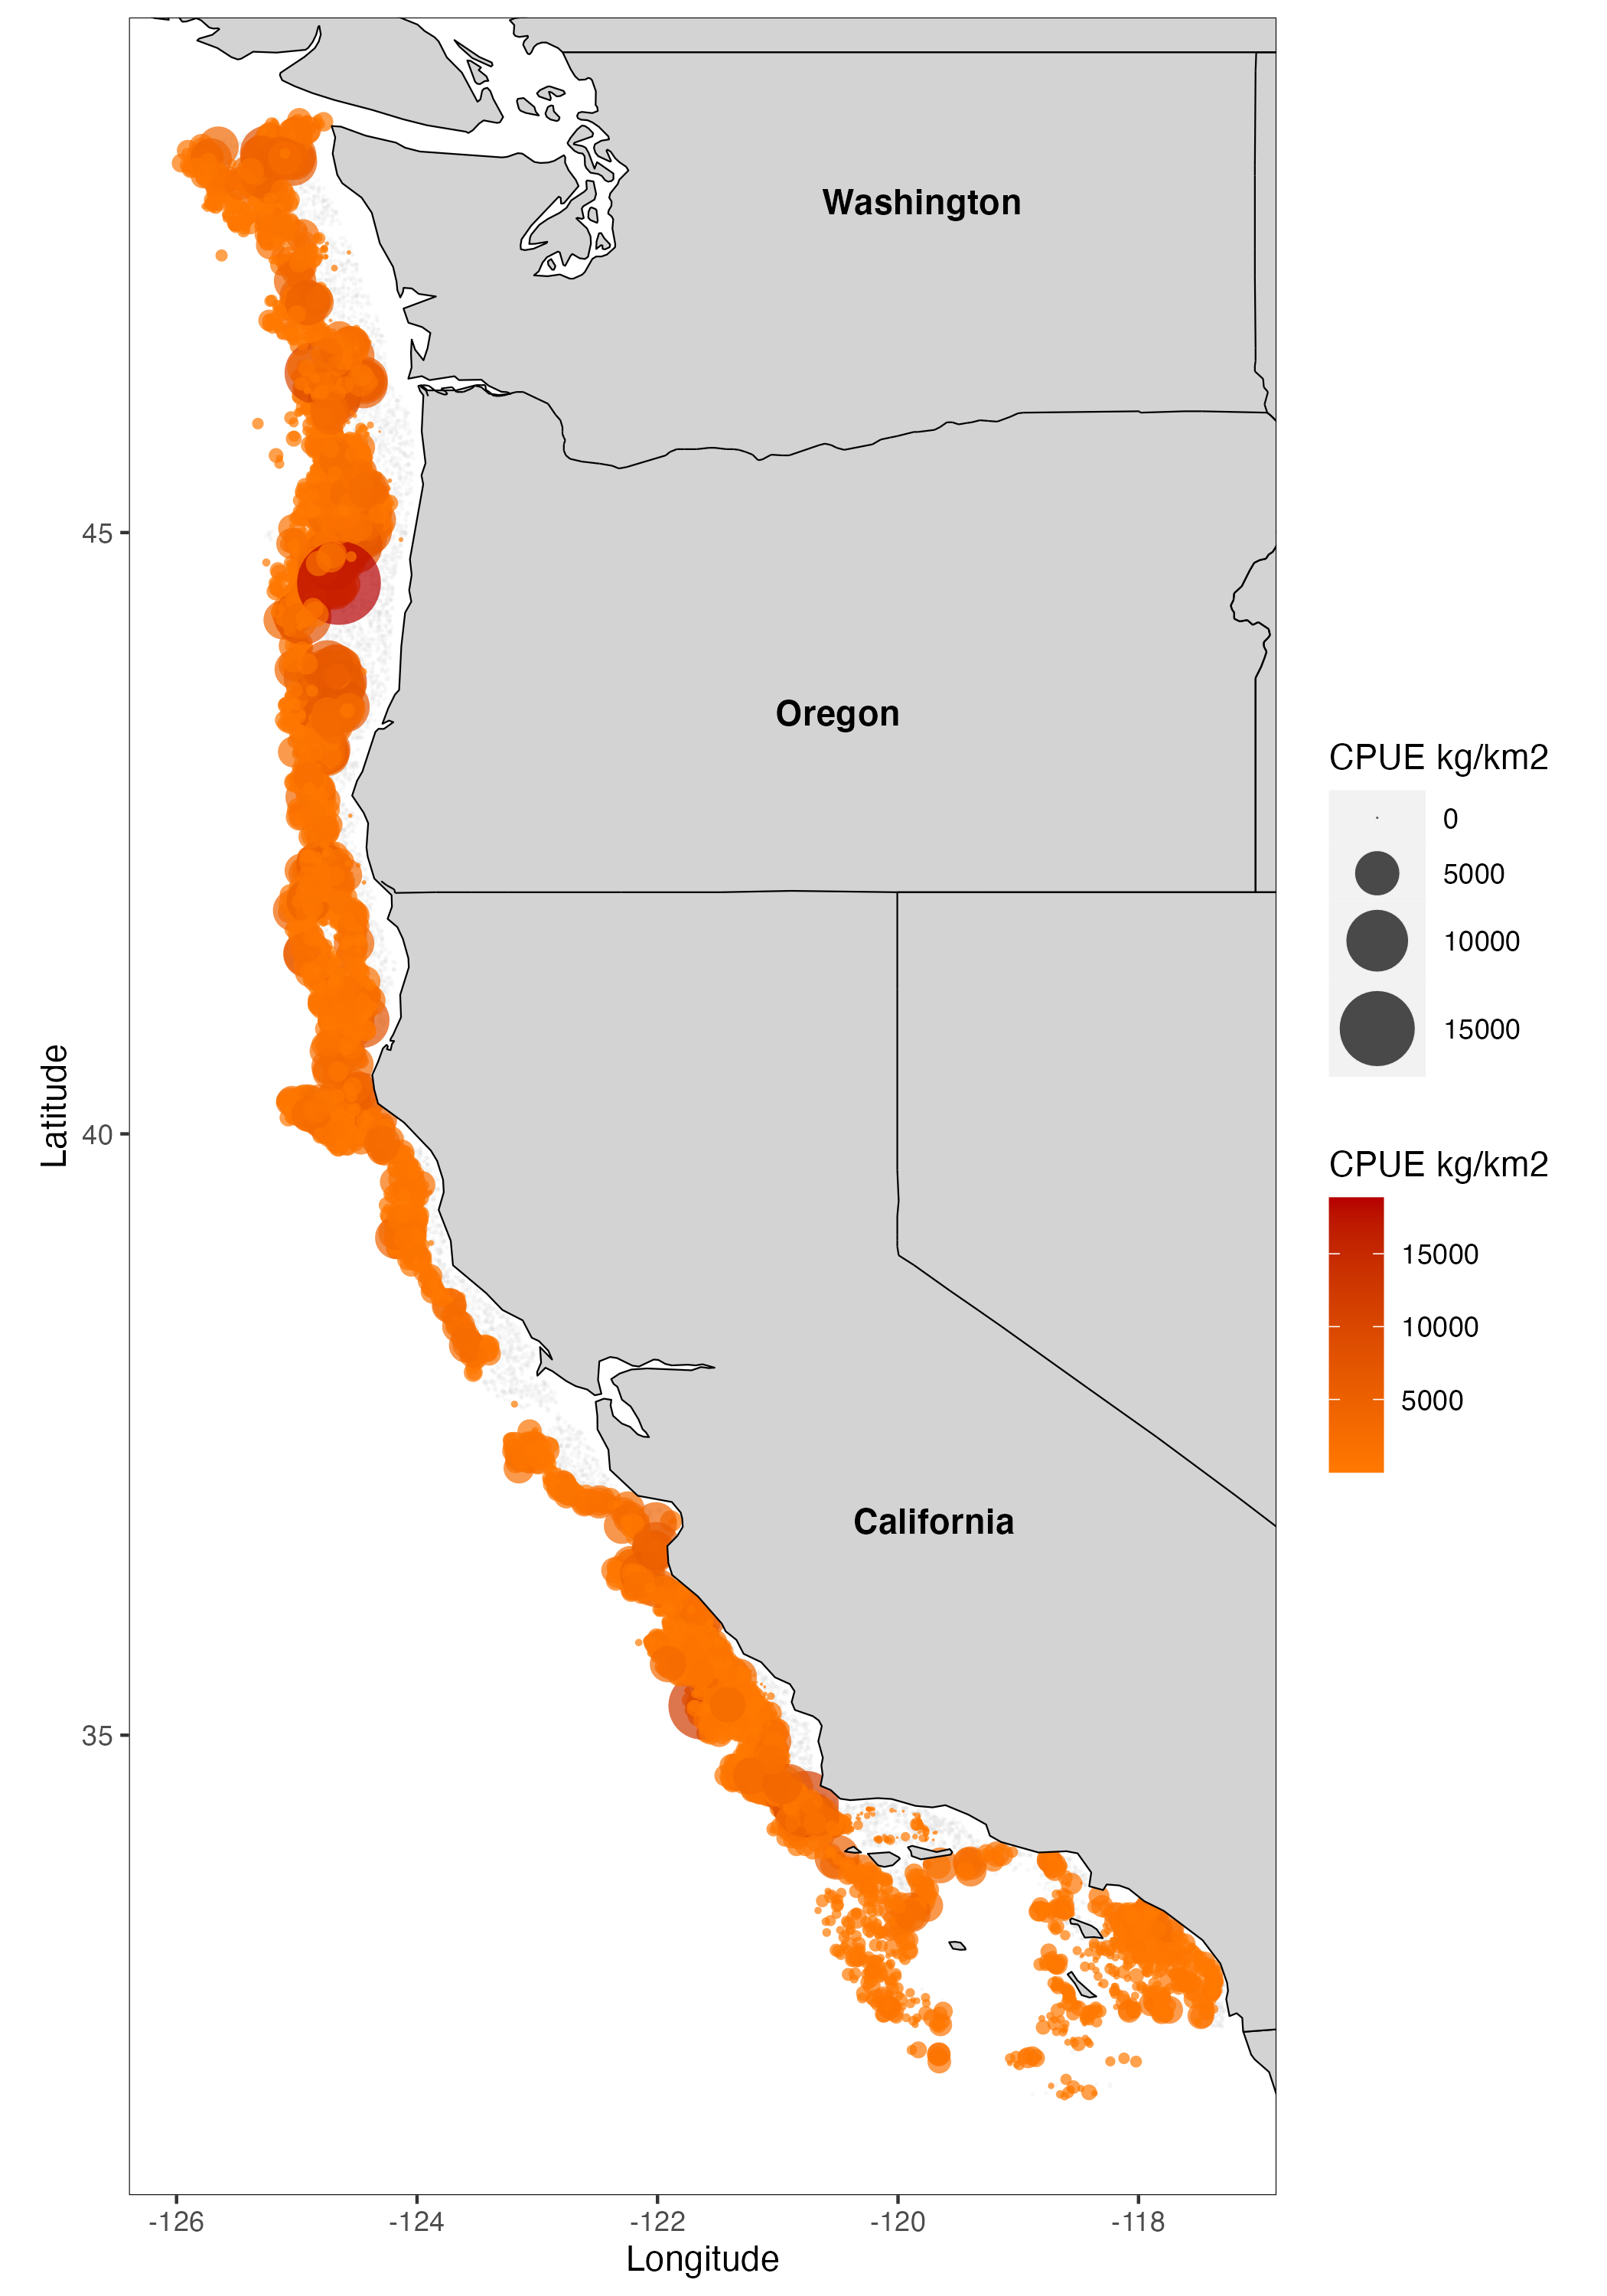
\includegraphics[width=1\textwidth,height=1\textheight]{/Users/jzahner/Desktop/Projects/shortspine_thornyhead_2023/doc/FinalFigs/Intro/stock-map.png}
\caption{Biomass of shortspine thornyhead found in the NWFSC West Coast Groundfish Bottom Trawl Survey annual survey (2003-2022) coastwide.\label{fig:stock-map}}
\end{figure}

\begin{figure}
\centering
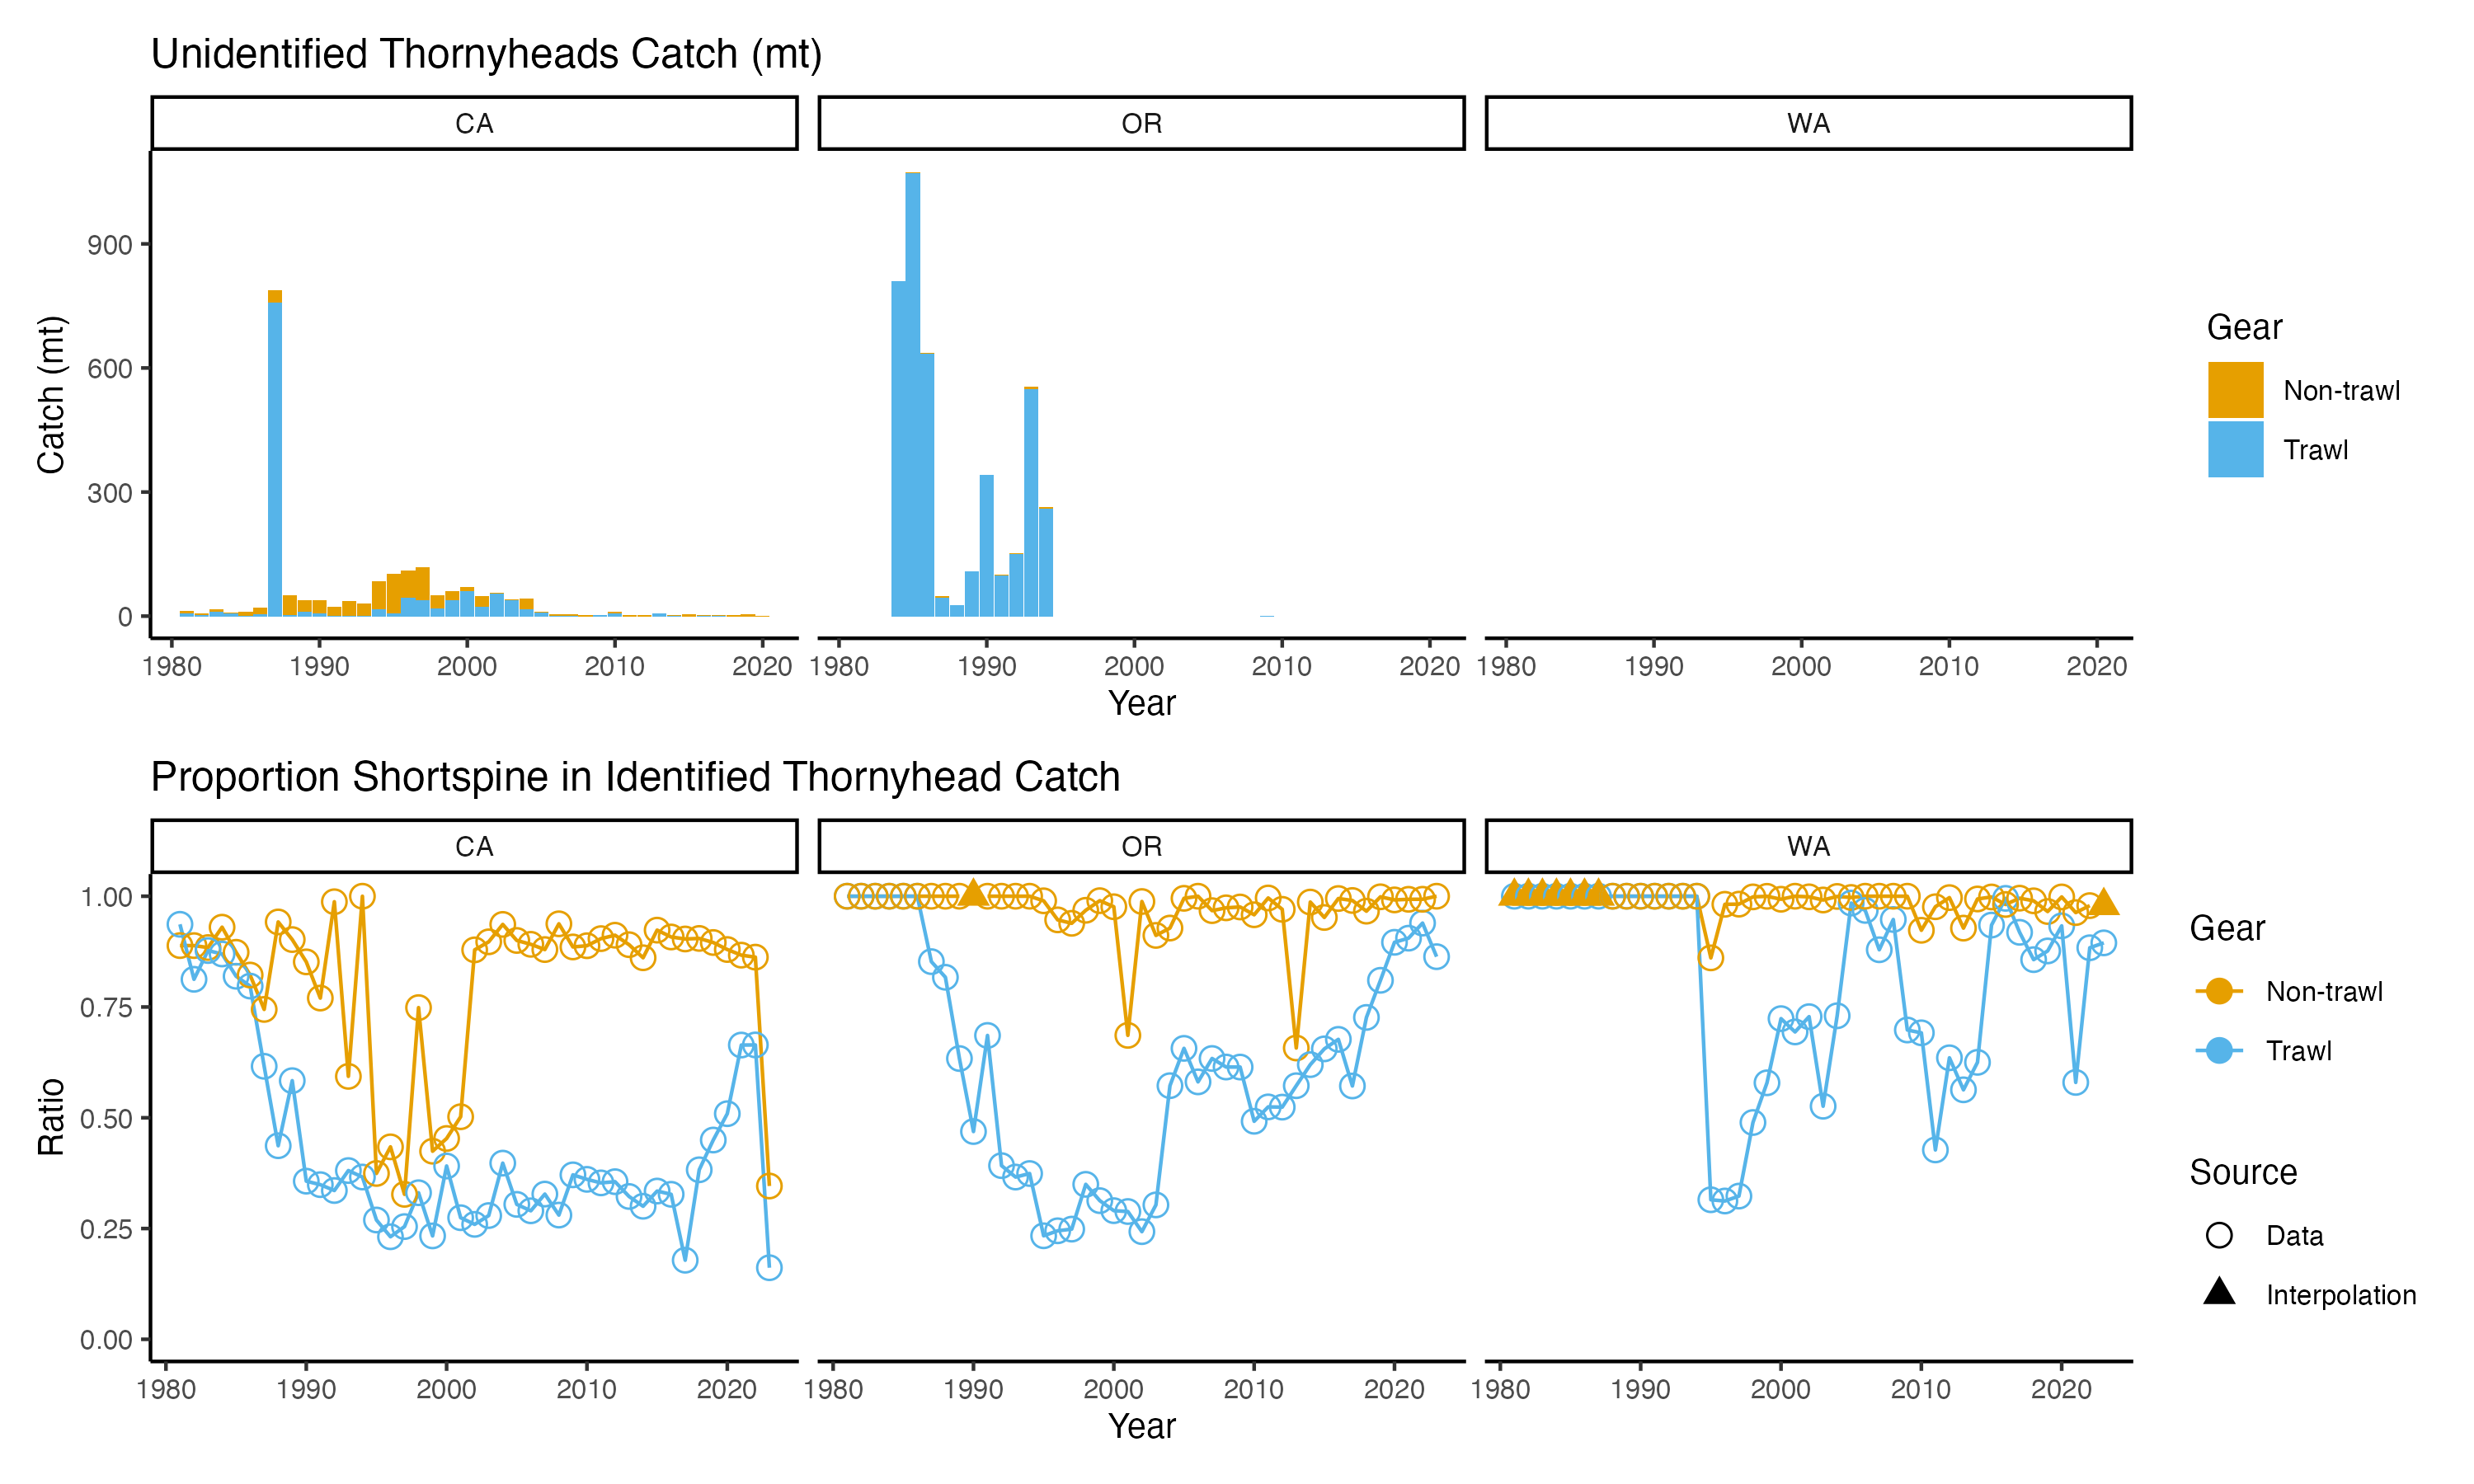
\includegraphics[width=1\textwidth,height=1\textheight]{/Users/jzahner/Desktop/Projects/shortspine_thornyhead_2023/doc/FinalFigs/Intro/thornyhead-ratio.png}
\caption{Unidentified thornyhead catches (mt) and the proportion identified as shortspines, calculated as the ratio of shortspine thornyhead catches to combined longspine and shortspine catches.\label{fig:thornyhead-ratio}}
\end{figure}

\newpage

\clearpage

\begin{figure}
\centering
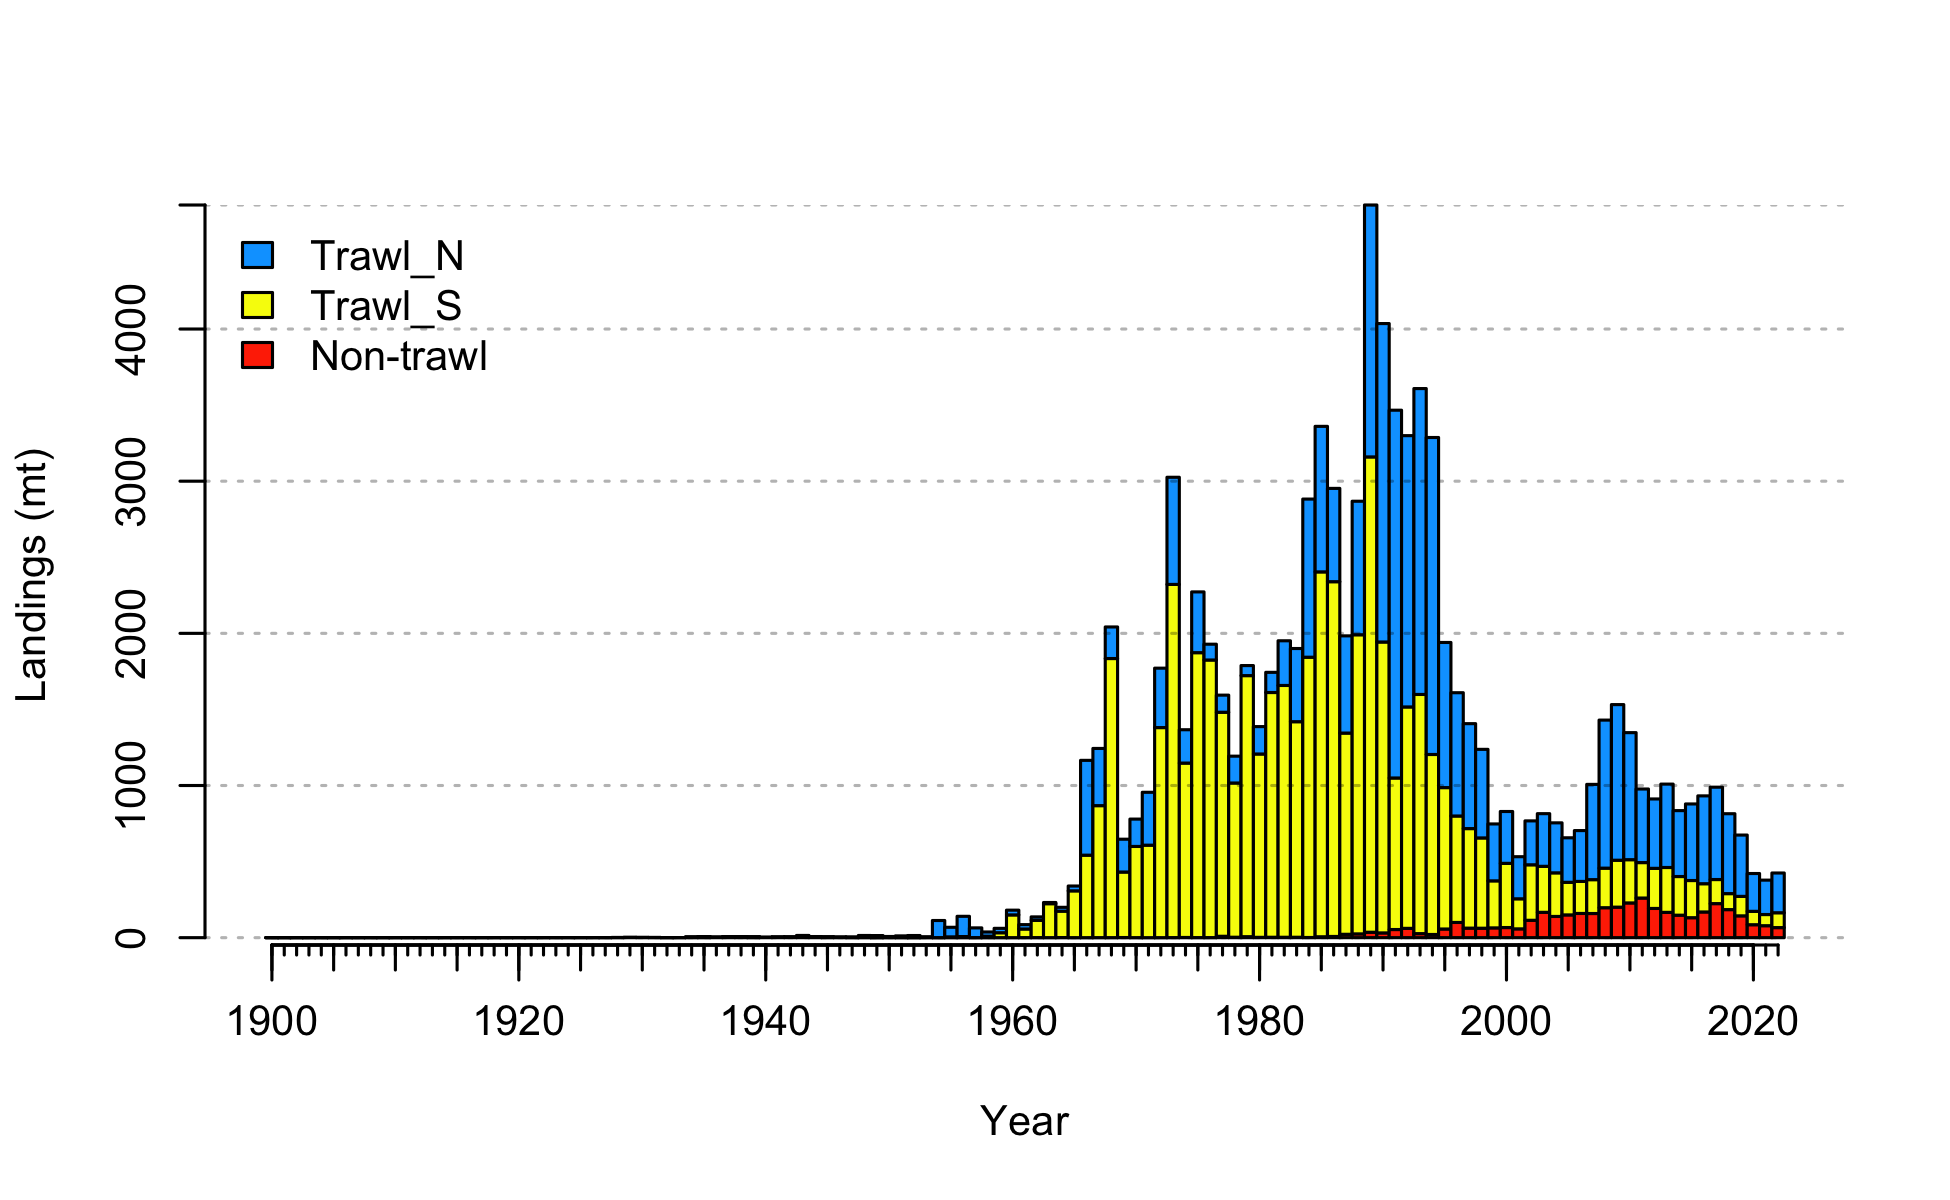
\includegraphics[width=1\textwidth,height=1\textheight]{/Users/jzahner/Desktop/Projects/shortspine_thornyhead_2023/doc/FinalFigs/Base/catch2 landings stacked.png}
\caption{Estimated landing history for shortspine thornyhead.\label{fig:catch_hist}}
\end{figure}

\newpage

\begin{figure}
\centering
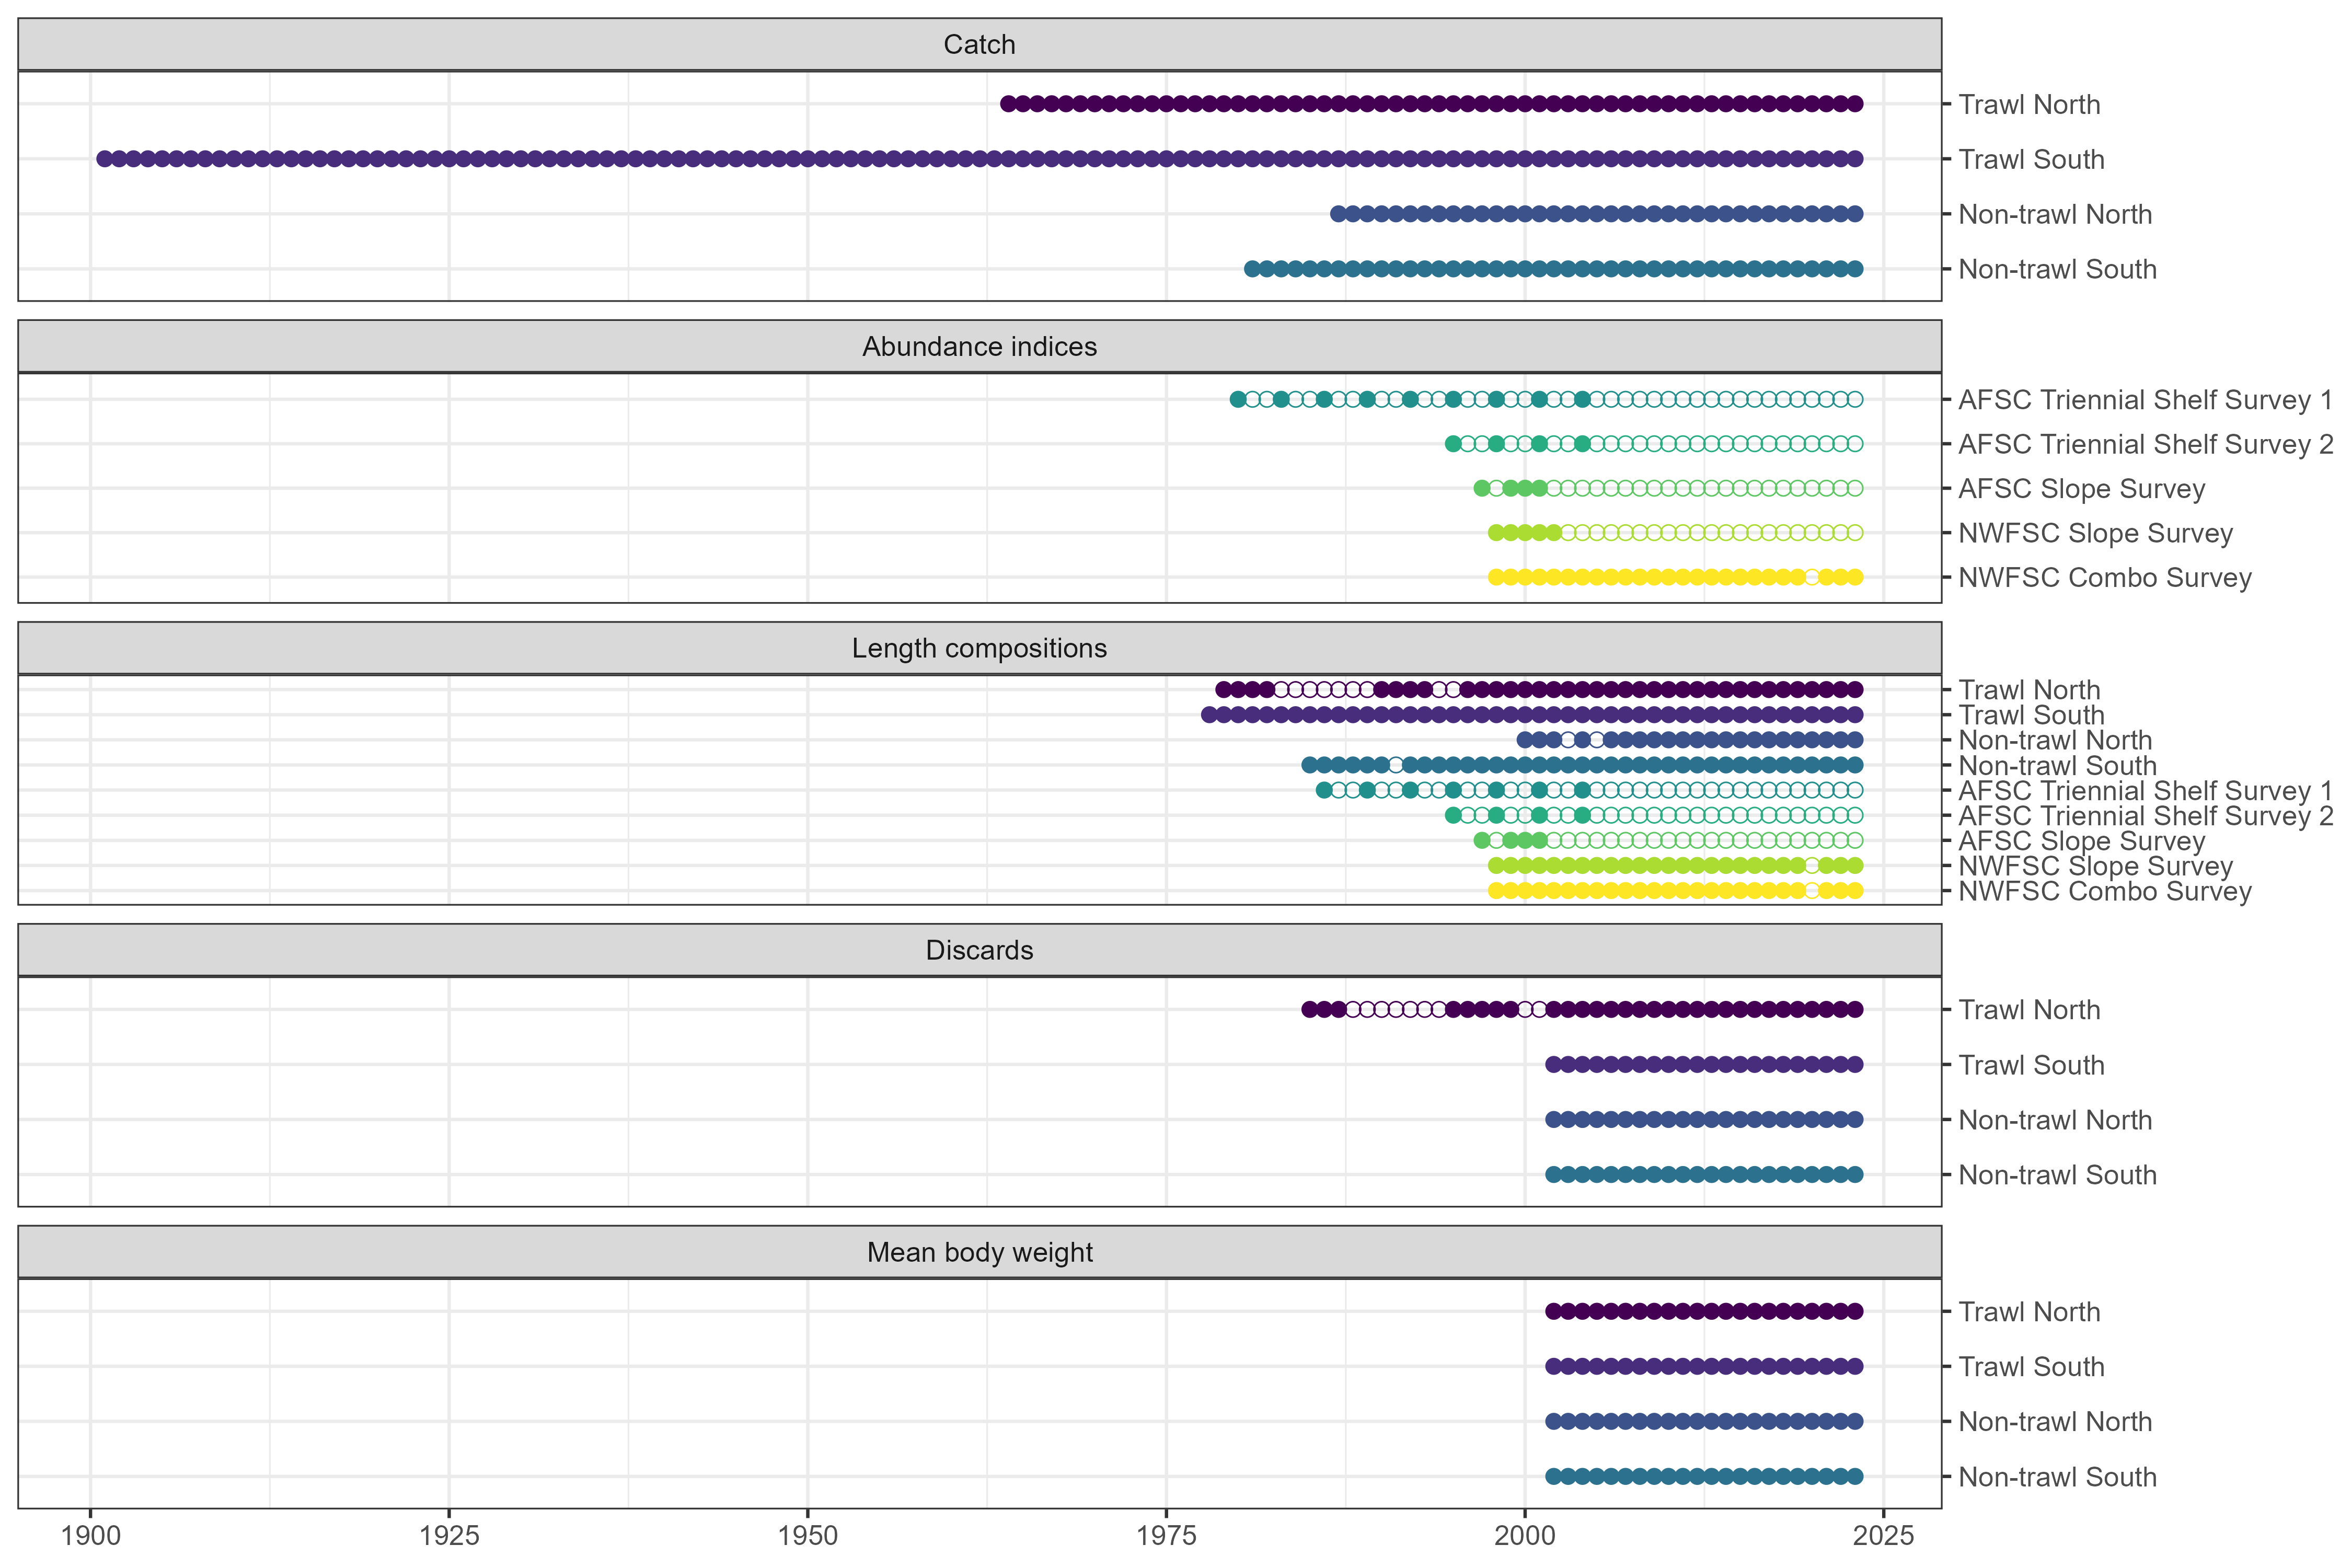
\includegraphics[width=1\textwidth,height=1\textheight]{/Users/jzahner/Desktop/Projects/shortspine_thornyhead_2023/doc/FinalFigs/Data/assessment_data_timeseries.png}
\caption{Summary of data sources used in the base model.\label{fig:assessment_data_timeseries}}
\end{figure}

\begin{figure}
\centering
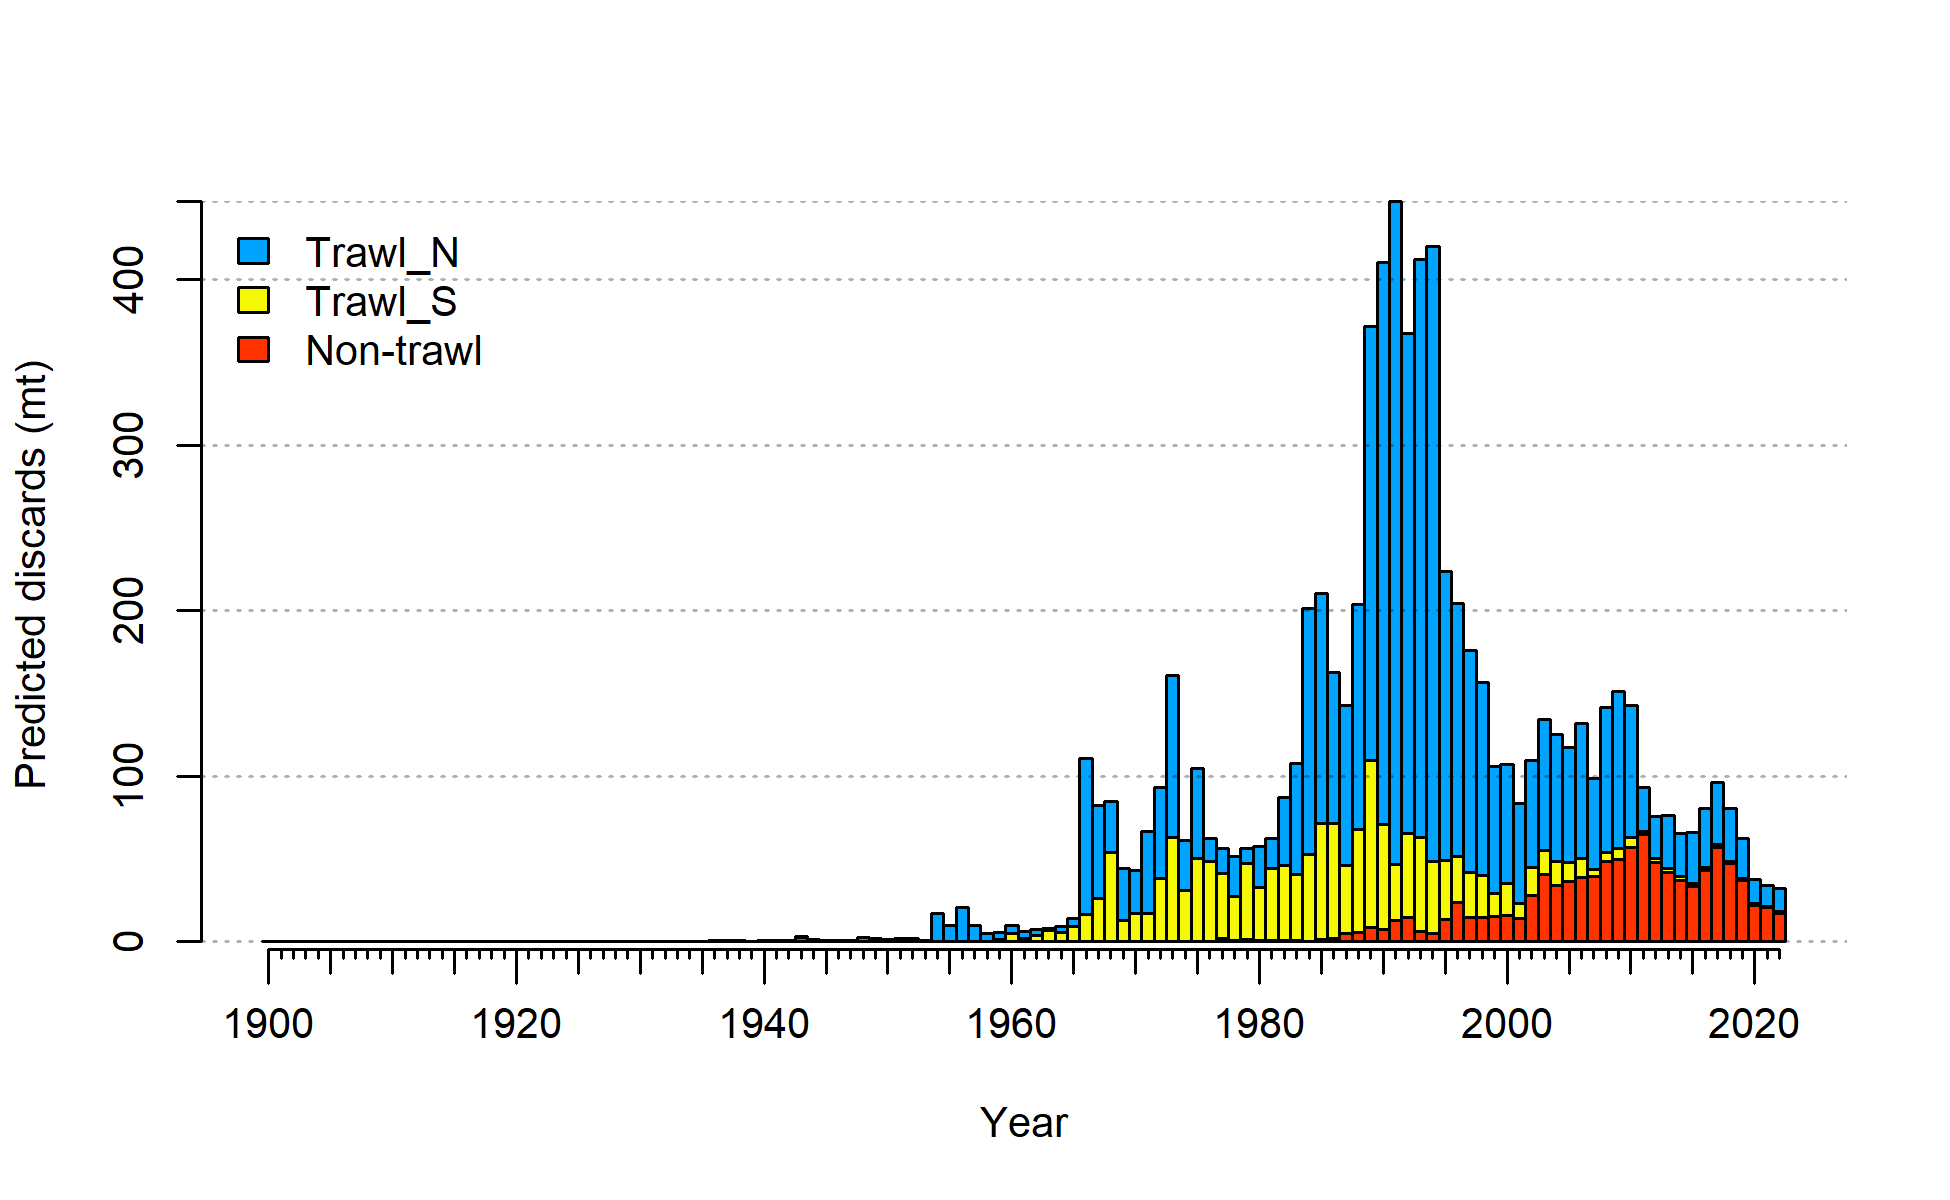
\includegraphics[width=1\textwidth,height=1\textheight]{/Users/jzahner/Desktop/Projects/shortspine_thornyhead_2023/doc/FinalFigs/Base/catch7 discards stacked plot (depends on multiple fleets).png}
\caption{Predicted discards based estimated retention and selectivity for each fleet.\label{fig:disc_hist}}
\end{figure}

\begin{figure}
\centering
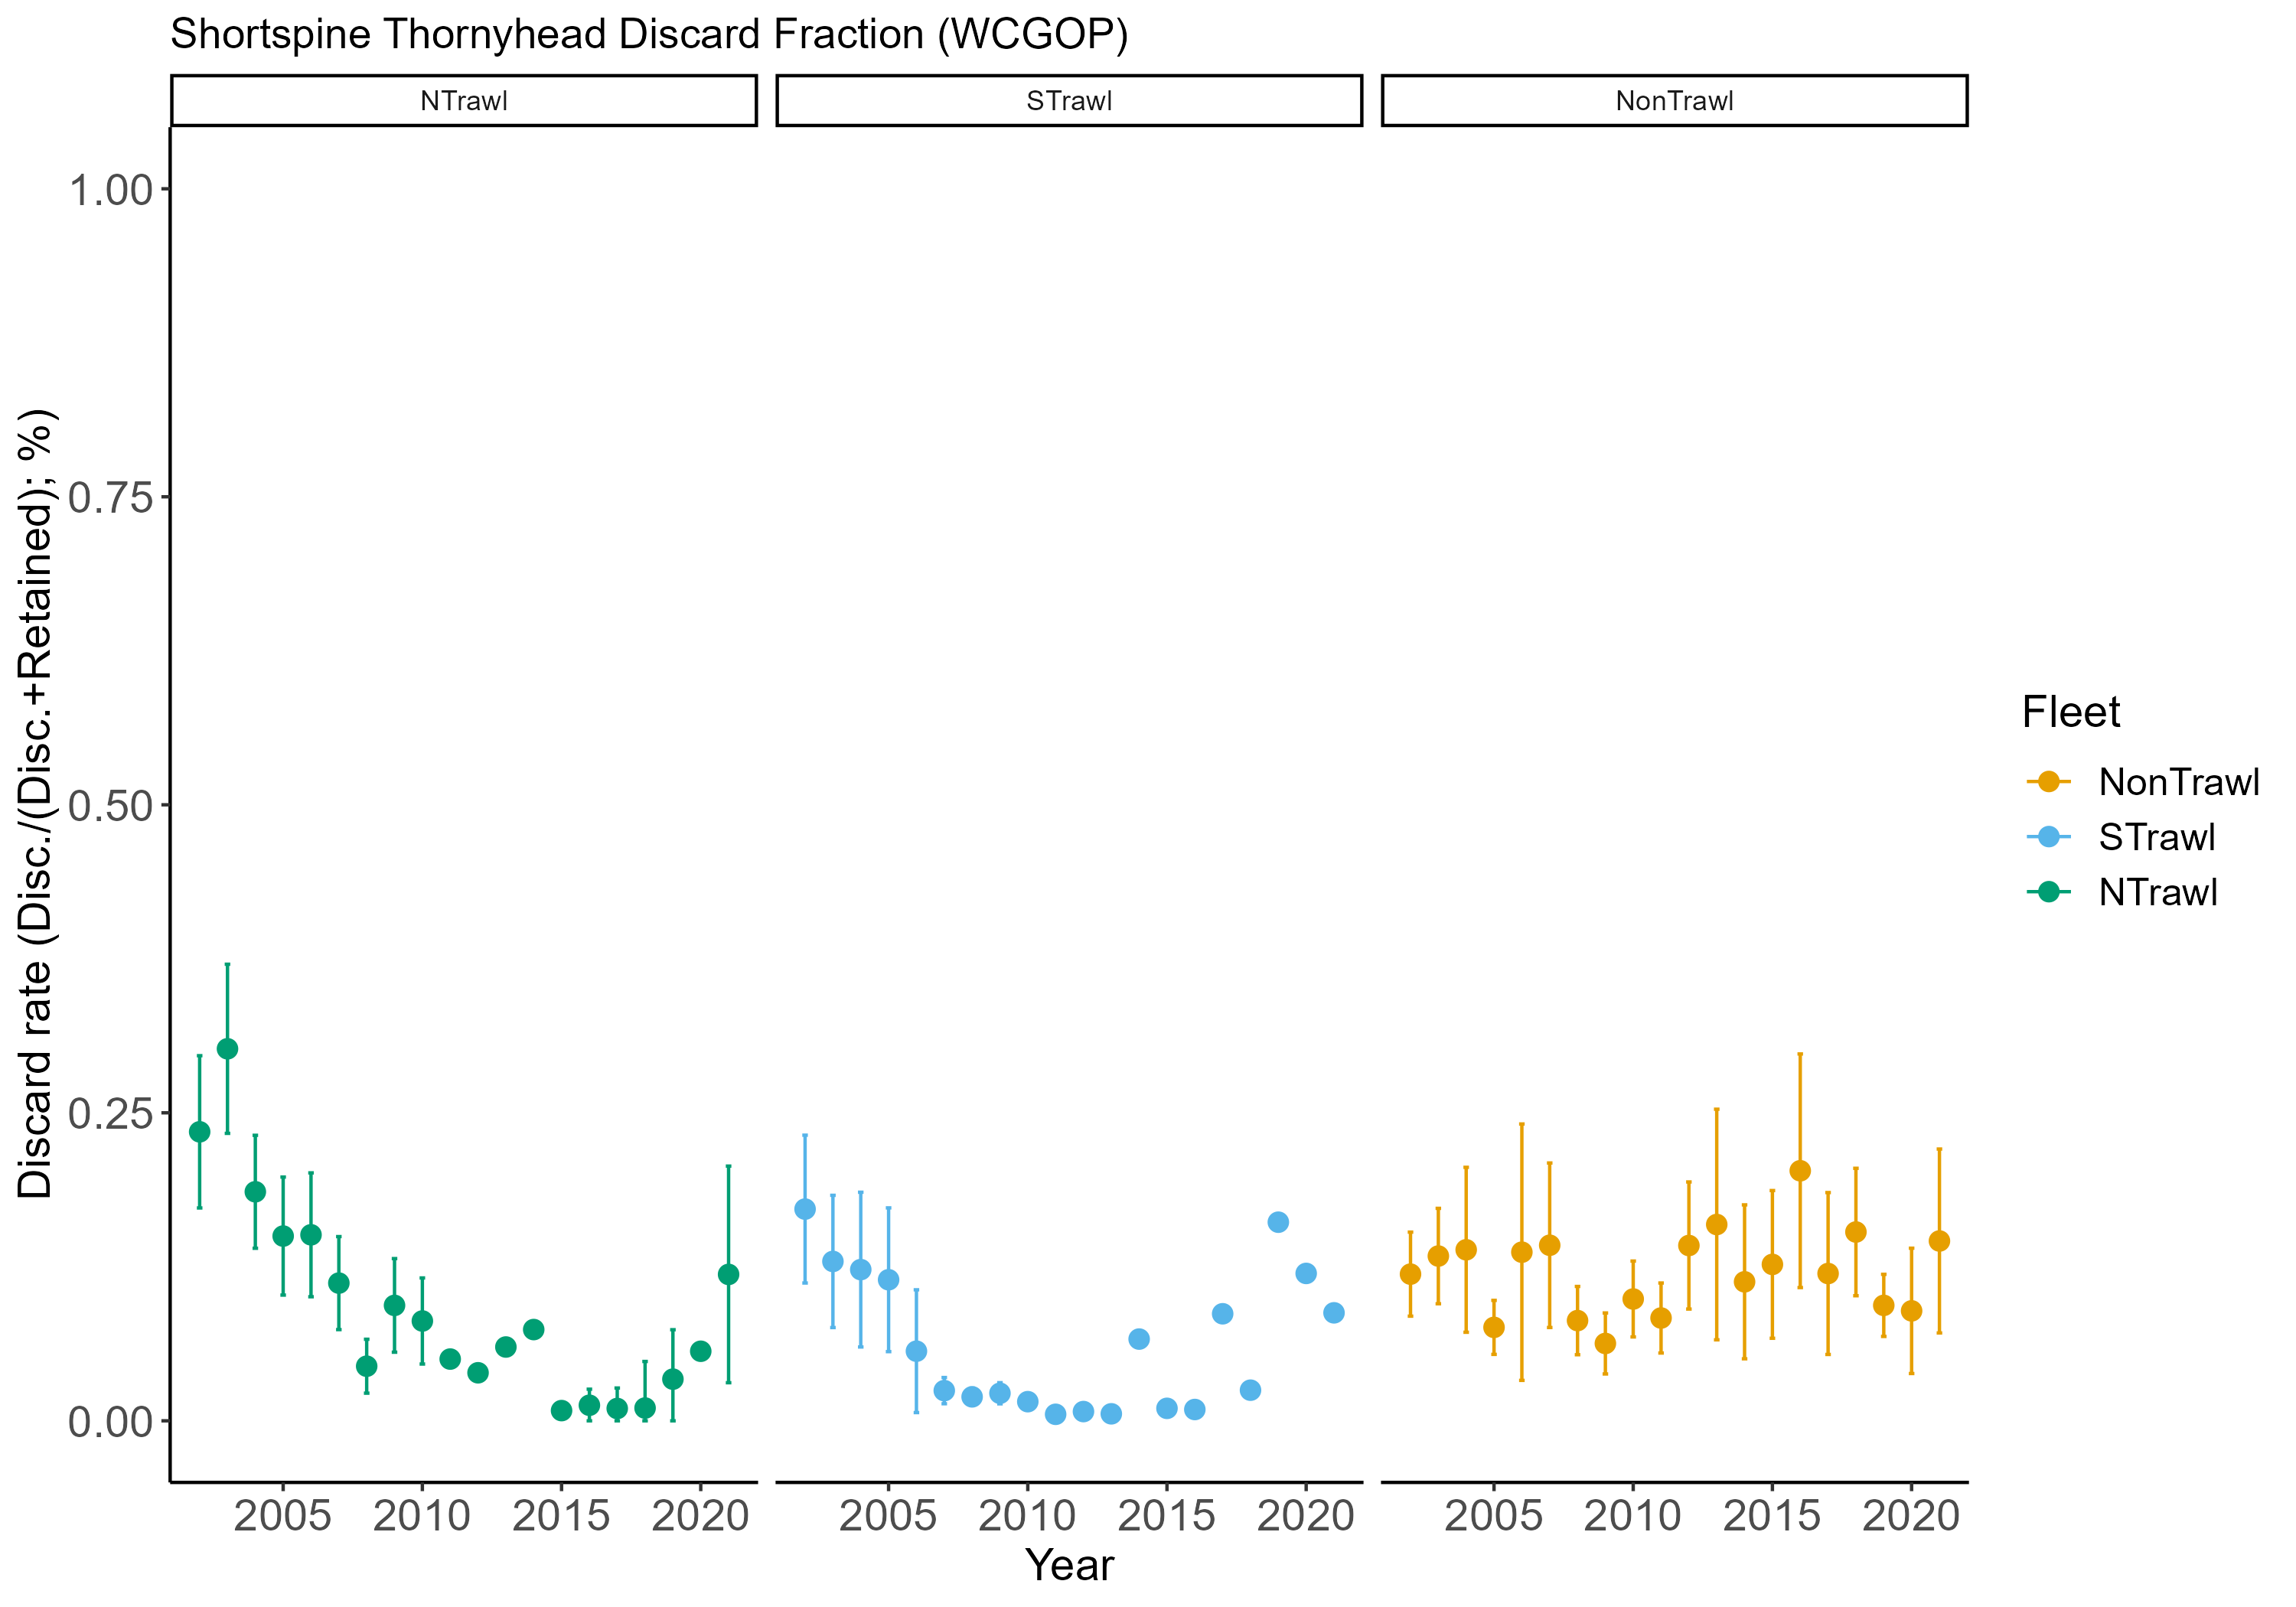
\includegraphics[width=1\textwidth,height=1\textheight]{/Users/jzahner/Desktop/Projects/shortspine_thornyhead_2023/doc/FinalFigs/Data/SST_WCGOP_GEMM_discard_rates_3fleet.png}
\caption{Discard rates from the WCGOP data set with catch share and non-catch share considerations from the GEMM dataset.\label{fig:disc_rates_WCGOP}}
\end{figure}

\newpage

\begin{figure}
\centering
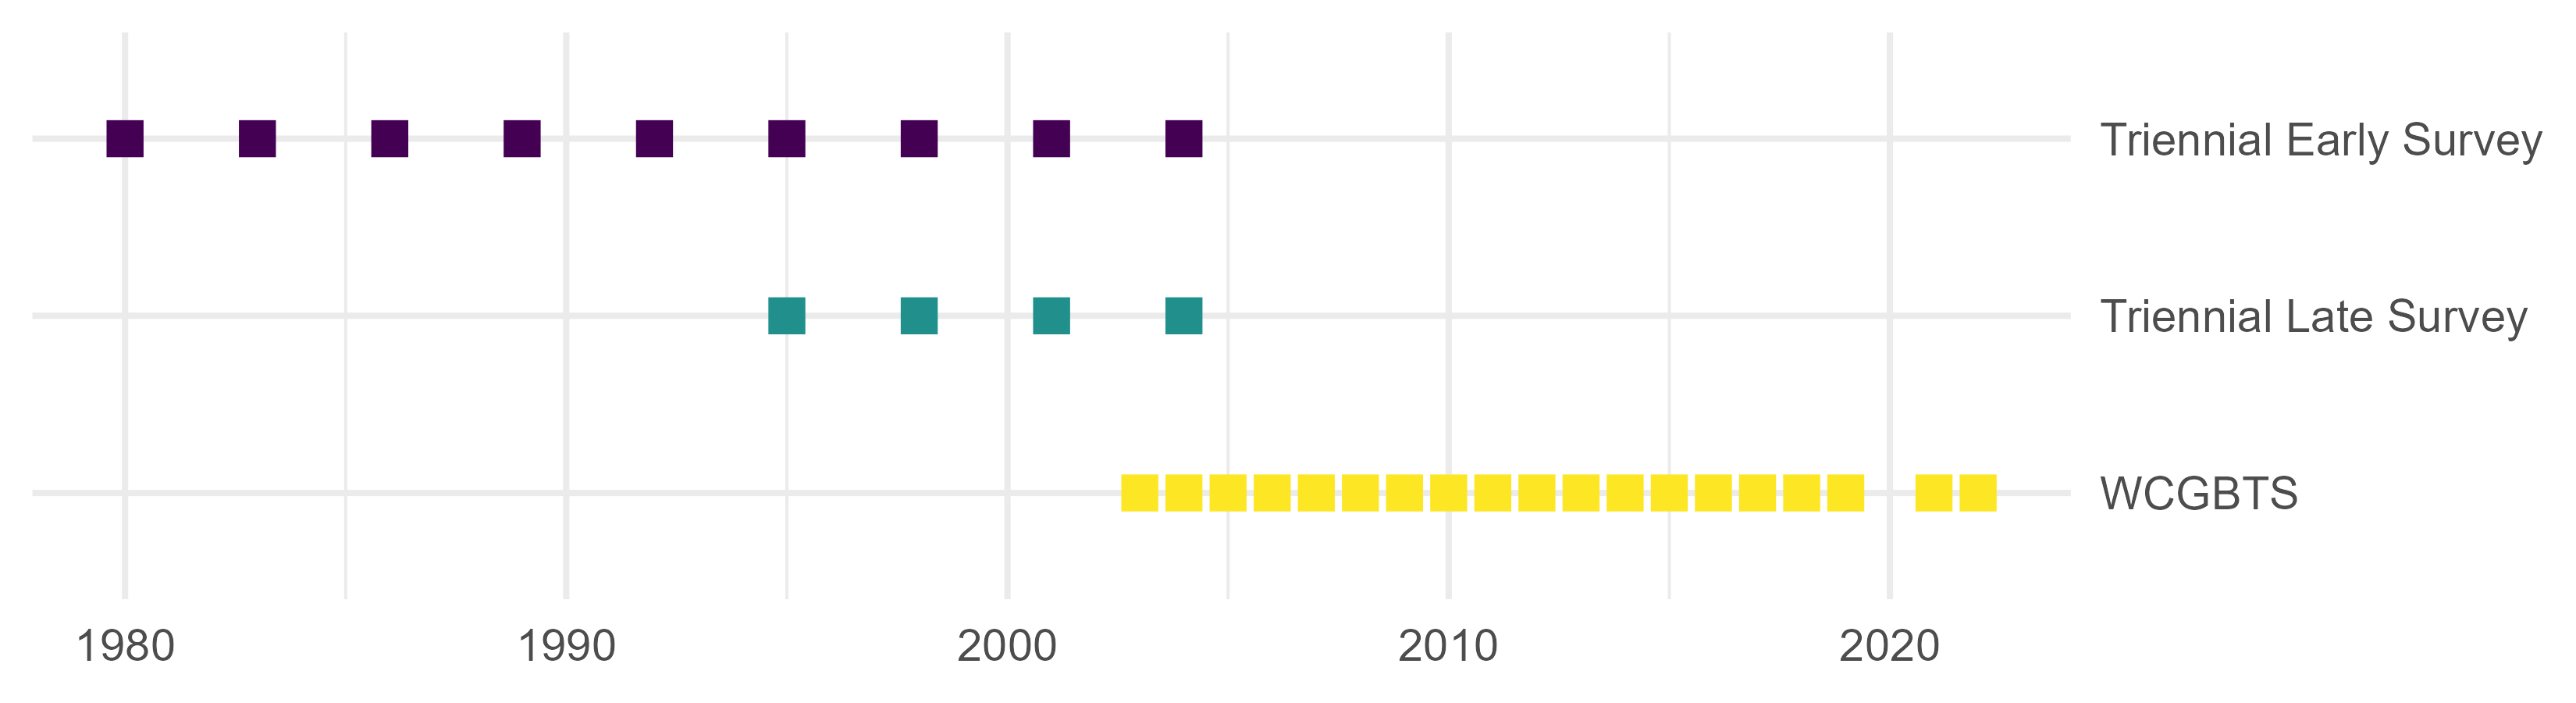
\includegraphics[width=1\textwidth,height=1\textheight]{/Users/jzahner/Desktop/Projects/shortspine_thornyhead_2023/doc/FinalFigs/Data/survey_data_timeseries.png}
\caption{Summary of survey data sources used in the base model.\label{fig:survey_data_timeseries}}
\end{figure}

\begin{figure}
\centering
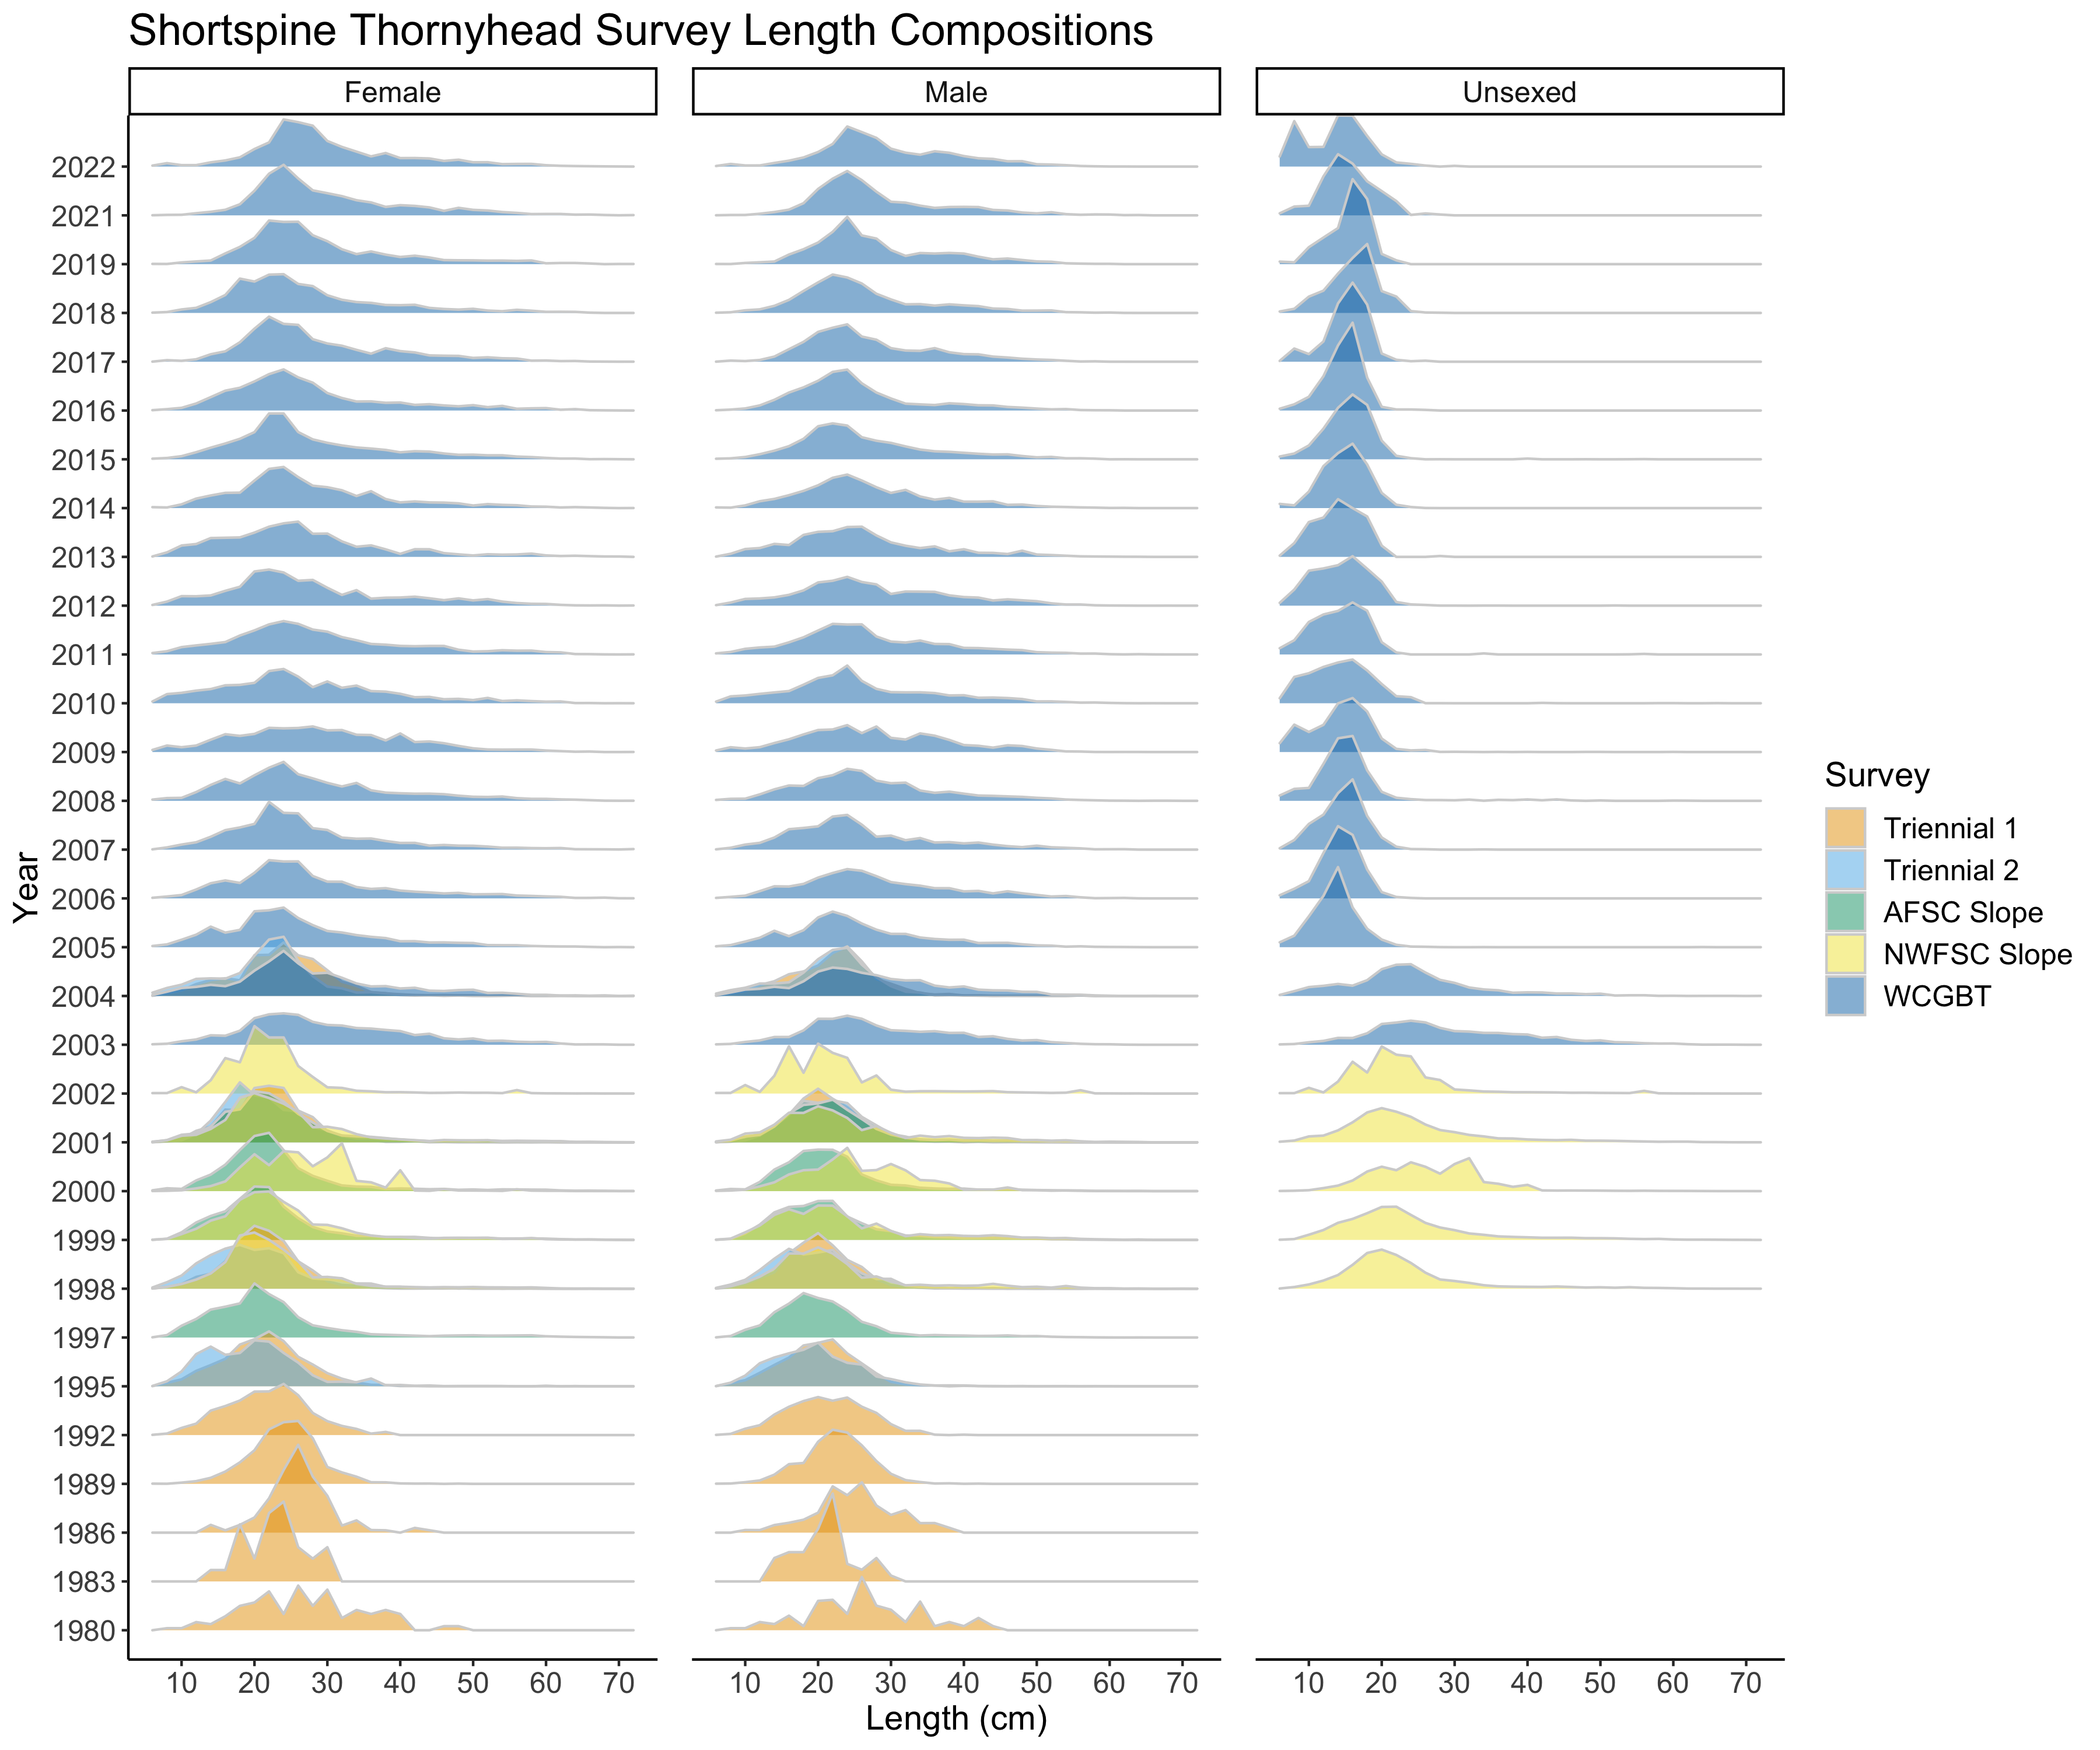
\includegraphics[width=1\textwidth,height=1\textheight]{/Users/jzahner/Desktop/Projects/shortspine_thornyhead_2023/doc/FinalFigs/Data/2023_length_compositions.png}
\caption{Survey length composition data.\label{fig:survey_comps}}
\end{figure}

\begin{figure}
\centering
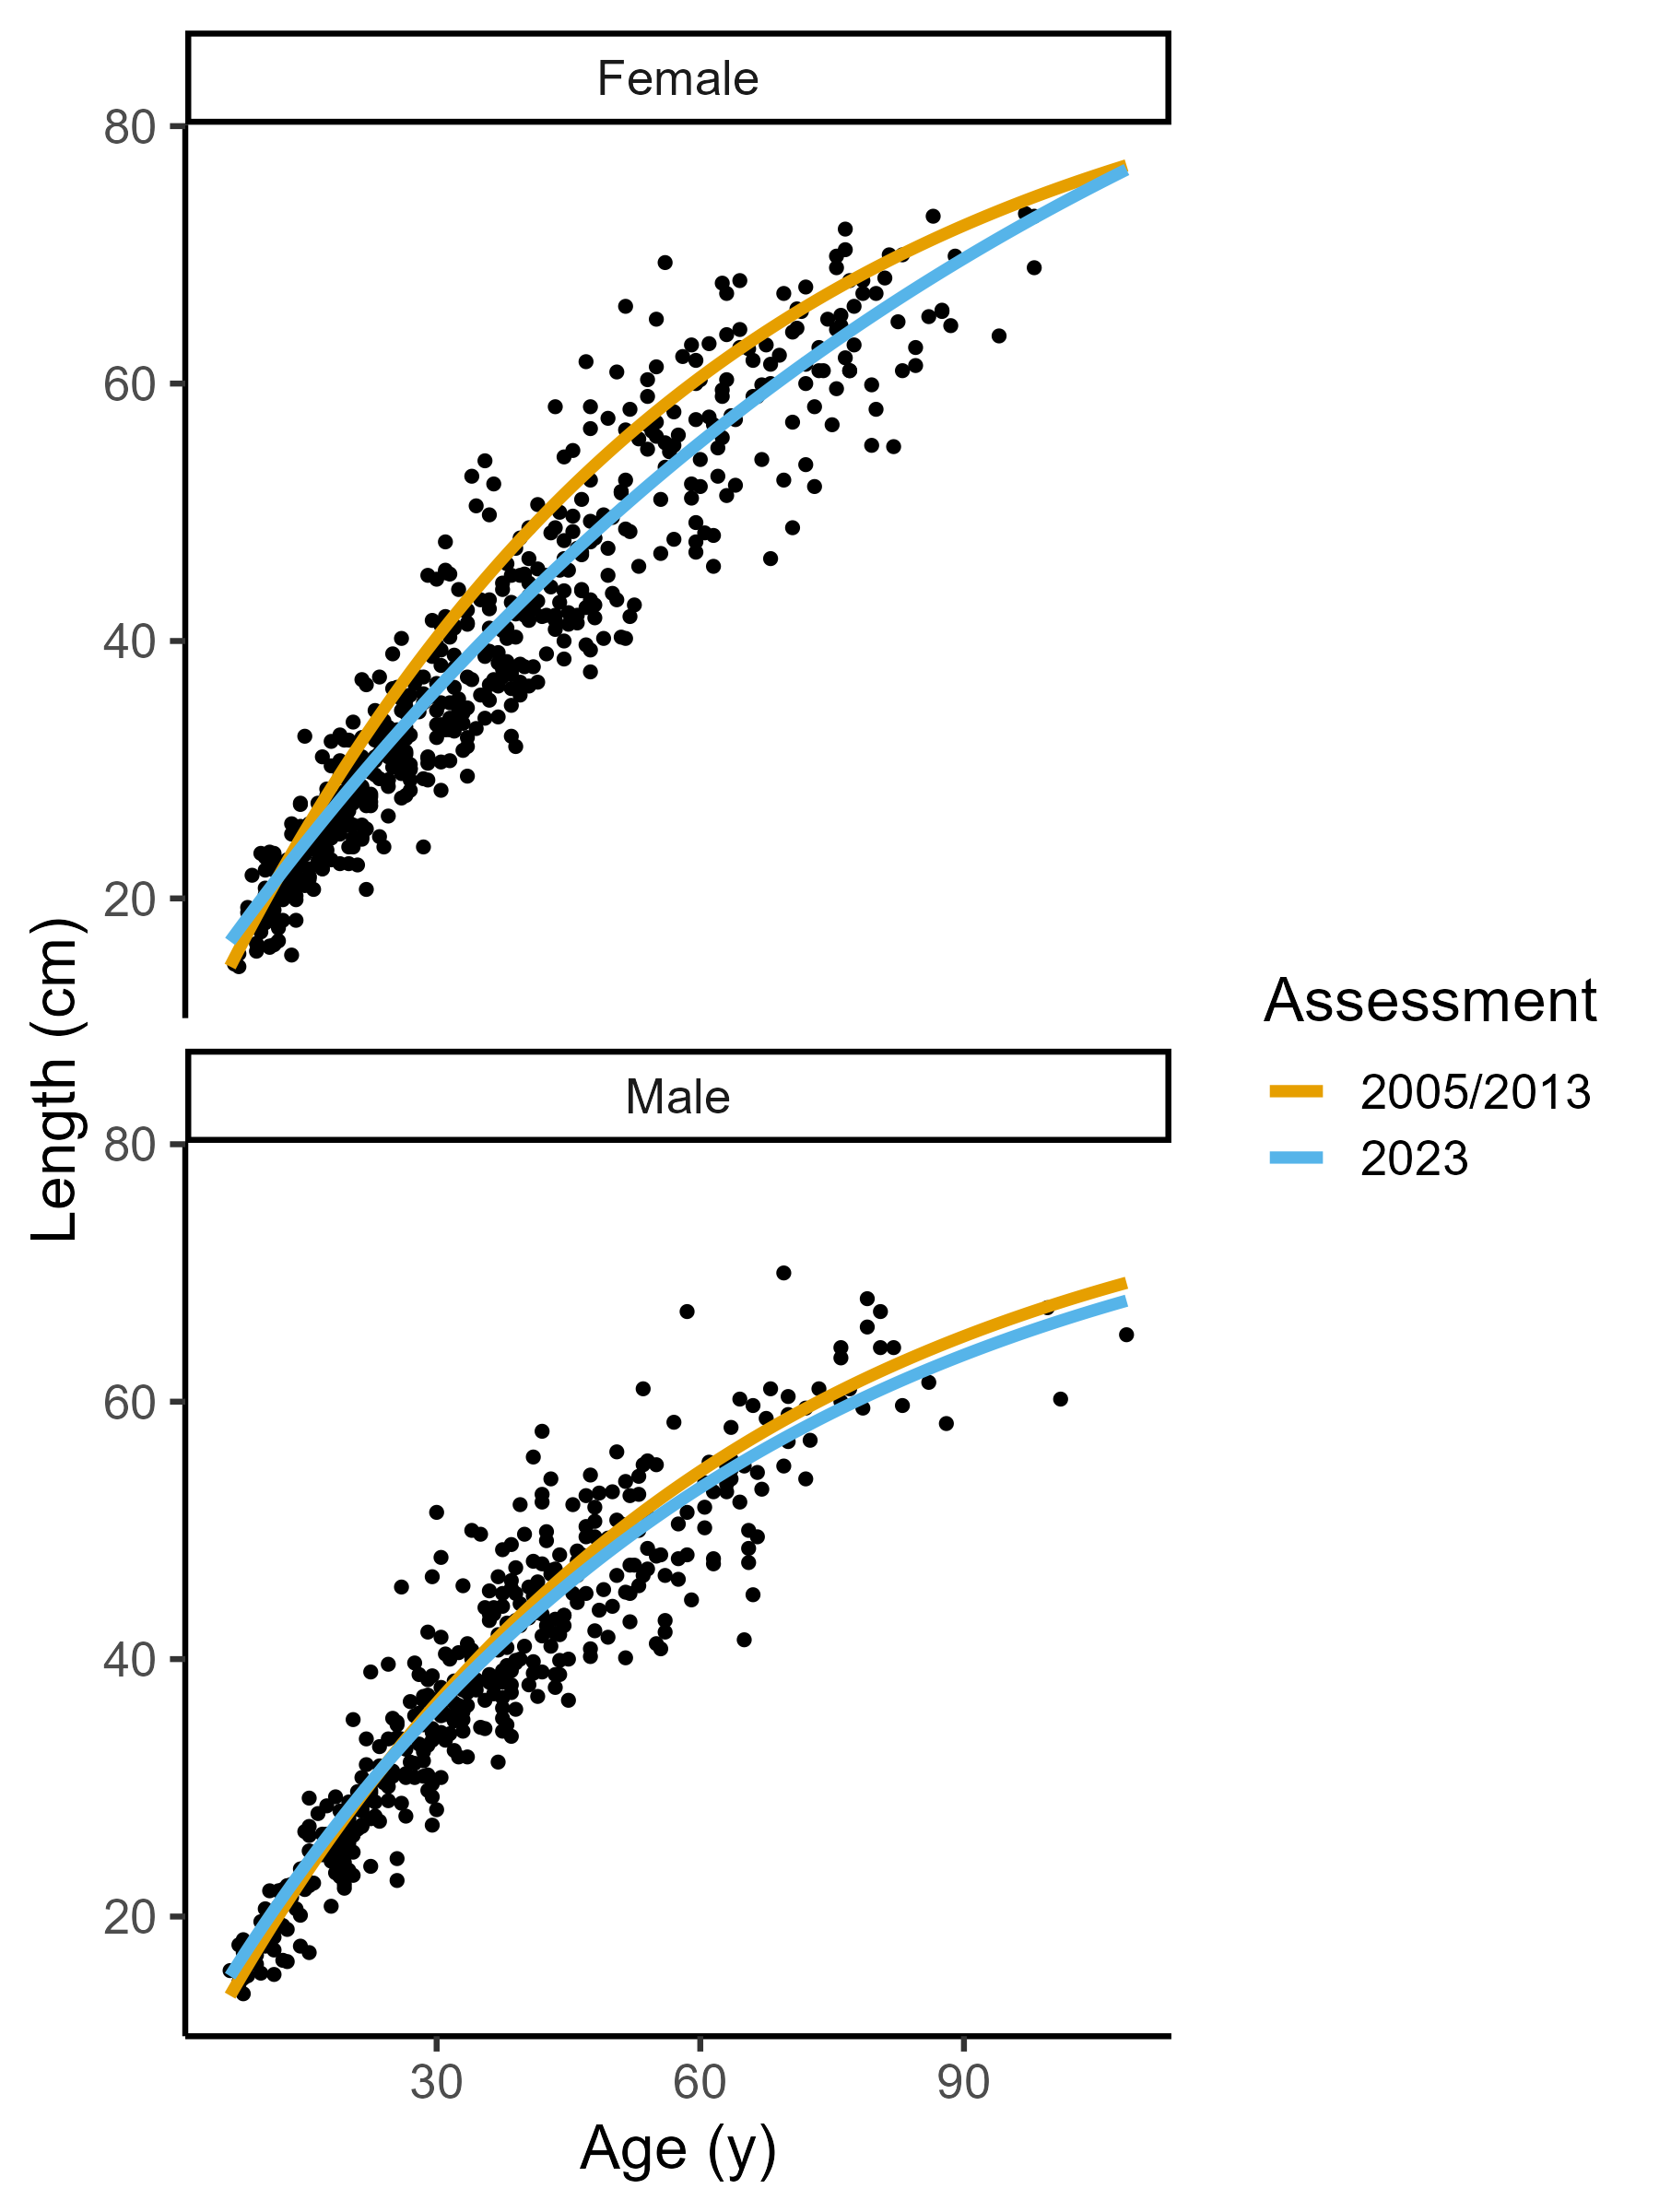
\includegraphics[width=1\textwidth,height=1\textheight]{/Users/jzahner/Desktop/Projects/shortspine_thornyhead_2023/doc/FinalFigs/Data/growth_curve_comparison_LAA1.png}
\caption{Growth curve comparison. .\label{fig:growth_LAA1}}
\end{figure}

\begin{figure}
\centering
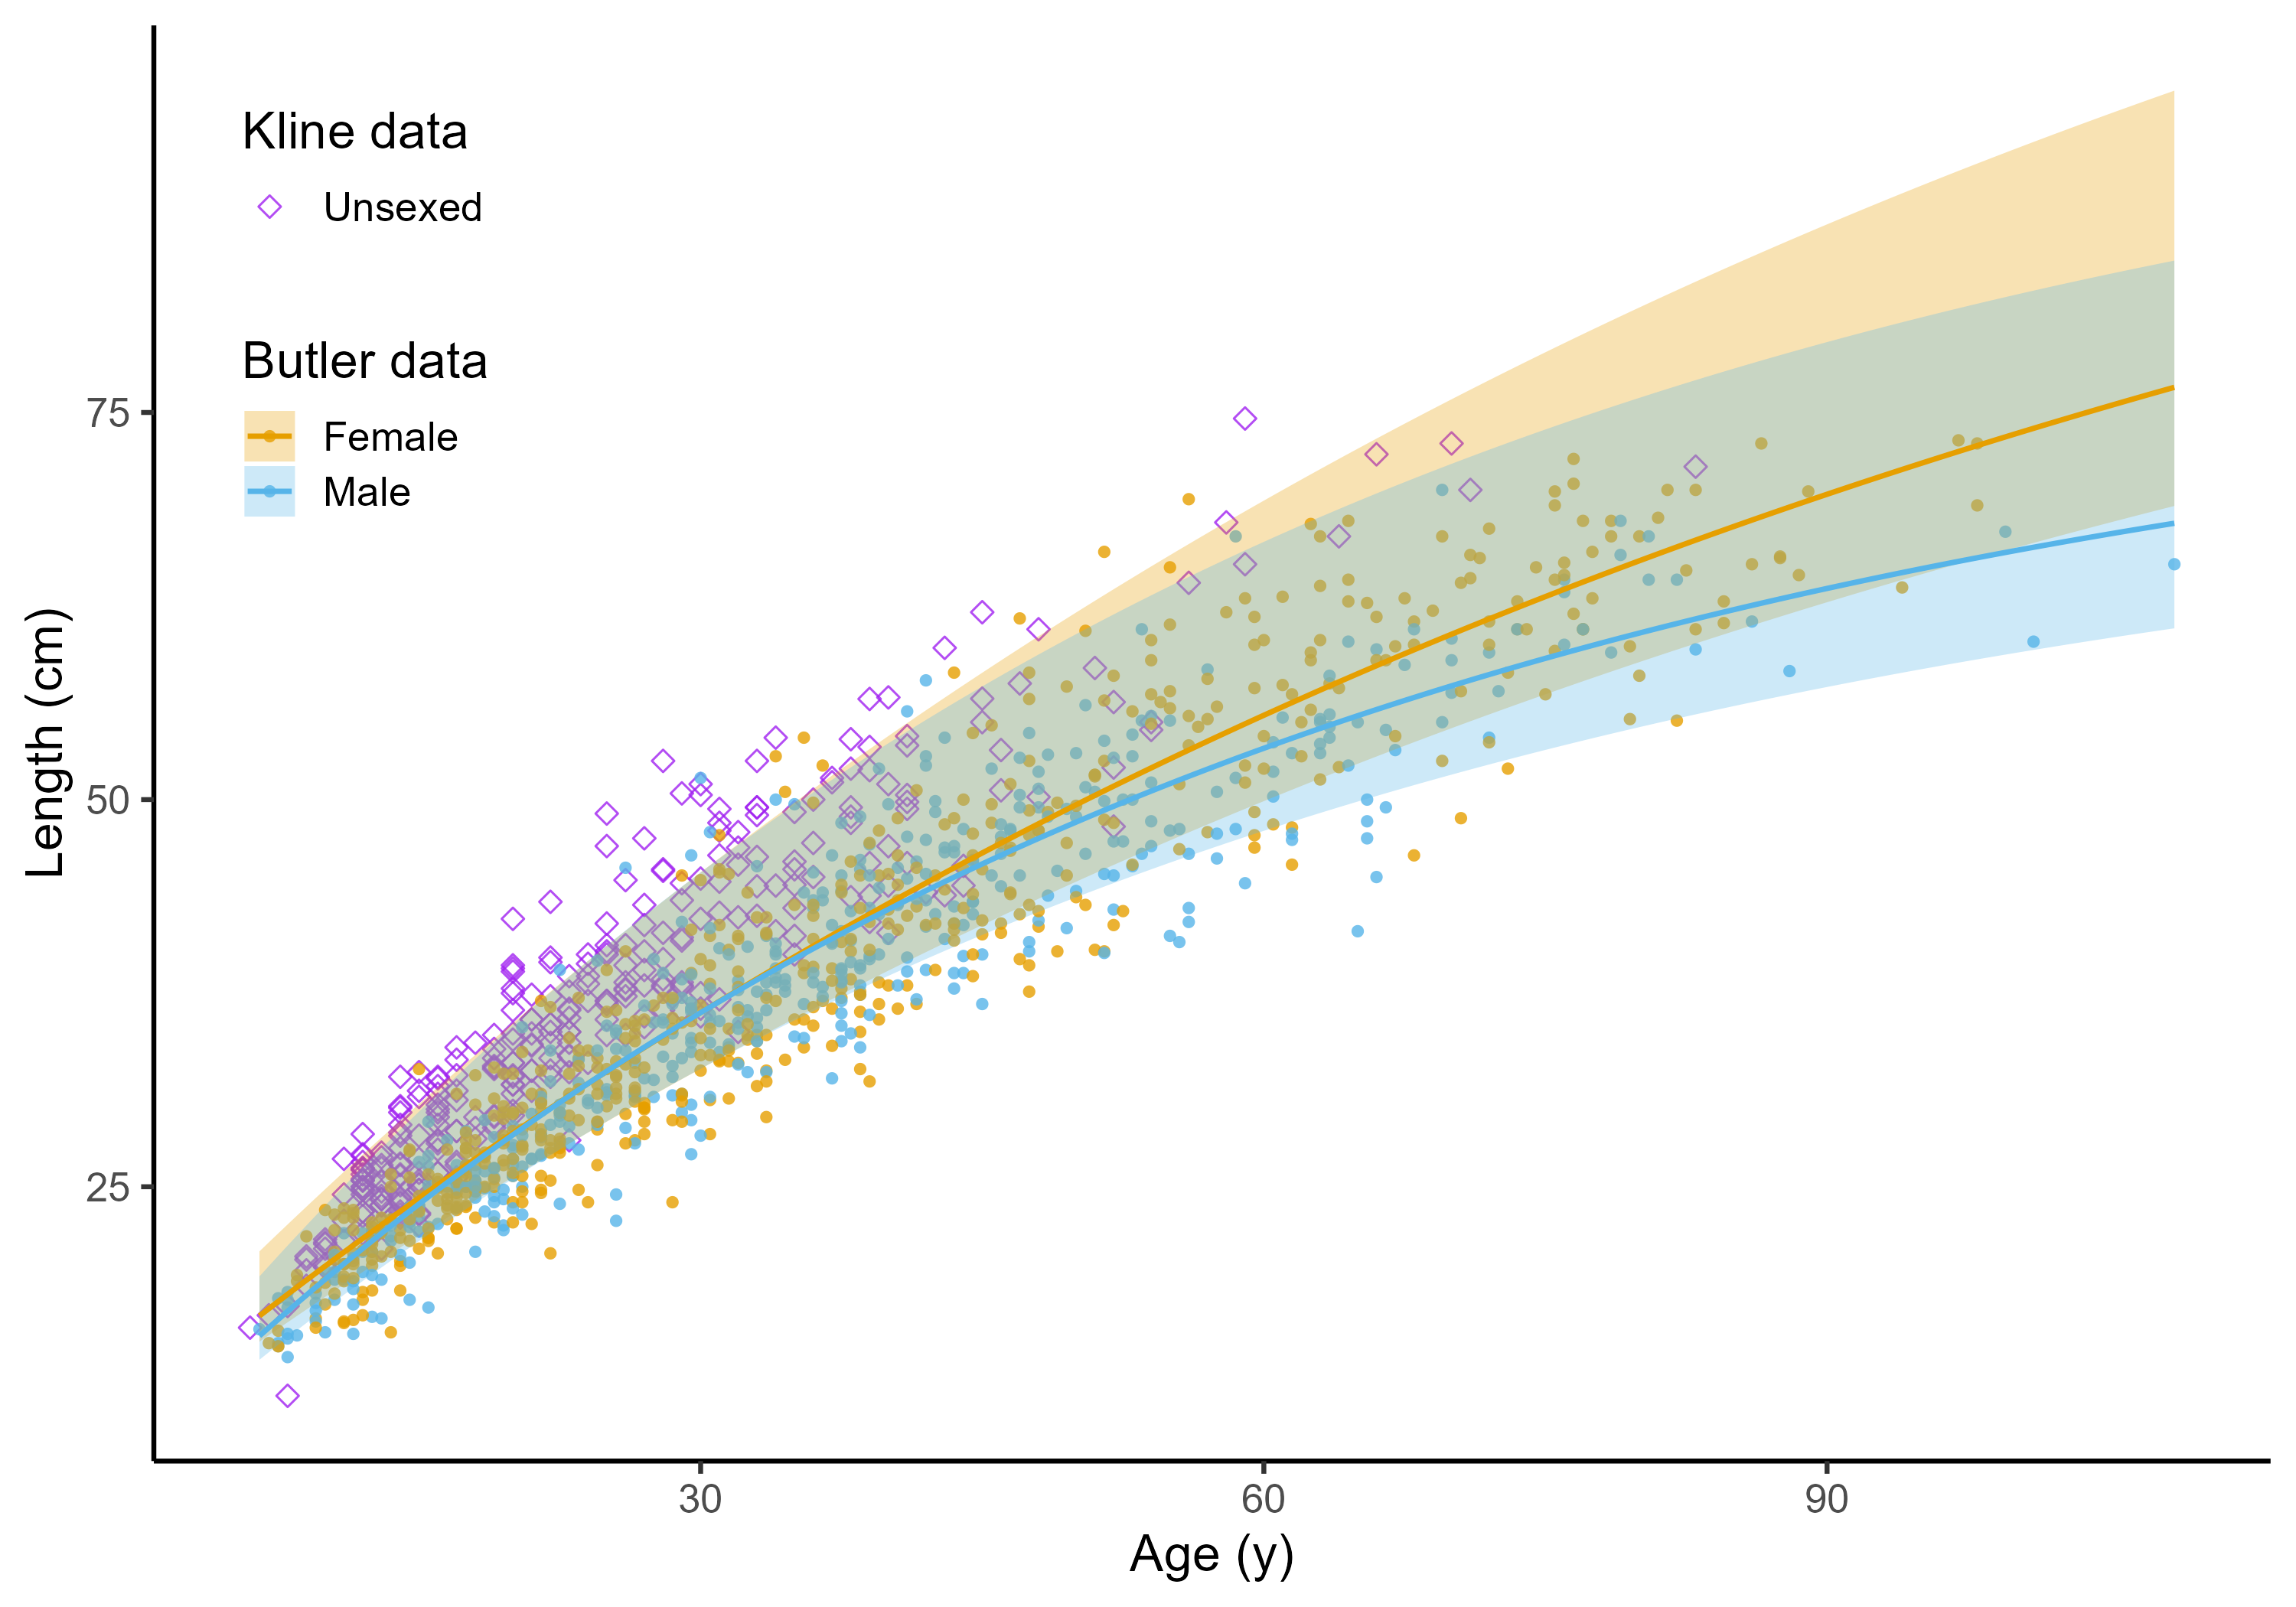
\includegraphics[width=1\textwidth,height=1\textheight]{/Users/jzahner/Desktop/Projects/shortspine_thornyhead_2023/doc/FinalFigs/Data/growth_curve_sensitivities_LAA2.png}
\caption{Growth curve sensitivities.\label{fig:growth_LAA2}}
\end{figure}

\begin{figure}
\centering
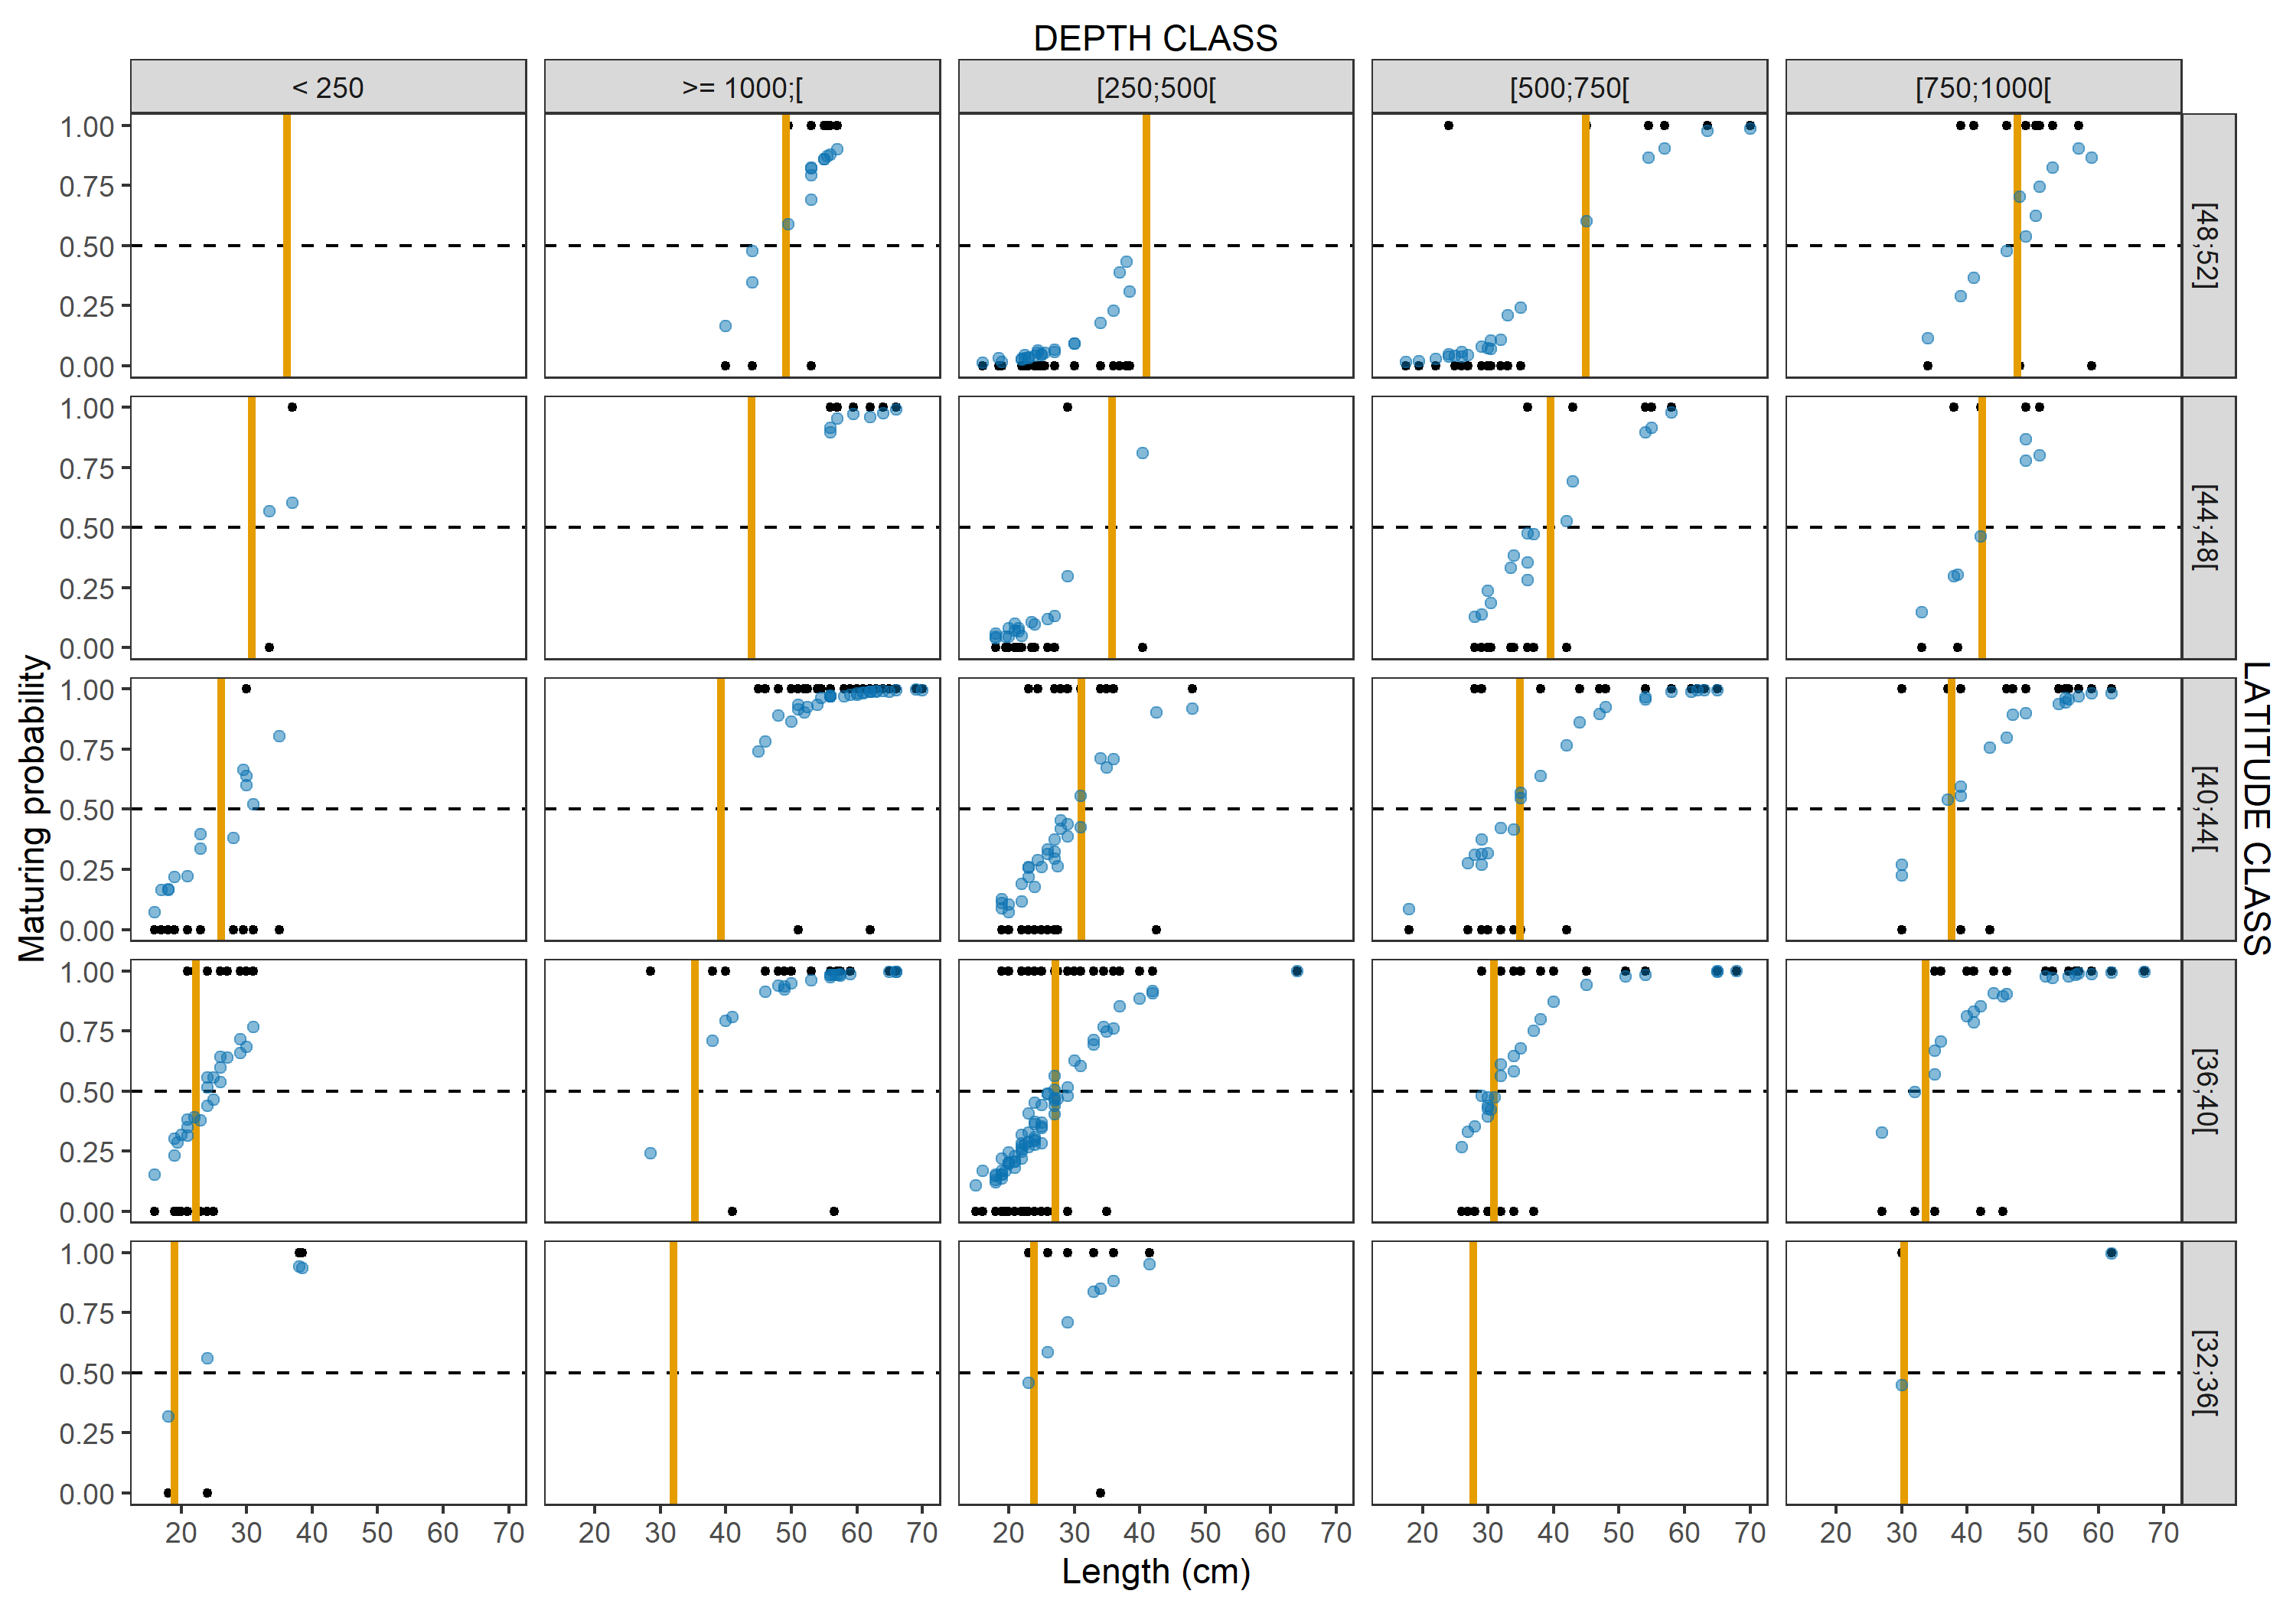
\includegraphics[width=1\textwidth,height=1\textheight]{/Users/jzahner/Desktop/Projects/shortspine_thornyhead_2023/doc/FinalFigs/Data/head2023_maturity_latdepth_glm_fit.png}
\caption{Fit of the maturity curves per size and depth classes. Classes are designed for visual check of the model predictions only since the model assumes continuous and not categorical response to these variables.\label{fig:mat1}}
\end{figure}

\begin{figure}
\centering
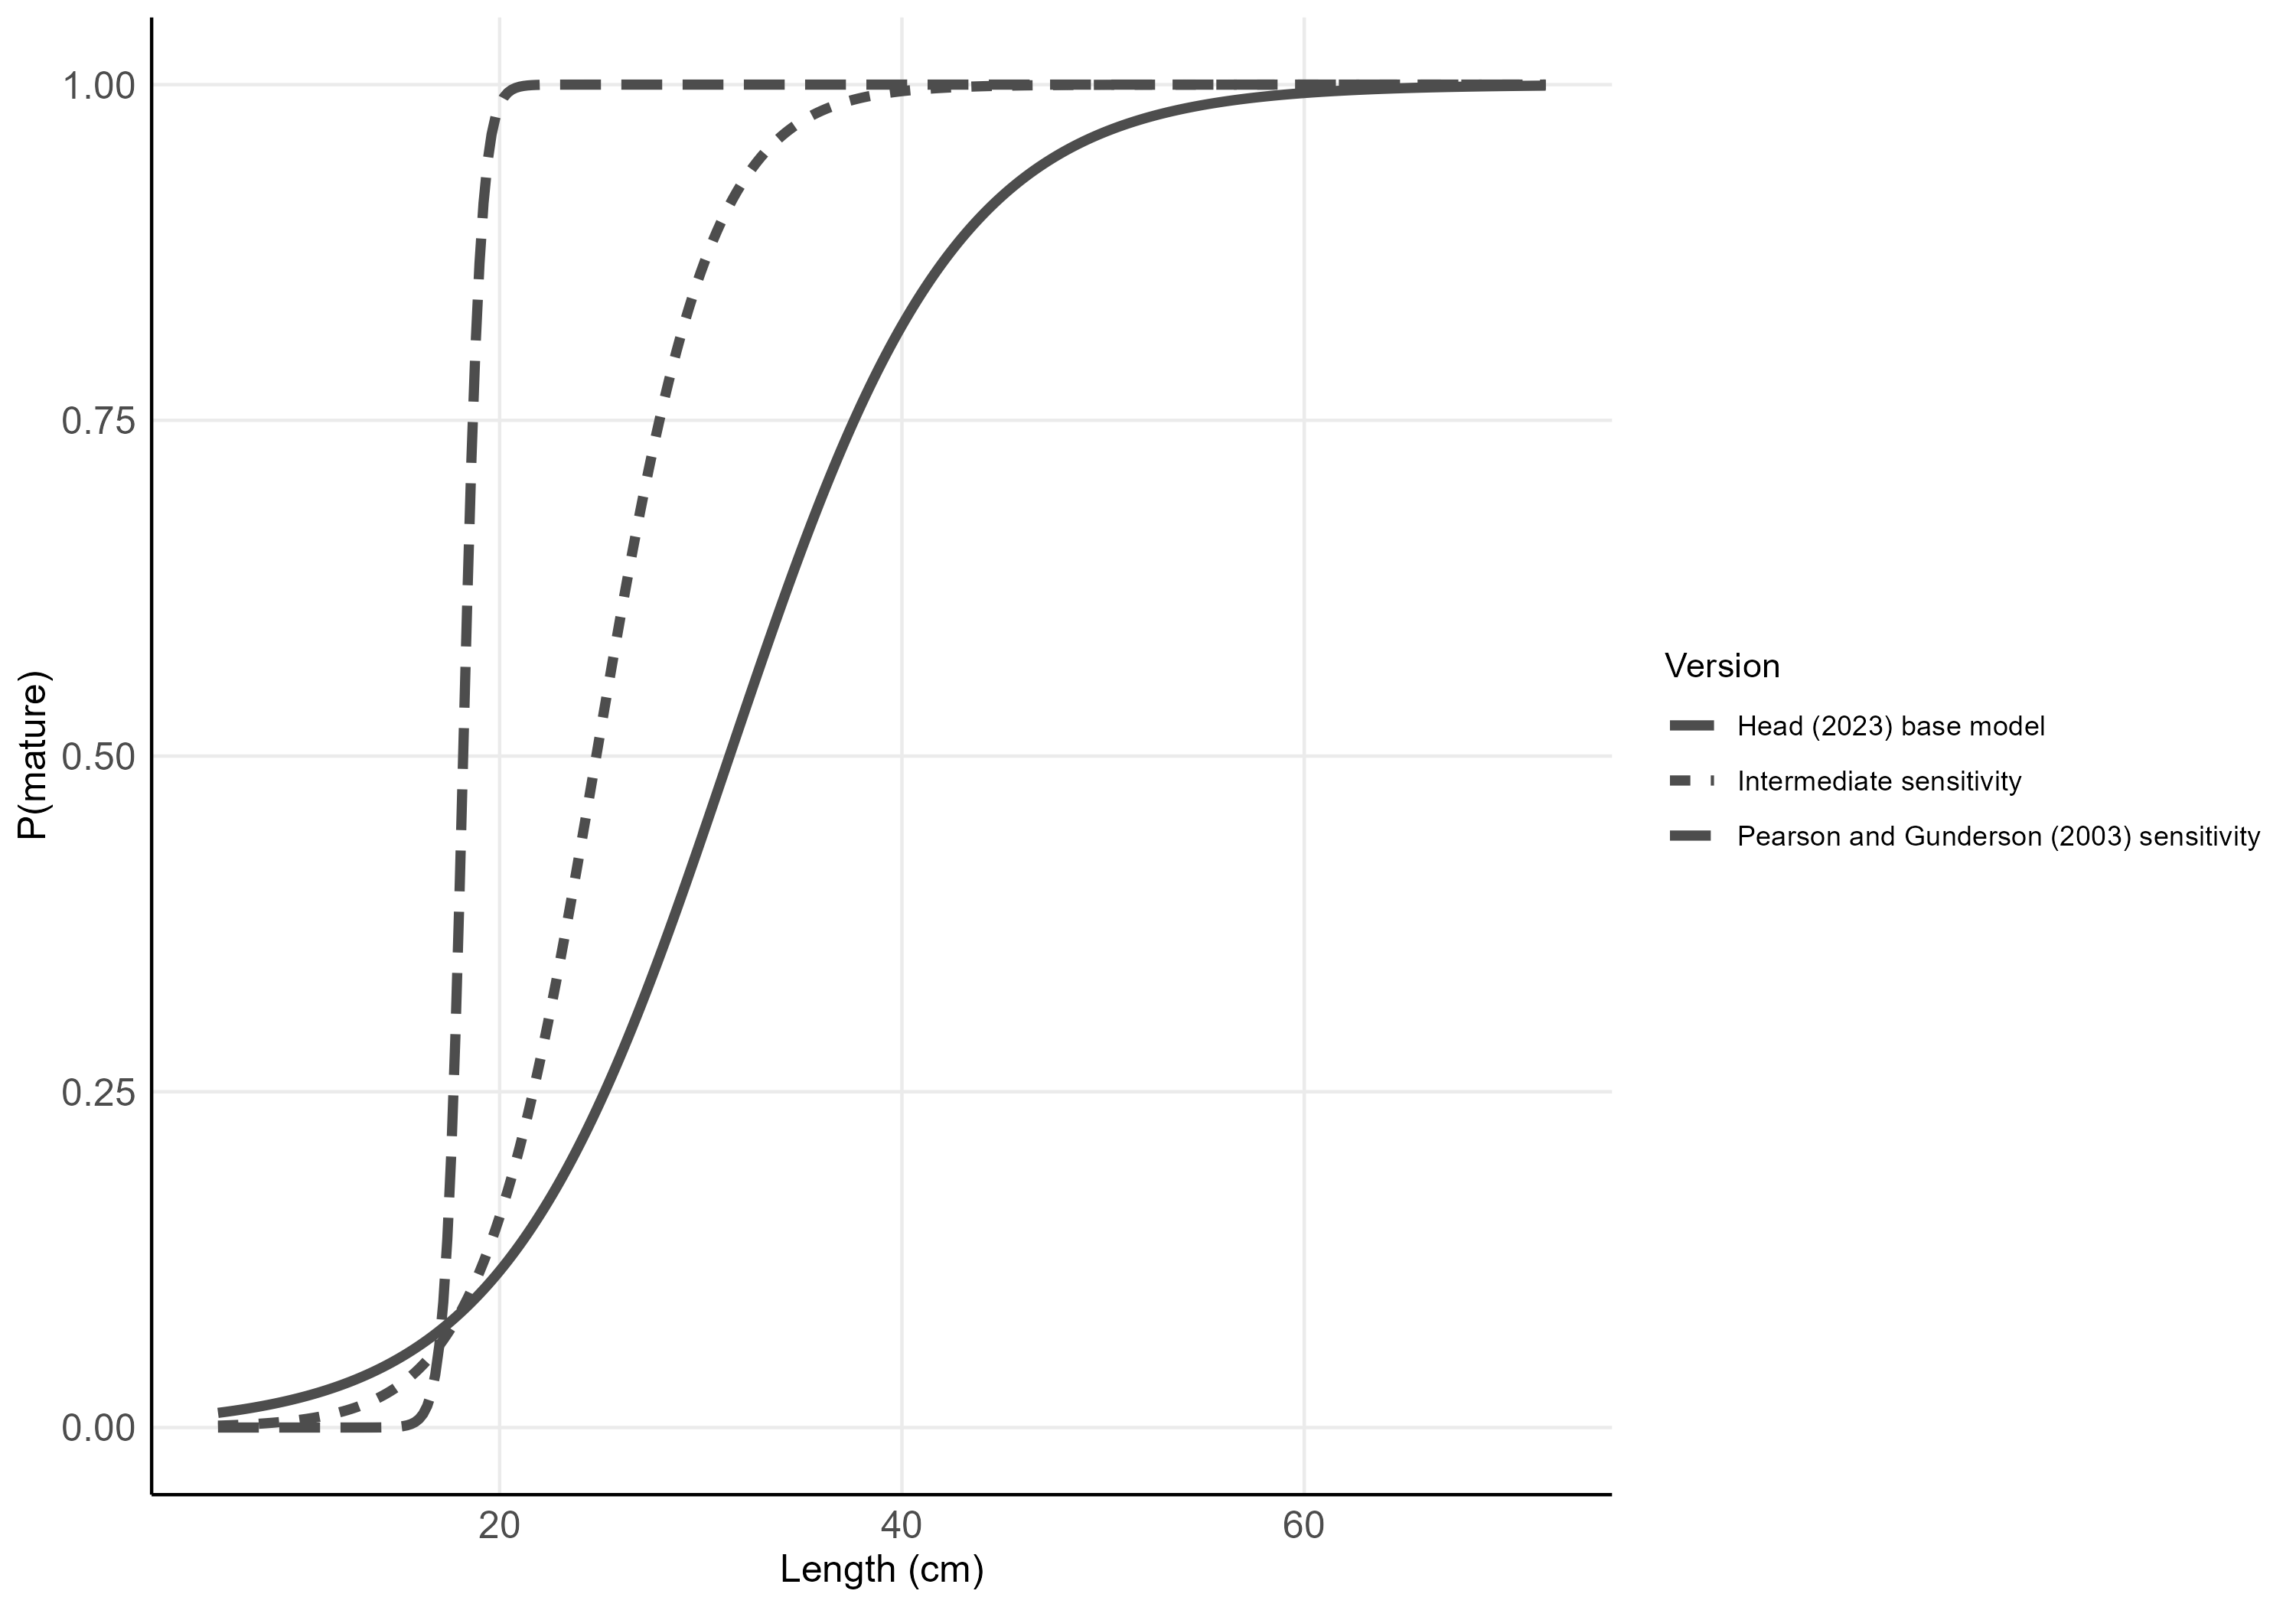
\includegraphics[width=1\textwidth,height=1\textheight]{/Users/jzahner/Desktop/Projects/shortspine_thornyhead_2023/doc/FinalFigs/Data/comparison_alternative_maturity_curves.png}
\caption{Maturity curves considered in the present assessment (Head (2023)) and alternative versions considered in the sensitivity analysis.\label{fig:mat2}}
\end{figure}
\end{document}
